% !TeX encoding = UTF-8
% !TeX spellcheck = es_ES
\documentclass[12pt]{article}
\usepackage{fullpage}
\usepackage[utf8]{inputenc}
\usepackage{pict2e}
\usepackage{amsmath}
\usepackage{enumitem}
\usepackage{eurosym}
\usepackage{mathtools}
\usepackage{amssymb, amsfonts, latexsym, cancel}
\setlength{\parskip}{0.3cm}
\usepackage{graphicx}
\usepackage{fontenc}
\usepackage{setspace}
\usepackage{adjustbox}
\usepackage{float}
\setstretch{1.35}
\usepackage{bold-extra}
\usepackage{subcaption}
\pagestyle{empty}
\graphicspath{ {images/} }
\usepackage{tcolorbox}
\usepackage{xcolor, colortbl}
\usepackage{wrapfig}
\usepackage{empheq}
\usepackage{array}
\usepackage{parskip}
\usepackage{arydshln}
\renewcommand*\contentsname{\color{black}Índice} 
\usepackage{array, multirow, multicol}
\definecolor{lightblue}{HTML}{007AFF}
\usepackage{color}
\usepackage{etoolbox}
\usepackage{listings}
\usepackage{mdframed}
\setlength{\parindent}{0pt}
\usepackage{underscore}
\usepackage{hyperref}
\usepackage{tikz}
\usetikzlibrary{shapes, positioning, patterns}
\usepackage{tikz-qtree}
\usepackage{biblatex}
\usepackage{pdfpages}
\usepackage{pgfplots}
\usepackage{pgfkeys}
\usepackage{mathrsfs}
\addbibresource{biblatex-examples.bib}
\usepackage[a4paper, left=1cm, right=1cm, top=1cm,
bottom=1.5cm]{geometry}
\everymath{\displaystyle}
\usetikzlibrary{decorations, calc, arrows.meta}
\usepackage{titlesec}
\usepackage{pgffor}
\usepackage{subcaption}
\setlength{\fboxrule}{1.5pt}
\renewcommand{\arraystretch}{1.2}

% Configura el formato de las secciones utilizando titlesec
\titleformat{\section}
{\color{red}\normalfont\LARGE\bfseries}
{Tema \thesection:}
{10 pt}
{}

\titleformat{\subsection}
{\normalfont\Large\bfseries\color{red}}{\thesubsection)}{1em}{\color{lightblue}}

\titleformat{\subsubsection}
{\normalfont\large\bfseries\color{red}}{\thesubsubsection)}{1em}{\color{lightblue}}

\newcommand{\bboxed}[1]{\fcolorbox{lightblue}{lightblue!10}{$#1$}}
\newcommand{\rboxed}[1]{\fcolorbox{red}{red!10}{$#1$}}

\newcommand{\bu}[1]{\textcolor{lightblue}{\underline{#1}}}
\newcommand{\lb}[1]{\textcolor{lightblue}{#1}}
\newcommand{\db}[1]{\textcolor{blue}{#1}}
\newcommand{\rc}[1]{\textcolor{red}{#1}}

\newcommand{\dx}{\:\mathrm{d}x}
\newcommand{\dt}{\:\mathrm{d}t}
\newcommand{\dy}{\:\mathrm{d}y}
\newcommand{\dz}{\:\mathrm{d}z}
\newcommand{\dth}{\:\mathrm{d}\theta}
\newcommand{\dr}{\:\mathrm{d}\rho}
\newcommand{\du}{\:\mathrm{d}u}
\newcommand{\dv}{\:\mathrm{d}v}
\newcommand{\tozero}[1]{\cancelto{0}{#1}~~~}
\newcommand{\lbb}[2]{\textcolor{lightblue}{\underbracket[1pt]{\textcolor{black}{#1}}_{#2}}}
\newcommand{\dbb}[2]{\textcolor{blue}{\underbracket[1pt]{\textcolor{black}{#1}}_{#2}}}
\DeclareMathOperator{\N}{\mathbb{N}}
\DeclareMathOperator{\Z}{\mathbb{Z}}
\DeclareMathOperator{\R}{\mathbb{R}}
\DeclareMathOperator{\Q}{\mathbb{Q}}
\DeclareMathOperator{\K}{\mathbb{K}}

\renewcommand{\CancelColor}{\color{lightblue}}

\begin{document}
\begin{enumerate}[label=\color{red}\textbf{\arabic*}),leftmargin=*, start=27]
\item \lb{Calcular los siguientes límites en el caso en el que existan}

$\db{\lim_{n\to\infty}\underset{\color{black}a_n=n}{\sqrt[n]{n}}=(\infty^0)}=\left\{\begin{array}{l}
      \text{Aplicamos el corolario del}\\
      \text{criterio de Stolz}\\
      \lim_{n\to\infty}\sqrt[n]{a_n}=\lim_{n\to\infty}\dfrac{a_{n+1}}{a_n}
\end{array}\right\}=\lim_{n\to\infty}\dfrac{a_{n+1}}{a_{n}}=\lim_{n\to\infty}\dfrac{n+1}{n}=\lim_{n\to\infty}\left(1+\tozero{\dfrac{1}{n}}~\right)=\bboxed{1}$
\item \lb{Sea $(x_n)_n$ una sucesión definida por $x_1=1$ y $x_{n+1=\sqrt{1+x_n}}$ para cada $n\ge1$. Demostrar que la sucesión $(x_n)_n$ es convergente demostrando que es monótona creciente y acotada superiormente. Hallar $\lim_{n\to\infty}x_n$.}

$\begin{cases}
      x_1=\\
      x_{n+1}=\sqrt{1+x_n}
\end{cases}$
\begin{enumerate}[label=\color{lightblue}\arabic*)]
      \item Tomaremos 3 o 4 datos de la sucesión y observamos la tendencia que tiene: \[ \begin{array}{l}
            x_1=1\\
            x_2=\sqrt{1+x_1}=\sqrt{2}\\
            x_3=\sqrt{1+x_2}=\sqrt{1+\sqrt{2}}\\
            x_4=\sqrt{1+x_3}=\sqrt{1+\sqrt{1+\sqrt{2}}}
      \end{array} \] Como podemos observar la tendencia de la sucesión es a ser creciente. Por lo tanto, vamos a demostrar por el principio de inducción que la sucesión es creciente $\forall\:n\in\N$.
      \item Demostración de que $x_n$ es creciente:
      \begin{enumerate}[label=\color{lightblue}\roman*)]
            \item[] $A=\{n\in\N|x_n\le x_{n+1}\}$
            \item ¿$1\in A$?$\longrightarrow x_1\le x_2$ \[ \begin{array}{l}
                  x_1=1\\
                  x_2=\sqrt{2}
            \end{array}\longrightarrow1\le\sqrt{2}\longrightarrow1\in A \]
            \item Supuesto cierto que $n\in A,\:x_n\le x_{n+1}$. Veamos si esto implica que $n+1\in A$, ¿$x_{n+1}\le x_{n+2}$?
            
            Como es cierto que $x_n\le x_{n+1}\longrightarrow 1+x_n\le 1+x_{n+1}\longrightarrow\sqrt{1+x_n}\le\sqrt{1+xn+1}\longrightarrow x_{n+1}\le x_{n+2}\longrightarrow(n+1)\in A$
      \end{enumerate}
            Por lo tanto podemos asegurar que $A=\N\longrightarrow\bboxed{x_n\text{ es creciente }\forall n\in\N.}$
      \item Si estuviese acotada superiormente entonces sería convergente y ocurriría que $\lim_{n\to\infty}x_n=L=\lim_{n\to\infty}x_{n+1}$.
      
      Esto quiere decir que $x_{n+1}=\sqrt{1+x_n}\longrightarrow L=\sqrt{1+L}\longrightarrow L^2=1+L\longrightarrow L^2-L-1=0$ \[ L=\dfrac{1\pm\sqrt{1+4}}{2}=\begin{cases}
            \bboxed{L=\dfrac{1+\sqrt{5}}{2}}<2\\
            L=\dfrac{1-\sqrt{5}}{2}<0\text{ (Como $x_1=1$ y $x_n$ es creciente, es imposible este)}
      \end{cases} \]
      \item Como $x_n$ es creciente y $x_1=1$ si decimos que en caso de ser convergente $L=\dfrac{1+\sqrt{5}}{2}<2$ podemos decir que $x_n$ debería estar acotada superiormente por 2.

Vamos a demostrar por inducción que $x_n$ está acotada superiormente por 2.
\begin{enumerate}[label=\color{lightblue}\roman*)]
      \item[] $A=\{n\in\N|x_n\le 2\}$
      \item ¿$1\in A$? \[x_1=1\le2\longrightarrow 1\in A\]
      \item Supongamos que $n\in A,\:x_n\le2$. Veamos si esto implica que $(n+1)\in A$, es decir, ¿$x_{n+1}\le2$?
      
      Partimos: $x_n\le2\longrightarrow1+x_n\le3\longrightarrow\sqrt{1+x_n}\le\sqrt{3}<2\longrightarrow x_{n+1}<2\longrightarrow (n+1)\in A$
      
      Por lo tanto $A=\N\longrightarrow\bboxed{\text{$x_n$ está acotada superiormente por 2}}$
\end{enumerate}
Como $x_n$ es creciente y acotada superiormente $\longrightarrow x_n$ es convergente $\longrightarrow\bboxed{L=\dfrac{1+\sqrt{5}}{2}}$
\end{enumerate}
\item \lb{Sea $(x_n)_n$ una sucesión definida por $x_1=1$ y $x_{n+1=\sqrt{3x_n}}$ para cada $n\ge1$. Demostrar que la sucesión $(x_n)_n$ es convergente demostrando que es monótona creciente y acotada superiormente. Hallar $\lim_{n\to\infty}x_n$.}
\begin{enumerate}[label=\color{lightblue}\arabic*)]
      \item Tomaremos 3 o 4 valores para observar el funcionamiento de la sucesión: \[ \begin{array}{l}
            x_1=1\\
            x_2=\sqrt{3x_1}=\sqrt{3}\\
            x_3=\sqrt{3x_2}=\sqrt{3\sqrt{3}}
            x_4=\sqrt{3x_3}=\sqrt{3\sqrt{3\sqrt{3}}}
      \end{array} \] Aparentemente la sucesión es creciente, veámoslo aplicado el principio de adicción.
      \item Sea $A=\{n\in\N|x_n\le x_{n+1}\}$
      \begin{enumerate}[label=\color{lightblue}\roman*)]
            \item Veamos si $1\le A$, ¿$x_1\le x_2$? \[ \begin{array}{l}
                  x_1=1\\
                  x_2=\sqrt{3}
            \end{array}\longrightarrow x_1\le x_2\longrightarrow1\in A \]
            \item Supuesto cierto que $n\in A,\:x_n\le x_{n+1}$. Veamos si $(n+1)\in A$, ¿$x_{n+1}\le x_{n+2}$? 
            
            Partimos de lo que hemos supuesto cierto: $$x_n\le x_{n+1}\longrightarrow 3x_n\le3x_{n+1}\longrightarrow \sqrt{3x_n}\le\sqrt{3x_{n+1}}\longrightarrow x_{n+1}\le x_{n+2}\longrightarrow(n+1)\in A$$

      \end{enumerate}  
      Por lo tanto $A=\N\longrightarrow\bboxed{\text{$x_n$ es creciente}}$
      \item Para encontrar la posible cota superior, vamos a suponer que es convergente: \[ \begin{array}{l}
      \lim_{n\to\infty}x_n=L=\lim_{n\to\infty}x_{n+1}\longrightarrow x_{n+1}=\sqrt{3x_n}\xrightarrow[n\to+\infty]{}L)\sqrt{3L} \\
      L^2=3L\longrightarrow L^2-3L=0\longrightarrow L(L-3)=0\begin{cases}
            \xcancel{L=0} \text{(Como $x_1=1$ y es creciente)}\\
            \bboxed{L=3}
      \end{cases}
      \end{array}\]
      \item Vamos a comprobar que $x_n$ está acotada superiormente por 3.
      
      \begin{enumerate}[label=\color{lightblue}\roman*)]
      \item[] Sea $A=\{n\in\N|x_n\le3\}$
      \item ¿$i\in A$? \[ x_1=1\le3\longrightarrow x_1\le3\longrightarrow1\le A \]
      \item Supuesto cierto que $n\in A,\:x_n\le3$. Veamos que también se cumple que $(n+1)\in A$, ¿$x_{n+1}\le3$?
      
      Partimos de que: $x_n\le3\longrightarrow3x_n\le9\longrightarrow\sqrt{3x_n}\le\sqrt{9}=3\longrightarrow x_{n+1}\le3\longrightarrow(n+1)\in A$
      
      Por lo tanto $A=\N\longrightarrow\bboxed{\text{$x_n$ está acotada superiormente por 3}}$
      \end{enumerate}
      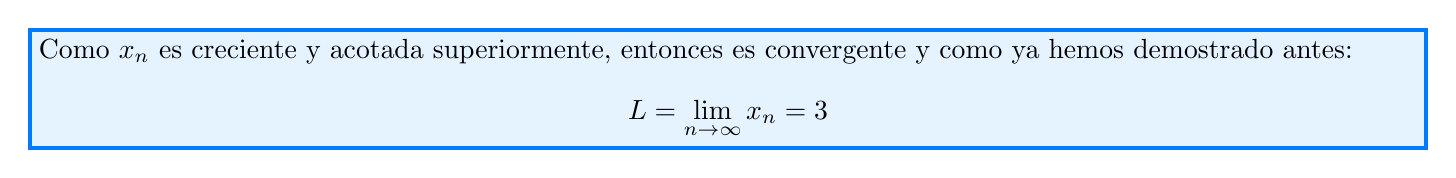
\begin{tikzpicture}
            \node[draw=lightblue,fill=lightblue!10,rectangle,line width=1.5pt,text width=17.5cm] {Como $x_n$ es creciente y acotada superiormente, entonces es convergente y como ya hemos demostrado antes: \[ L=\lim_{n\to\infty}x_n=3 \]};
      \end{tikzpicture}
\end{enumerate}
\item \lb{Hallar la suma de las series}

$\db{\sum_{n=1}^{\infty}\dfrac{1}{2n(n+1)}}$

Lo primero que debemos hacer antes de ponernos a sumar una serie, es comprobar si es convergente o divergente, ya que si fuese divergente directamente diríamos que su suma es $+\infty$.

Como tenemos un cociente de polinomios, para estudiar su convergencia utilizaremos el criterio de las series asintóticamente proporcionales, comparando siempre con la serie armónica $\sum_{n=1}^{+\infty}\dfrac{1}{n^p}$ donde $p$ deberá ser la diferencia entre el grado de polinomio del denominador y el grado del polinomio del numerador.

\begin{minipage}[h]{\linewidth}

\begin{wrapfigure}{r}{0.3\linewidth}
            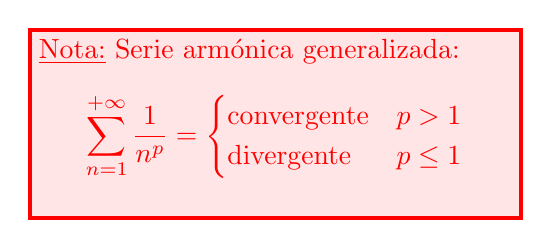
\begin{tikzpicture}
      \node[red,draw=red,fill=red!10,line width=1.5pt,text width=6cm] {\underline{Nota:} Serie armónica generalizada: \[ \sum_{n=1}^{+\infty}\dfrac{1}{n^p}=\begin{cases}
                  \text{convergente} &p>1\\
                  \text{divergente} & p\le1
            \end{cases} \]};
\end{tikzpicture}
\end{wrapfigure}

Para estudiar la convergencia de esta serie, aplicaremos el criterio de las series asintóticamente proporcionales: \[ \lim_{n\to\infty}\dfrac{\frac{1}{2n(n+1)}}{\frac{1}{n^2}}=\lim_{n\to\infty}\dfrac{n^{\cancel{2}}}{2\cancel{n}(n+1)}=\lim_{n\to\infty}\dfrac{n}{2n+2}=\left(\dfrac{\infty}{\infty}\right)=\lim_{n\to\infty}\dfrac{\frac{n}{n}}{\frac{2n}{n}+\tozero{\frac{2}{n}}} \]
Por lo tanto, ambas series tienen el mismo carácter.
\end{minipage}


\begin{minipage}{\linewidth}
\begin{wrapfigure}{r}{0.3\linewidth}
      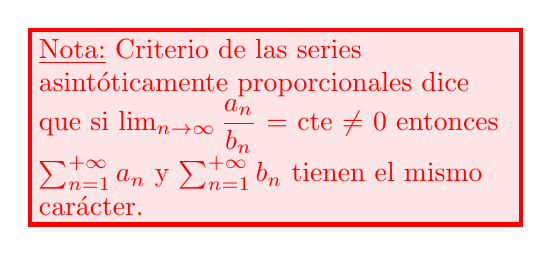
\begin{tikzpicture}
      \node[red,draw=red,fill=red!10,line width=1.5pt,text width=6cm] {\underline{Nota:} Criterio de las series asintóticamente proporcionales dice que si $\lim_{n\to\infty}\dfrac{a_n}{b_n}=\mathrm{cte}\neq0$ entonces $\sum_{n=1}^{+\infty}a_n$ y $\sum_{n=1}^{+\infty}b_n$ tienen el mismo carácter.};
\end{tikzpicture}
\end{wrapfigure}

Como $\sum_{n=1}^{+\infty}\dfrac{1}{n^2}$ es la serie armónica generalizada con $p=2>1$ es convergente $\longrightarrow\sum_{n=1}^{+\infty}\dfrac{1}{2n(n+1)}$ también es convergente.
\end{minipage}

\vspace{2.5cm}

Una vez comprobado que es convergente lo que haremos será sumarla. Al ser un cociente de polinomios será una serie telescópica. \[ \begin{array}{l}
      \sum_{n=1}^{+\infty}\dfrac{1}{2n(n+1)}=\dfrac{1}{2}\cdot\sum_{n=1}^{+\infty}\underset{\color{lightblue}\begin{subarray}{l}
                  \text{Separación por}\\
                  \text{fracciones simples}
      \end{subarray}}{\bboxed{\dfrac{1}{n(n+1)}}}=\lb{(\ast)}\\
\dfrac{1}{n(n+1)}=\dfrac{A}{n}+\dfrac{B}{n+1}=\dfrac{A(n+1)+Bn}{n(n+1)}\longrightarrow1=A(n+1)+Bn\\
\begin{array}{l}
      \text{Si }n=0\longrightarrow A=1\\
      \text{Si }n=-1\longrightarrow B=-1
\end{array}\longrightarrow\dfrac{1}{n(n+1)}=\dfrac{1}{n}-\dfrac{1}{n+1}\\
\lb{(\ast)=}\dfrac{1}{2}\cdot\sum_{n=1}^{\infty}\left[\dfrac{1}{n}-\dfrac{1}{n+1}\right]=\dfrac{1}{2}\lim_{n\to\infty}\underset{\lb{S_n}}{\bboxed{\sum_{j=1}^{n}\left[\dfrac{1}{j}-\dfrac{1}{j+1}\right]}}=\dfrac{1}{2}\lim_{n\to\infty}\left(1-\tozero{\dfrac{1}{n+1}}\right)=\bboxed{\dfrac{1}{2}}\\
\lb{S_n=}\sum_{j=1}^{n}\left[\lbb{\dfrac{1}{j}}{~}-\dbb{\dfrac{1}{j+1}}{~}\right]=\left\{\begin{array}{r|c|l}
      \bboxed{1} & \bcancel{+\dfrac{1}{2}+\dfrac{1}{3}+\dfrac{1}{4}+\cdots+\dfrac{1}{n}} & \\
       & \bcancel{-\dfrac{1}{2}-\dfrac{1}{3}-\dfrac{1}{4}-\cdots-\dfrac{1}{n}} & \bboxed{-\dfrac{1}{n+1}}
\end{array}\right\}=1-\dfrac{1}{n+1}
\end{array} \]
\item \lb{Hallar la suma de las series:}

$\db{\sum_{n=1}^{\infty}\dfrac{1}{n(n+3)}}$

Antes de ponernos a sumarla, lo primero que debemos hacer es comprobar que sea convergente. En este caso, como es un cociente de polinomios compararemos con $\sum_{n=1}^{+\infty}\dfrac{1}{n^p}$ aplicando el criterio de las series asintóticamente proporcionales. \[ \lim_{n\to\infty}\dfrac{\frac{1}{n(n+3)}}{\frac{1}{n^2}}=\lim_{n\to\infty}\dfrac{n^{\cancel{2}}}{\cancel{n}(n+3)}=\lim_{n\to\infty}\dfrac{n}{n+3}=\left(\dfrac{\infty}{\infty}\right)=\lim_{n\to\infty}\dfrac{\frac{n}{n}}{\frac{n}{n}+\tozero{\frac{3}{n}}}=1\neq0 \]Por lo tanto, ambas series tienen el mismo carácter.

Como $\sum_{n=1}^{\infty}\dfrac{1}{n^2}$ es la serie armónica generalizada con $p=2>1\longrightarrow $ Es convergente $\longrightarrow\sum_{n=1}^{\infty}\dfrac{1}{n(n+3)}$ \lb{será convergente}

Para sumarla, como es un cociente de polinomios debemos factorizar el denominador y separar por fracciones simples: \[ \dfrac{1}{n(n+3)}=\dfrac{A}{n}+\dfrac{B}{n+3}=\dfrac{A(n+3)+Bn}{n(n+3)}\longrightarrow1=A(n+3) +Bn\begin{cases}
      \text{Si }n=0\longrightarrow A=\dfrac{1}{3}\\
      \text{Si }n=-3\longrightarrow B=-\dfrac{1}{3}
\end{cases}\]
Por lo tanto, tenemos que: \[ \sum_{n=1}^{\infty}\dfrac{1}{n(n+3)}=\sum_{n=1}^{\infty}\left[\dfrac{\frac{1}{3}}{n}-\dfrac{\frac{1}{3}}{n+3}\right] =\dfrac{1}{3}\sum_{n=1}^{\infty}\left[\dfrac{1}{n}-\dfrac{1}{n+3}\right]=\dfrac{1}{3}\lim_{n\to\infty}\underset{\lb{S_n}}{\bboxed{\sum_{j=1}^{n}\left[\dfrac{1}{j}-\dfrac{1}{j+3}\right]}}=\lb{(\ast)}\]

$\begin{array}{l}
      \begin{aligned}
      \lb{S_n=}\sum_{j=1}^{n}\left[\lbb{\dfrac{1}{j}}{~}-\dbb{\dfrac{1}{j+3}}{~}\right]&=\left\{\begin{array}{r|c|l}
      1+\dfrac{1}{2}+\dfrac{1}{3} & \bcancel{+\dfrac{1}{4}+\dfrac{1}{5}+\cdots+\dfrac{1}{n}} & \\
      & \bcancel{-\dfrac{1}{4}-\dfrac{1}{5}-\cdots-\dfrac{1}{n}} &-\dfrac{1}{n+1}-\dfrac{1}{n+2}-\dfrac{1}{n+3}
\end{array}\right\}\\
&=1+\dfrac{1}{2}+\dfrac{1}{3}-\dfrac{1}{n+1}-\dfrac{1}{n+2}-\dfrac{1}{n+3}
\end{aligned}\\
\lb{(\ast)=}\dfrac{1}{3}\lim_{n\to\infty}\left[1+\dfrac{1}{2}+\dfrac{1}{3}-\tozero{\dfrac{1}{n+1}}-\tozero{\dfrac{1}{n+2}}-\tozero{\dfrac{1}{n+3}}\right]=\dfrac{1}{3}\left[\dfrac{11}{6}\right]=\bboxed{\dfrac{11}{18}}
\end{array}$
\item \lb{Estudiar la convergencia de las series:}

$\db{\sum_{n=1}^{\infty}\dfrac{1}{\sqrt{n^3+2n+2}}}$

Para estudiar la convergencia de esta serie, utilizaremos el criterio de las series asintóticamente proporcionales comparando con $ \sum_{n=1}^{\infty}\dfrac{1}{n^{\frac{3}{2}}}$ \[ \lim_{n\to\infty}\dfrac{\frac{1}{\sqrt{n^3
2n
2}}}{\frac{1}{\sqrt{n^3}}}=\lim_{n\to\infty}\dfrac{\sqrt{n^3}}{\sqrt{n^3+2n+2}}=\lim_{n\to\infty}\sqrt{\dfrac{n^3}{n^3+2n+2}}=\left(\dfrac{\infty}{\infty}\right)=\lim_{n\to\infty}\sqrt{\dfrac{\frac{n^3}{n^3}}{\frac{n^3}{n^3}+\tozero{\frac{2n}{n^3}}+\tozero{\frac{2}{n^3}}}}=1\neq0\]Ambas series tienen el mismo carácter

Como $\sum_{n=1}^{\infty}\dfrac{1}{n^{\frac{3}{2}}}$ es la serie armónica generalizada con $p=\dfrac{3}{2}>1$ entonces es convergente\\
 $\longrightarrow\bboxed{\sum_{n=1}^{\infty}\dfrac{1}{\sqrt{n^3+2n+2}}\text{ es convergente}}$
 \item \lb{Hallar la suma de las series:}
 
 $\db{\sum_{n=3}^{\infty}\dfrac{1}{n^2-n}}$
 
 Lo primero que vamos a hacer es comprobar si la serie es convergente o no. Para ello, como es cociente de polinomios utilizaremos el criterio de las series asintóticamente proporcionales, en concreto compararemos $ \sum_{n=1}^{\infty}\dfrac{1}{n^2}$. \[ \lim_{n\to\infty}\dfrac{\frac{1}{n^2-n}}{\frac{1}{n^2}}=\lim_{n\to\infty}\dfrac{n^2}{n^2-n}=\left(\dfrac{\infty}{\infty}\right)=\lim_{n\to\infty}\dfrac{\frac{n^2}{n^2}}{\frac{n^2}{n^2}-\tozero{\frac{n}{n^2}}}=1\neq0\quad\text{Ambas series tienen el mismo carácter} \] Como $\sum_{n=1}^{\infty}\dfrac{1}{n^2}$ es la serie armónica generalizada con $p=2>1\longrightarrow$ es convergente. Por lo tanto: $\sum_{n=3}^{\infty}\dfrac{1}{n^2-n}$ es convergente. 
 \[ \begin{array}{l}
       \sum_{n=3}^{\infty}\dfrac{1}{n^2-n}=\sum_{n=3}^{\infty}\dfrac{1}{n(n-1)}=\lb{(\ast)}\\
       \dfrac{1}{n(n-1)}=\dfrac{A}{n}+\dfrac{B}{n-1}=\dfrac{A(n-1)+Bn}{n(n-1)}\longrightarrow1=A(n-1)+Bn\begin{cases}
             \text{Si }n=0\longrightarrow A=-1\\
             \text{Si }n=1\longrightarrow B=1
       \end{cases}\\
       \lb{(\ast)=}\sum_{n=3}^{\infty}\left[-\dfrac{1}{n}+\dfrac{1}{n-1}\right]=\lim_{n\to\infty}\underset{\lb{S_n}}{\bboxed{\sum_{j=3}^{n}\left[-\dfrac{1}{j}+\dfrac{1}{j-1}\right]}}=\lim_{n\to\infty}\left(\dfrac{1}{2}-\tozero{\dfrac{1}{n}}~\right)=\bboxed{\dfrac{1}{2}}\\
       \lb{S_n=}\left\{\begin{array}{r|c|l}
             \dfrac{1}{2} & \bcancel{+\dfrac{1}{3}+\dfrac{1}{4}\cdots+\dfrac{1}{n-1}} & \\
                   & \bcancel{-\dfrac{1}{3}-\dfrac{1}{4}-\cdots-\dfrac{1}{n-1}} & -\dfrac{1}{n}
       \end{array}\right\}=\dfrac{1}{2}-\dfrac{1}{n}
 \end{array} \]
 \item \lb{Hallar la suma de las series:}
 
 $\db{\sum_{n=0}^{\infty}\dfrac{1}{(n+1)(n+3)}}$
 
 Lo primero que vamos a hacer es comprobar si la serie es convergente o no. Para ello, lo que haremos será aplicar el criterio de las series asintóticamente proporcionales, comparándolo con $\sum_{n=1}^{\infty}\dfrac{1}{n^2}$. \[ \lim_{n\to\infty}\dfrac{\frac{1}{(n+1)(n+3)}}{\frac{1}{n^2}}=\lim_{n\to\infty}\dfrac{n^2}{(n+1)(n+3)}=\left(\dfrac{\infty}{\infty}\right)=\lim_{n\to\infty}\dfrac{n^2}{n^2+4n+3}=\lim_{n\to\infty}\dfrac{\frac{n^2}{n^2}}{\frac{n^2}{n^2}+\tozero{\frac{4n}{n^2}}+\tozero{\frac{3}{n^2}}}=1\neq0 \]
 Por lo tanto podemos asegurar que ambas series tienen el mismo carácter.
 
 Como $\sum_{n=1}^{\infty}\dfrac{1}{n^2}$ es la serie armónica generalizada con $p=2>1$ entonces es convergente, por lo tanto $\sum_{n=0}^{\infty}\dfrac{1}{(n+1)(n+3)}$ es convergente.
 
 Para sumarla. (Serie telescópica)
 \[ \begin{array}{l}
       \sum_{n=0}^{\infty}\dfrac{1}{(n+1)(n+3)}=\lb{(\ast)}\\
       \dfrac{1}{(n+1)(n+3)}=\dfrac{A}{n+1}+\dfrac{B}{n+3}=\dfrac{A(n+3)+B(n+1)}{(n+1)(n+3)}\longrightarrow 1=A(n+3)+B(n+1)\\
       \begin{cases}
             \text{Si }n=-1\longrightarrow1=2A\longrightarrow A=\dfrac{1}{2}\\
             \text{Si }n=-3\longrightarrow1=-2B\longrightarrow B=-\dfrac{1}{2}
       \end{cases}\\
       \lb{(\ast)=}\sum_{n=0}^{\infty}\left(\dfrac{\frac{1}{2}}{n+1}-\dfrac{\frac{1}{2}}{n+3}\right)=\dfrac{1}{2}\lim_{n\to\infty}\underset{\lb{S_n}}{\bboxed{\sum_{j=0}^{n}\left(\dfrac{1}{j+1}-\dfrac{1}{j+3}\right)}}=\dfrac{1}{2}\lim_{n\to\infty}\left(1+\dfrac{1}{2}-\tozero{\dfrac{1}{n+2}}-\tozero{\dfrac{1}{n+3}}\right)=\bboxed{\dfrac{3}{4}}\\
       \lb{S_n=}\left\{\begin{array}{r|c|l}
             1+\dfrac{1}{2} & \bcancel{+\dfrac{1}{3}+\dfrac{1}{4}+\cdots+\dfrac{1}{n+1}} & \\
             & \bcancel{-\dfrac{1}{3}-\dfrac{1}{4}-\cdots-\dfrac{1}{n+1}} & -\dfrac{1}{n+2} -\dfrac{1}{n+3}
       \end{array}\right\}=1+\dfrac{1}{2}-\dfrac{1}{n+2}-\dfrac{1}{n+3}
 \end{array} \]
 
 \pagebreak
 \item \lb{Hallar la suma de las series:}
 
 \begin{minipage}{\linewidth}
       \begin{wrapfigure}[7]{r}{0.55\textwidth}
             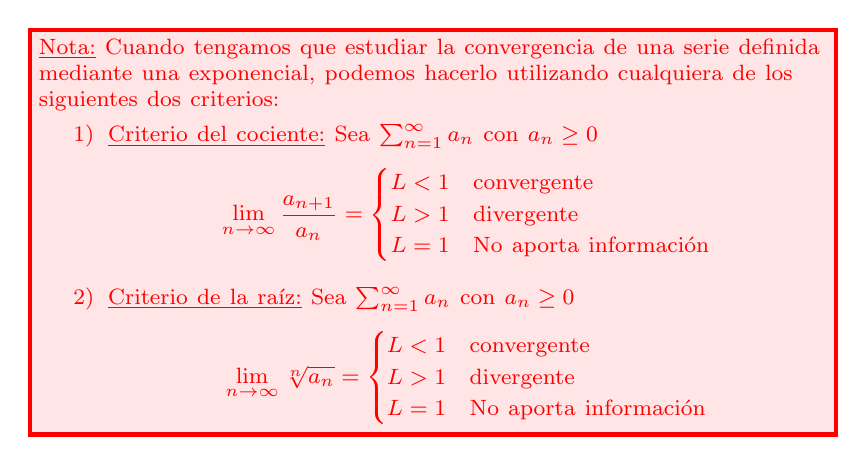
\begin{tikzpicture}[baseline=(current bounding box.center)]
                   \node[red,draw=red,fill=red!10,line width=1.5pt,text width=10cm] {\footnotesize\underline{Nota:} Cuando tengamos que estudiar la convergencia de una serie definida mediante una exponencial, podemos hacerlo utilizando cualquiera de los siguientes dos criterios:\begin{enumerate}[label=\arabic*)]
                               \item \underline{Criterio del cociente:} Sea $\sum_{n=1}^{\infty}a_n$ con $a_n\ge0$ \[ \lim_{n\to\infty}\dfrac{a_{n+1}}{a_n}=\begin{cases}
                                     L<1 & \text{convergente}\\
                                     L>1 & \text{divergente}\\
                                     L=1 & \text{No aporta información}
                               \end{cases} \]
                               \item \underline{Criterio de la raíz:} Sea $\sum_{n=1}^{\infty}a_n$ con $a_n\ge0$ \[ \lim_{n\to\infty}\sqrt[n]{a_n}=\begin{cases}
                                     L<1 & \text{convergente}\\
                                     L>1 & \text{divergente}\\
                                     L=1 & \text{No aporta información}
                               \end{cases} \]
                   \end{enumerate}};
             \end{tikzpicture}
       \end{wrapfigure}
        $\db{\sum_{n=0}^{+\infty}\dfrac{3}{10^n}=}3\cdot\sum_{n=0}^{+\infty}\dfrac{1}{10^n}$
        
        Para estudiar la convergencia de esta serie, aplicaremos el criterio de la raíz: \begin{center}
              $\lim_{n\to\infty}\sqrt[\cancel{n}]{\left(\dfrac{1}{10}\right)^{\cancel{n}}}=\dfrac{1}{10}<1$. Por lo tanto la serie es \lb{convergente}
        \end{center}
        
              $\sum_{n=0}^{+\infty}\dfrac{3}{10^n}=3\sum_{n=0}^{+\infty}\left(\dfrac{1}{10}\right)^n=\left\{\begin{array}{l}
              b_n=\left(\dfrac{1}{10}\right)^n\\
              r=\dfrac{1}{10}
        \end{array}\right\}=3\cdot\sum_{n=0}^{+\infty}b_n=3\lim_{n\to\infty}\underset{\lb{S_n}}{\bboxed{\sum_{j=0}^{n}b_j}}=\lb{(\ast)}$
        
        \begin{wrapfigure}{r}{0.5\textwidth}
              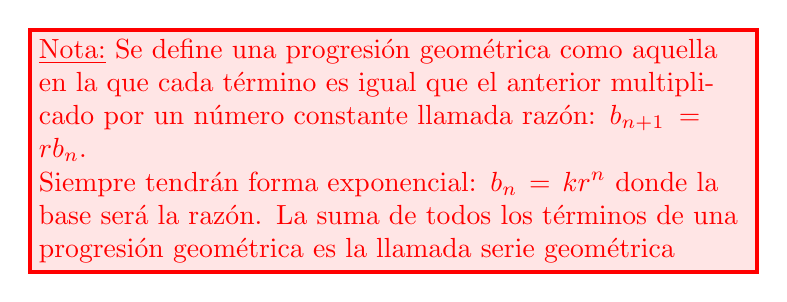
\begin{tikzpicture}
                    \node[red,draw=red,fill=red!10,line width=1.5pt,text width=9cm] {\underline{Nota:} Se define una progresión geométrica como aquella en la que cada término es igual que el anterior multiplicado por un número constante llamada razón: $b_{n+1}=rb_n$.\\
                          Siempre tendrán forma exponencial: $b_{n}=kr^n$ donde la base será la razón. La suma de todos los términos de una progresión geométrica es la llamada serie geométrica};
              \end{tikzpicture}
        \end{wrapfigure}
        $\begin{array}{l|c|l}
              S_n=b_0&+b_1+b_2+b_3+\cdots+b_n & \\
              rS_n= & -b_1+b_2+b_3+\cdots+b_n&+b_{n+1}\\ \hline
              \multicolumn{3}{l}{\text{\underline{resto} }(1-r)S_n=b_0-b_{n+1}\longrightarrow S_n=\frac{b_0-b_{n+1}}{1-r}}
        \end{array}$
        
        $\lb{(\ast)=} 3\lim_{n\to\infty}\dfrac{\left(\frac{1}{10}\right)^0-\tozero{\left(\frac{1}{10}\right)^{n+1}}}{1-\frac{1}{10}}=3\cdot\dfrac{1}{\frac{8}{10}}=\bboxed{\dfrac{10}{3}}$
 \end{minipage}
 \newpage
 \item \lb{Hallar la suma de las series:}
 
 $\db{\sum_{n=3}^{+\infty}\dfrac{1}{2^{n-1}}=}\sum_{n=3}^{+\infty}\dfrac{1}{2^n\cdot 2^{-1}}=\sum_{n=3}^{+\infty}\dfrac{2}{2^n}=2\sum_{n=3}^{+\infty}\dfrac{1}{2^n}$
 \\
 
 Para estudiar la convergencia de esta serie, lo que vamos a hacer es aplicar el criterio de la raíz: \[ \lim_{n\to\infty}\sqrt[\cancel{n}]{\dfrac{1}{2^{\cancel{n}}}}\longrightarrow\text{Convergente} \] Por lo tanto, la serie es convergente y vamos a sumarlo: \[ \begin{array}{l}
       \begin{aligned}
             \sum_{n=3}^{+\infty}\dfrac{1}{2^{n+1}}&=2\cdot\sum_{n=3}^{+\infty}\left(\dfrac{1}{2}\right)^n=\left\{\begin{array}{l}
             b_n=\left(\dfrac{1}{2}\right)^n
       \end{array}\right\}=2\cdot\sum_{n=3}^{+\infty}b_n=2\lim_{n\to\infty}\underset{\lb{S_n}}{\bboxed{\sum_{j=3}^{n}b_j}}=\lb{(\ast)}\\
       &=2\lim_{n\to\infty}\left[\dfrac{\left(\frac{1}{2}\right)^3-\tozero{\left(\frac{1}{2}\right)^{n+1}}}{1-\frac{1}{2}}\right]=2\cdot\dfrac{\frac{1}{8}}{\frac{1}{2}}=\bboxed{\dfrac{1}{2}}
       \end{aligned}\\
       \lb{(\ast)}\qquad\begin{array}{l|c|l}
             S_n=b_3&\bcancel{+b_4+b_5+\cdots+b_n} & \\
             rS_n= & \bcancel{-b_4-b_5-\cdots-b_n} &+b_{n+1}\\ \hline
             \multicolumn{3}{l}{\text{\underline{resto} }(1-r)S_n=b_3-b_{n+1}\longrightarrow S_n=\dfrac{b_3-b_{n+1}}{1-r}}
       \end{array}
 \end{array} \]
 \item \lb{Demostrar la convergencia y hallar la suma de las series:}
 
 $\db{\sum_{n=1}^{\infty}\dfrac{1}{n(n+1)(n+2)}}$
 
 Para demostrar la convergencia lo que vamos a hacer es que al ser un cociente de polinomios, vamos a aplicar el criterio de las series asintóticamente proporcionales, donde compararemos con $\sum_{n=1}^{\infty}\dfrac{1}{n^3}$ \[ \lim_{n\to\infty}\dfrac{\frac{1}{\cancel{n}(n+1)(n+2)}}{\frac{1}{n^{\cancel{3}\lb{2}}}}=\lim_{n\to\infty}\dfrac{n^2}{(n+1)(n+2)}=\lim_{n\to\infty}\dfrac{n^2}{n^2+2n+2}=\left(\dfrac{\infty}{\infty}\right)=\lim_{n\to\infty}\dfrac{\frac{n^2}{n^2}}{\frac{n^2}{n^2}+\tozero{\frac{3n}{n^2}}+\tozero{\frac{2}{n^2}}}=1\neq0 \] Ambas series tienen el mismo carácter.
 Como $\sum_{n=1}^{\infty}\dfrac{1}{n^3}$ es convergente por ser la serie armónica generalizada con $p=3>1$ entonces podemos asegurar que $\sum_{n=1}^{\infty}\dfrac{1}{n(n+1)(n+2)}$ es convergente.
 
 Para sumar esta serie la vamos a trabajar como una serie telescópica y aplicaremos separación por fracciones simples. \[ \dfrac{1}{n(n+1)(n+2)}=\dfrac{A}{n}+\dfrac{B}{n+1}+\dfrac{C}{n+2}=\dfrac{A(n+1)(n+2)+Bn(n+2)+Cn(n+1)}{n(n+1)(n+2)} \]
 $\begin{array}{l}
       1=A(n+1)(n+2)+Bn(n+2)+Cn(n+1)\\
       \text{Si }n=0\longrightarrow1=2A\longrightarrow A=\dfrac{1}{2}\\
       \text{Si }n=-1\longrightarrow1=-B\longrightarrow B=-1\\
       \text{Si }n=-2\longrightarrow1=2C\longrightarrow C=\dfrac{1}{2}
 \end{array} $\qquad
  \begin{minipage}[l]{0.5\textwidth}
        
       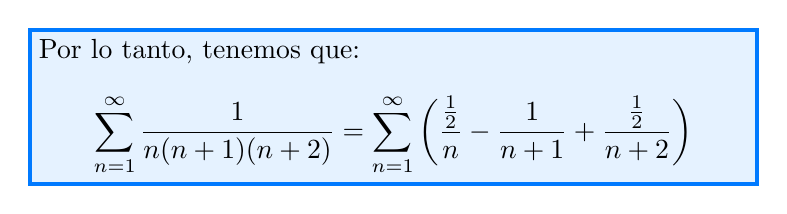
\begin{tikzpicture}[baseline=(current bounding box.center)]
             \node[draw=lightblue,fill=lightblue!10,line width=1.5pt,text width=9cm] {Por lo tanto, tenemos que: \[ \sum_{n=1}^{\infty}\dfrac{1}{n(n+1)(n+2)}=\sum_{n=1}^{\infty}\left(\dfrac{\frac{1}{2}}{n}-\frac{1}{n+1}+\dfrac{\frac{1}{2}}{n+2}\right) \]};
       \end{tikzpicture}
 \end{minipage}
 
\begin{minipage}[l]{0.6\textwidth}
       $\sum_{n=1}^{\infty}\left(\dfrac{\frac{1}{2}}{n}-\frac{1}{n+1}+\dfrac{\frac{1}{2}}{n+2}\right)=\sum_{n=1}^{\infty}\left(\dfrac{\frac{1}{2}}{n}-\dfrac{\frac{1}{2}}{n+1}-\dfrac{\frac{1}{2}}{n+1}+\dfrac{\frac{1}{2}}{n+2}\right)=\dfrac{1}{2}\lbb{\sum_{n=1}^{\infty}\left(\dfrac{1}{n}-\dfrac{1}{n+1}\right)}{S_1}+\dfrac{1}{2}\dbb{\sum_{n=1}^{\infty}\left(-\dfrac{1}{n+1}+\dfrac{1}{n+2}\right)}{S_2}$
\end{minipage}\qquad
\begin{minipage}[l]{0.4\textwidth}
      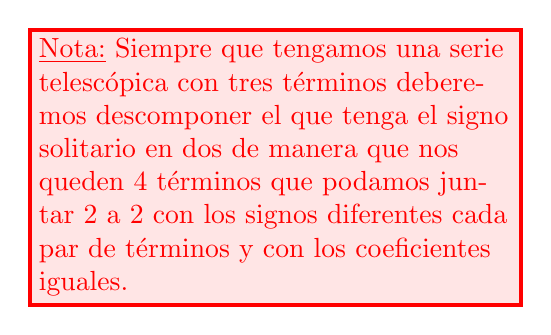
\begin{tikzpicture}[baseline=(current bounding box.center)]
            \node[red,draw=red,fill=red!10,line width=1.5pt,text width=6cm] {\underline{Nota:} Siempre que tengamos una serie telescópica con tres términos deberemos descomponer el que tenga el signo solitario en dos de manera que nos queden 4 términos que podamos juntar 2 a 2 con los signos diferentes cada par de términos y con los coeficientes iguales.};
      \end{tikzpicture}
\end{minipage}

$\begin{array}{l}
      \lb{S_1=}\sum_{n=1}^{\infty}\left(\dfrac{1}{n}-\dfrac{1}{n+1}\right)=\lim_{n\to\infty}\lbb{\sum_{j=1}^{n}\left(\dfrac{1}{j}-\dfrac{1}{j+1}\right)}{S_{n_1}}=\lim_{n\to\infty}\left(1-\tozero{\dfrac{1}{n+1}}\right)=1\\
      \lb{S_{n_1}=}\left\{\begin{array}{r|c|l}
            1 & \bcancel{+\dfrac{1}{2}+\dfrac{1}{3}+\cdots+\dfrac{1}{n}} & \\
             & \bcancel{-\dfrac{1}{2}-\dfrac{1}{3}-\cdots-\dfrac{1}{n}} & -\dfrac{1}{n+1}
      \end{array}\right\}=1-\dfrac{1}{n+1}\\
      \db{S_2=}\sum_{n=1}^{\infty}\left(-\dfrac{1}{n+1}+\dfrac{1}{n+2}\right)=\lim_{n\to\infty}\dbb{\sum_{j=1}^{n}\left(-\dfrac{1}{j+1}+\dfrac{1}{j+2}\right)}{S_{n_2}}=\lim_{n\to\infty}\left(-\dfrac{1}{2}+\tozero{\dfrac{1}{n+2}}\right)=-\dfrac{1}{2}\\
      \db{S_{n_2}=}\left\{\begin{array}{r|c|l}
            -\dfrac{1}{2}&\bcancel{-\dfrac{1}{3}-\dfrac{1}{4}-\cdots-\dfrac{1}{n+1}} & \\
             & \bcancel{+\dfrac{1}{3}+\dfrac{1}{4}+\cdots+\dfrac{1}{n+1}} & +\dfrac{1}{n+2}
      \end{array}\right\}=-\dfrac{1}{2}+\dfrac{1}{n+2}\\
\end{array}$

Por lo tanto: \begin{align*}
      \sum_{n=1}^{\infty}\left(\dfrac{\frac{1}{2}}{n}-\frac{1}{n+1}+\dfrac{\frac{1}{2}}{n+2}\right)&=\sum_{n=1}^{\infty}\left(\dfrac{\frac{1}{2}}{n}-\dfrac{\frac{1}{2}}{n+1}-\dfrac{\frac{1}{2}}{n+1}+\dfrac{\frac{1}{2}}{n+2}\right)\\
      &=\dfrac{1}{2}\lbb{\sum_{n=1}^{\infty}\left(\dfrac{1}{n}-\dfrac{1}{n+1}\right)}{S_1}+\dfrac{1}{2}\dbb{\sum_{n=1}^{\infty}\left(-\dfrac{1}{n+1}+\dfrac{1}{n+2}\right)}{S_2}\\
      &=\dfrac{1}{2}\cdot1+\dfrac{1}{2}\cdot\left(-\dfrac{1}{2}\right)=\dfrac{1}{2}-\dfrac{1}{4}=\bboxed{\dfrac{1}{4}}
\end{align*}
\newpage
\item \lb{Estudiar la convergencia de las series:}

$\db{\sum_{n=2}^{\infty}}$

\begin{minipage}[l]{0.6\linewidth}
      Vamos a comprobar lo primero, la condición necesaria: \[ \lim_{n\to\infty}\dfrac{n^2+2}{n^2-1}=\left(\dfrac{\infty}{\infty}\right)=\lim_{n\to\infty}\dfrac{\frac{n^2}{n^2}+\tozero{\frac{2}{n^2}}}{\frac{n^2}{n^2}-\tozero{\frac{1}{n^2}}}=1\neq0 \]Podemos asegurar que como no se cumple la condición necesaria, entonces la serie es \lb{divergente}.
\end{minipage}\qquad
\begin{minipage}[l]{0.4\linewidth}
      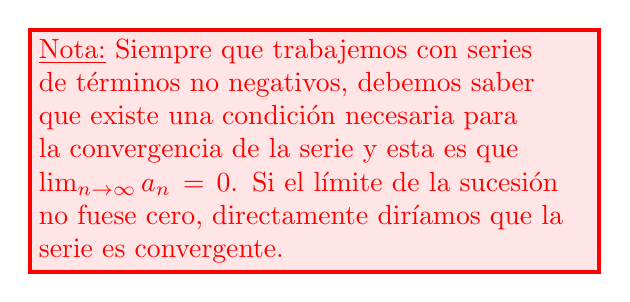
\begin{tikzpicture}[baseline=(current bounding box.center)]
            \node[red,draw=red,fill=red!10,line width=1.5pt,text width=7cm] {\underline{Nota:} Siempre que trabajemos con series de términos no negativos, debemos saber que existe una condición necesaria para la convergencia de la serie y esta es que $\lim_{n\to\infty}a_n=0$. Si el límite de la sucesión no fuese cero, directamente diríamos que la serie es convergente.};
      \end{tikzpicture}
\end{minipage}
\item \lb{Estudiar la convergencia de las serie:}

$\db{\sum_{n=2}^{\infty}\dfrac{1}{\left(\log(n)\right)^n}}$

Para estudiar la convergencia de esta serie, aplicaremos el criterio de la raíz: \begin{center}
      $\lim_{n\to\infty}\sqrt[\cancel{n}]{\dfrac{1}{\left(\log(n)\right)^{\cancel{n}}}}=\lim_{n\to\infty}\dfrac{1}{\log(n)}=\dfrac{1}{\infty}=0<1\quad$ La serie es convergente. 
\end{center}
\item \lb{Estudiar la convergencia de las series}

\begin{minipage}[l]{0.6\linewidth}
      $\db{\sum_{n=1}^{\infty}\dfrac{(n+1)!-n!}{4^n}=}\sum_{n=1}^{\infty}\dfrac{(n+1)n!-n!}{4^n}=\sum_{n=1}^{\infty}\dfrac{n!(n+\cancel{1}-\cancel{1})}{4^n}=\sum_{n=1}^{\infty}\dfrac{n!\cdot n}{4^n}$\\
      Al haber una factorial en la serie, lo que vamos a hacer para estudiar el carácter de convergencia es aplicar el criterio del cociente.  \begin{center}
            $\lim_{n\to\infty}\dfrac{a_{n+1}}{a_n}=\lim_{n\to\infty}\dfrac{\frac{(n+1)!\cdot(n+1)}{4^{n+1}}}{\frac{n!\cdot n}{4^n}}=\lim_{n\to\infty}\dfrac{(n+1)\cdot\cancel{n!}(n+1)\cdot\cancel{4^n}}{\cancel{4^n}\cdot4\cdot\cancel{n!}\cdot n}=\lim_{n\to\infty}\dfrac{n^2+2n+1}{4n}=\lim_{n\to\infty}\left(\cancelto{+\infty}{\dfrac{n}{4}}+\dfrac{1}{2}+\tozero{\dfrac{1}{4^n}}\right)=+\infty>1\quad$ 
      \end{center}La serie es divergente.
\end{minipage}\qquad
\begin{minipage}[l]{0.4\linewidth}
      
\begin{tikzpicture}[baseline=(current bounding box.center)]
            \node[red,draw=red,fill=red!10,line width=1.5pt,text width=6cm] {\underline{Nota:} El criterio del cociente lo aplicaremos fundamentalmente cuando tengamos un factorial o un cociente entre un polinomio y uno exponencial.};
      \end{tikzpicture}
\end{minipage}
\item \lb{Estudiar la convergencia de las series:}

$\db{\sum_{n=1}^{\infty}(n+1)^ne^{-n^2}=}\sum_{n=1}^{\infty}\dfrac{(n+1)^n}{e^{-n^2}}=\sum_{n=1}^{\infty}\left(\dfrac{n+1}{e^n}\right)^n$

Para estudiar la convergencia, lo que haremos será aplicar el criterio de la raíz: \[ \begin{aligned}
      \lim_{n\to\infty}\sqrt[\cancel{n}]{\left(\dfrac{n+1}{e^n}\right)^{\cancel{n}}}=\lim_{n\to\infty}\dfrac{n+1}{e^n}=\left(\dfrac{\infty}{\infty}\right)=\{\mathrm{Stolz}\}&=\lim_{n\to\infty}\dfrac{(\cancel{n}+2)-(\cancel{n}+1)}{e^{n+1}-e^n}=\lim_{n\to\infty}\dfrac{1}{e^n\cdot e-e^n}\\
      &=\lim_{n\to\infty}\dfrac{1}{e^n(e-1)}=\dfrac{1}{\infty}=0<1
\end{aligned} \] La serie es convergente.
\item \lb{Demostrar la convergencia y hallar la suma de las series:}

$\db{\sum_{n=1}^{\infty}\dfrac{2n}{3^n}}$

\begin{minipage}[l]{0.5\textwidth}
      Lo primero que vamos a hacer es comprobar si la serie es convergente o no, y para ello, como es el cociente entre un polinomio y una exponencial aplicaremos el criterio del cociente: 
      
      $\lim_{n\to\infty}\dfrac{a_{n+1}}{a_n}=\lim_{n\to\infty}\dfrac{\frac{2(n+1)}{3^{n+1}}}{\frac{2n}{3^n}}=\lim_{n\to\infty}\dfrac{(2n+2)\cdot\cancel{3^n}}{2n\cdot\cancel{3^n}\cdot3}=\lim_{n\to\infty}\dfrac{2n+2}{6n}=\lim_{n\to\infty}\left(\dfrac{2n}{6n}+\tozero{\dfrac{2}{6n}}\right)=\dfrac{1}{3}<1 $ 
      
      La serie es convergente.
      
      Para sumar la serie debemos darnos cuenta de que estamos ante una serie aritmético-geométrica: 
      
      $\sum_{n=1}^{\infty}\dfrac{2n}{3^n}=\sum_{n=1}^{\infty}2n\cdot\left(\dfrac{1}{3}\right)^{n}=\sum_{n=1}^{\infty}a_nb_n=\lim_{n\to\infty}\underset{\lb{S_n}}{\bboxed{\sum_{j=1}^{n}a_jb_j}}=\lb{(\ast)}$
\end{minipage}\qquad
\begin{minipage}[l]{0.4\textwidth}
      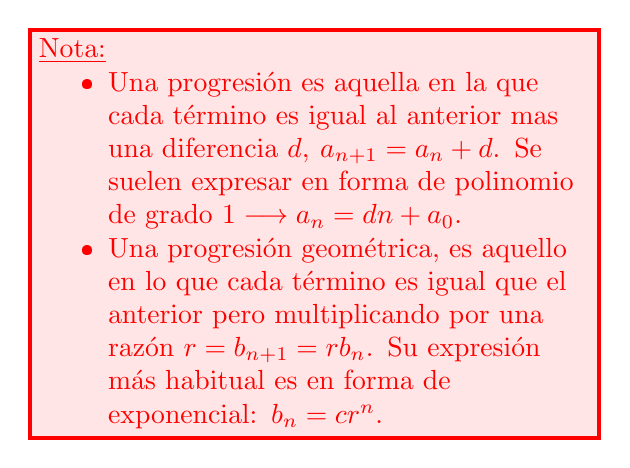
\begin{tikzpicture}[baseline=(current bounding box.center)]
            \node[red,draw=red,fill=red!10,line width=1.5pt,text width=7cm] {\underline{Nota:} \begin{itemize}
                        \item Una progresión es aquella en la que cada término es igual al anterior mas una diferencia $d,\:a_{n+1}=a_n+d$. Se suelen expresar en forma de polinomio de grado $1\longrightarrow a_n=dn+a_0$.
                        \item Una progresión geométrica, es aquello en lo que cada término es igual que el anterior pero multiplicando por una razón $r=b_{n+1}=rb_n$. Su expresión más habitual es en forma de exponencial: $b_n=cr^n$.
            \end{itemize}};
      \end{tikzpicture}
\end{minipage}

\begin{minipage}[l]{0.3\linewidth}
      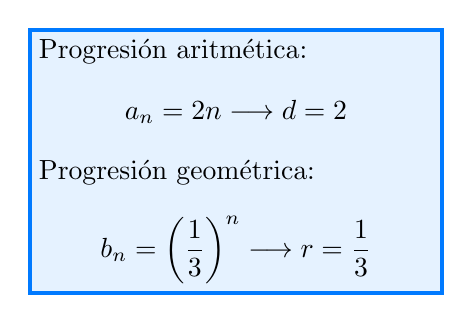
\begin{tikzpicture}[baseline=(current bounding box.center)]
            \node[draw=lightblue,fill=lightblue!10,line width=1.5pt,text width=5cm] {Progresión aritmética: $$a_n=2n\longrightarrow d=2$$\\
            Progresión geométrica: $$b_n=\left(\dfrac{1}{3}\right)^n\longrightarrow r=\dfrac{1}{3}$$};
      \end{tikzpicture}
\end{minipage}

$\begin{array}{l}
      \begin{array}{lcl}
S_n=a_1b_1&+&a_2b_2+a_3b_3+a_4b_4+\cdots+a_nb_n\\
rS_n= & -&a_1b_2-a_2b_3-a_3b_4-\cdots-a_{n-1}b_n-a_nb_{n+1}\\ \hline
\multicolumn{3}{l}{\text{\underline{resto} }(1-r)S_n=a_1b_1+b_2\lbb{(a_2-a_)}{d}+b_3\lbb{(a_3-a_2)}{d}+b_4\lbb{(a_4-a_3)}{d}+\cdots+b_n\lbb{(a_n-a_{n-1})}{d}-a_nb_{n+1}}
\end{array}\\
(1-r)S_n=a_1b_1+d\underset{\lb{\frac{b_2-b_nr}{1-r}}}{[b_2+b_3+b_4+\cdots+b_n]}-a_nb_{n+1}\longrightarrow (1-r)S_n=a_1b_1+d\left(\dfrac{b_2-b_nr}{1-r}\right)-a_nb_{n+1}\\
\bboxed{S_n=\dfrac{a_1b_1}{1-r}+d\dfrac{b_2-b_nr}{(1-r)^2}-\dfrac{a_nb_{n+1}}{1-r}}\\
\begin{aligned}
      \lb{(\ast)=}\lim_{n\to\infty}\left(\dfrac{a_1b-1}{1-r}+d\dfrac{b_2-b_nr}{(1-r)^2}-\dfrac{a_nb_{n+1}}{1-r}\right)&=\lim_{n\to\infty}\left(\dfrac{2\cdot\frac{1}{3}}{1-\frac{1}{3}}+2\cdot\dfrac{\left(\frac{1}{3}\right)^2-\tozero{\left(\frac{1}{3}\right)^n\cdot\frac{1}{3}}}{\left(1-\frac{1}{3}\right)^2}-\tozero{\dfrac{2n\left(\frac{1}{3}\right)^{n+1=\left(\frac{1}{3}\right)^n\cdot\frac{1}{3}}}{1-\frac{1}{3}}}\right)\\
      &=\lb{(\ast\ast)}
\end{aligned}
\end{array}$

Tomamos: $\lim_{n\to\infty}\dfrac{2n}{3^n}=\left(\dfrac{\infty}{\infty}\right)=\{\mathrm{Stolz}\}=\lim_{n\to\infty}\dfrac{2(n+1)-2n}{3^{n+1}-3^n}=\lim_{n\to\infty}\dfrac{2}{3^n(3-1)=\lim_{n\to\infty}\dfrac{1}{3^n}=0}$

$\lb{(\ast\ast)=}\dfrac{\frac{2}{3}}{\frac{2}{3}}+2\cdot\dfrac{\frac{1}{9}}{\frac{4}{9}}=1+\dfrac{1}{2}=\dfrac{3}{2}$

Por lo tanto, tenemos que: $\bboxed{\sum_{n=1}^{\infty}\dfrac{2n}{3^n}=\dfrac{3}{2}}$
\item \lb{Demostrar la convergencia y hallar la suma de las series:}

$\db{\sum_{n=1}^{\infty}\dfrac{4n+2}{3^n}}$

\begin{minipage}[l]{0.45\linewidth}
Para estudiar la convergencia, al tener un polinomio con una exponencial, lo que haremos será aplicar el criterio del cociente:

$\lim_{n\to\infty}\dfrac{a_{n+1}}{a_n}=\lim_{n\to\infty}\dfrac{\frac{4(n+1)-2}{3^{n+1}}}{\frac{4n+2}{2^n}}=\lim_{n\to\infty}\dfrac{(4n+6)\cdot\cancel{3^n}}{(4n+2)\cdot\cancel{3^n}\cdot3}=\lim_{n\to\infty}\dfrac{4n+6}{12n+6}=\left(\dfrac{\infty}{\infty}\right)=\lim_{n\to\infty}\dfrac{\frac{4n}{n}+\tozero{\frac{6}{n}}}{\frac{12n}{n}+\tozero{\frac{6}{n}}}=\dfrac{4}{12}=\dfrac{1}{3}<1$ \fcolorbox{lightblue}{lightblue!10}{La serie es convergente}

\end{minipage}\qquad
\begin{minipage}[l]{0.5\linewidth}
      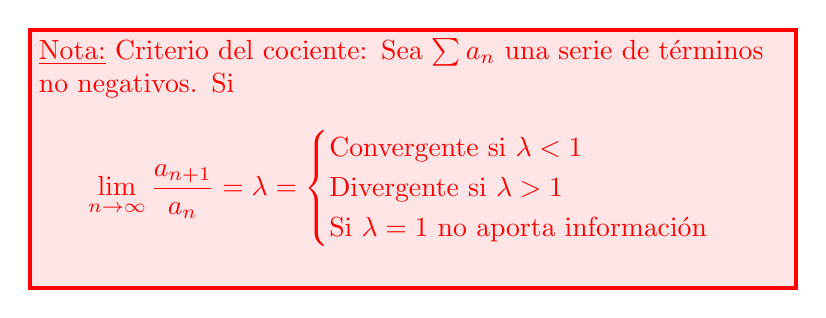
\begin{tikzpicture}[baseline=(current bounding box.center)]
            \node[red,draw=red,fill=red!10,line width=1.5pt,text width=9.5cm] {\underline{Nota:} Criterio del cociente: Sea $\sum a_n$ una serie de términos no negativos. Si \[ \lim_{n\to\infty}\dfrac{a_{n+1}}{a_n}=\lambda=\begin{cases}
                        \text{Convergente si }\lambda<1\\
                        \text{Divergente si }\lambda>1\\
                        \text{Si $\lambda=1$ no aporta información}
                  \end{cases} \]};
      \end{tikzpicture}
\end{minipage}

Para sumar la serie debemos darnos cuenta que estamos ante una serie aritmético-geométrica, es decir:
\begin{itemize}
      \item Progresión aritmética: $a_n=4n+2\longrightarrow d=a_2-a_1=4$.
      \item Progresión geométrica: $b_n=\left(\dfrac{1}{3}\right)^n\longrightarrow r=\dfrac{b_2}{b_1}=\dfrac{1}{3}$.
\end{itemize}
$\begin{array}{l}
      \sum_{n=1}^{\infty}\dfrac{4n+2}{3^n}=\sum_{n=1}^{\infty}(4n+2)\left(\dfrac{1}{3}\right)^n=\sum_{n=1}^{\infty}a_nb_n=\lim_{n\to\infty}\lbb{\sum_{j=1}^{n}a_jb_j}{S_n}\\
      \begin{array}{ll}
      S_n=a_1b_1+&a_2+b_2+a_3b_3+a_4b_4+\cdots+a_nb_n\\
      rS_n= & a_1b_2+a_2b_3+a_3b_4+\cdots+a_{n-1}b_n+a_nb_{n+1}\\ \hline
      \multicolumn{2}{l}{\text{\underline{resto} }(1-r)S_n=a_1b_1+\lbb{(a_2-a_1)}{d}b_2+\lbb{(a_3-a_2)}{d}b_3+\lbb{(a_4-a_3)}{d}b_4+\cdots+\lbb{(a_n-a_{n+1})}{d}b_n-a_nb_{n+1}}
\end{array}\\
(1-r)S_n=a_1b_1+d\underset{\lb{\dfrac{b_2-b_nr}{1-r}}}{[b_2+b_3+b_4+\cdots+b_n]}-a_nb_{n+1}\\
(1-r)S_n=a_1b_1+d\left(\dfrac{b_2-b_nr}{1-r}\right)-a_nb_{b+1}\longrightarrow\bboxed{S_n=\dfrac{a_1b_1}{1-r}+d\dfrac{b_2-b_nr}{(1-r)^2}-\dfrac{a_nb_{n+1}}{1-r}}\\
\begin{aligned}
      \sum_{n=1}^{\infty}\dfrac{4n+2}{3^n}&=\sum_{n=1}^{\infty}(4n+2)\left(\dfrac{1}{3}\right)^n=\sum_{n=1}^{\infty}a_nb_n=\lim_{n\to\infty}\lbb{\sum_{j=1}^{n}a_jb_j}{S_n}=\lim_{n\to\infty}\left[\dfrac{a_1b_1}{1-r}+d\dfrac{b_2-b_nr}{(1-r)^2}-\dfrac{a_nb_{n+1}}{1-r}\right]\\
&=\lim_{n\to\infty}\left[\dfrac{6\cdot\left(\frac{1}{3}\right)}{1-\frac{1}{3}}+4\cdot\dfrac{\left(\frac{1}{3}\right)^2}-\tozero{\left(\frac{1}{3}\right)^n\cdot\left(\frac{1}{3}\right)}{\left(1-\frac{1}{3}\right)^2}-\tozero{\dfrac{(4n+2)\cdot\left(\frac{1}{3}\right)^{n+1}}{1-\frac{1}{3}}}\right]\\
&=\dfrac{2}{\frac{2}{3}}+\dfrac{\frac{4}{9}}{\frac{4}{9}}=3+1=\bboxed{4}
\end{aligned}
\end{array}$
\item \lb{Hallar la suma de las series:}

$\db{\sum_{n=0}^{\infty}\dfrac{(-1)^n}{5^n}}$

\begin{minipage}[l]{0.45\textwidth}
      Como en este caso hay términos negativos y positivos, lo que vamos a hacer es comprobar si es absolutamente convergente: \[ \sum_{n=0}^{\infty}\left|\dfrac{(-1)^n}{5^n}\right|=\sum_{n=0}^{\infty}\dfrac{1}{5^n} \] Para estudiar la convergencia de esta serie aplicaremos el criterio de la raíz:  \begin{center}
            $\lim_{n\to\infty}\sqrt[\cancel{n}]{\left(\dfrac{1}{5}\right)^{\cancel{n}}}=\dfrac{1}{5}<1\longrightarrow$\fcolorbox{lightblue}{lightblue!10}{La serie es convergente}
      \end{center}
      Para sumar esta serie debemos escribirla como: 
\end{minipage}\qquad
\begin{minipage}[l]{0.6\textwidth}
      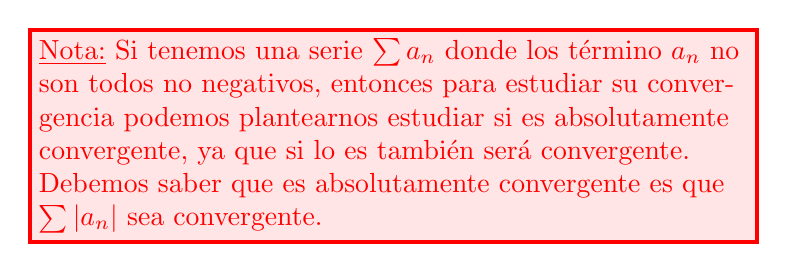
\begin{tikzpicture}[baseline=(current bounding box.center)]
            \node[red,draw=red,fill=red!10,line width=1.5pt,text width=9cm] {\underline{Nota:} Si tenemos una serie $\sum a_n$ donde los término $a_n$ no son todos no negativos, entonces para estudiar su convergencia podemos plantearnos estudiar si es absolutamente convergente, ya que si lo es también será convergente. Debemos saber que es absolutamente convergente es que $\sum|a_n|$ sea convergente.};
      \end{tikzpicture}
\end{minipage}
\[ \sum_{n=0}^{\infty}\dfrac{(-1)^n}{5^n}=\sum_{n=0}^{\infty}\left(\dfrac{-1}{5}\right)^n=\sum_{n=0}^{\infty}b_n=\lim_{n\to\infty}\lbb{\sum_{j=0}^{n}b_j}{S_n}=\lb{(\ast)}=\lim_{n\to\infty}\dfrac{b_0-b_{n+1}}{1-r}=\lim_{n\to\infty}\dfrac{1-\tozero{\left(\frac{-1}{5}\right)^{n+1}}}{1-\left(-\frac{1}{5}\right)}=\dfrac{1}{\frac{6}{5}}=\bboxed{\dfrac{5}{6}} \]
$\lb{(\ast)}\qquad\begin{array}{l|l|l}
      S_n=b_0 & \bcancel{+b_1+b_2+b_3+\cdots+b_n} & \\
      rS_n= & \bcancel{-b_1-b_2-b_3-\cdots-b_n}&-b_{n+1}\\ \hline
      \multicolumn{3}{l}{\text{\underline{resto} }(1-r)S_n=b_0-b_{n+1}\longrightarrow\bboxed{S_n=\dfrac{b_0-b_{n+1}}{1-r}}}
\end{array}$
\item \lb{Demuestre que las siguientes series divergen:}

\begin{minipage}[l]{0.5\textwidth}
      $\db{\sum_{n=1}^{\infty}\left(\dfrac{n+1}{n}\right)^n}$\\
      Como el problema nos pide que demostremos que es divergente, lo primero que vamos a hacer es comprobar si verifica la condición necesaria: \[\lim_{n\to\infty}\left(\dfrac{n+1}{n}\right)^n=(1^\infty)=e^{\lim_{n\to\infty}n\left(\frac{n+1}{n}-1\right)}=\lb{(\ast)}=e^1\neq0  \]Base: $\lim_{n\to\infty}\dfrac{n+1}{n}=\lim_{n\to\infty}\left(1+\dfrac{1}{n}\right)=1$
\end{minipage}\qquad\qquad
\begin{minipage}[l]{0.5\textwidth}
      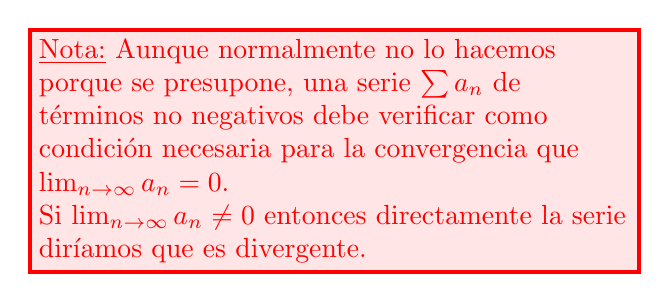
\begin{tikzpicture}[baseline=(current bounding box.center)]
            \node[red,draw=red,fill=red!10,line width=1.5pt,text width=7.5cm] {\underline{Nota:} Aunque normalmente no lo hacemos porque se presupone, una serie $\sum a_n$ de términos no negativos debe verificar como condición necesaria para la convergencia que $\lim_{n\to\infty}a_n=0$.\\
            Si $\lim_{n\to\infty}a_n\neq0$ entonces directamente la serie diríamos que es divergente.};
      \end{tikzpicture}
\end{minipage}

$\lb{(\ast)=}\lim_{n\to\infty}n\left(\dfrac{n+1}{n}-1\right)=\lim_{n\to\infty}n\left(\dfrac{\cancel{n}+1-\cancel{n}}{n}\right)=\lim_{n\to\infty}\dfrac{n}{n}=1$

Como $\lim_{n\to\infty}a_n\neq0\longrightarrow$ La serie es divergente.
\item \lb{Demuestre que las siguientes series divergen:}

$\db{\sum_{n=2}^{\infty}\dfrac{n^{n-2}}{3^n}}$

Como nos piden que demostremos que es divergente, comenzamos comprobando si verifica la condición necesaria para la convergencia \[ \lim_{n\to\infty}a_n=\lim_{n\to\infty}\dfrac{n^{n-2}}{3^n}=\lim_{n\to\infty}\dfrac{n^{n-2}}{3^{n-2}\cdot3^2}=\dfrac{1}{9}\lim_{n\to\infty}\left(\dfrac{n}{3}\right)^{n-2}=\infty^\infty=\infty\neq0 \]Como $\lim_{n\to\infty}a_n\neq0$ entonces al no cumplirse la condición necesaria diremos que $\sum_{n=2}^{\infty}\dfrac{n^{n-2}}{3^n}$ es divergente.
\item \lb{Estudiar la convergencia y la convergencia absoluta de las series:}

\begin{minipage}[l]{0.5\textwidth}
      Comenzamos estudiando la convergencia absoluta: \begin{center}
            $\sum_{n=1}^{\infty}\left|\dfrac{(-1)^n}{n^2}\right|=\sum_{n=1}^{\infty}\dfrac{1}{n^2}$ esta serie es la armónica generalizada con $p=2>1$ es convergente.
      \end{center}Por lo tanto $\sum_{n=1}^{\infty}\dfrac{(-1)^n}{n^2}$ es absolutamente convergente $\longrightarrow$ también es convergente.
\end{minipage}\qquad
\begin{minipage}[l]{0.5\textwidth}
      
\begin{tikzpicture}[baseline=(current bounding box.center)]
            \node[red,draw=red,fill=red!10,line width=1.5pt,text width=7cm] {\underline{Nota:} Siempre que nos pidan que estudiemos la convergencia y la convergencia absoluta, ya que en caso de ser absolutamente convergente, automáticamente sería convergente. En caso de no ser absolutamente convergente entonces estudiaremos la convergencia.};
      \end{tikzpicture}
\end{minipage}
\item \lb{Determinar el dominio de definición de las siguientes funciones:}

$\db{f(x)=x-\sqrt{\dfrac{x+2}{x-1}}}$
\begin{itemize}
      \item Como tenemos un cociente, su denominador no puede ser cero: \[ \bboxed{x=1}\notin\mathrm{Dom}(f) \]
      \item Como tenemos una raíz cuadrada, lo de dentro de ser positivo o cero: \begin{center}
            $\dfrac{x+2}{x-1}\ge0\longrightarrow\qquad$
            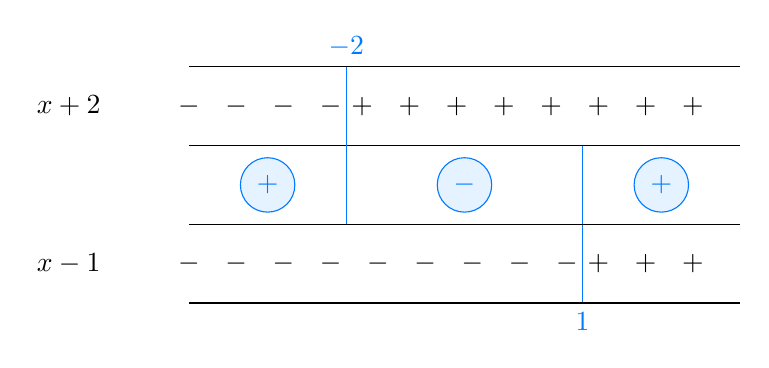
\begin{tikzpicture}[baseline=(current bounding box.center)]
                  \draw (-4,0) -- (3,0);
                  \draw (-4,1) -- (3,1);
                  \foreach \x in {-4,-3.4,...,-2}{
                  \node at (\x,0.5) {$-$};
                  }
                  \foreach \x in {-1.8,-1.2,...,3}{
                        \node at (\x,0.5) {$+$};
                  }
                  \foreach \x in {-4,-3.4,...,1}{
                        \node at (\x,-1.5) {$-$};
                  }
                  \foreach \x in {1.2,1.8,...,3}{
                        \node at (\x,-1.5) {$+$};
                  }
                  \node[circle, draw=lightblue, fill=lightblue!10] at (-3,-0.5) {$\lb{+}$};
                  \node[circle, draw=lightblue, fill=lightblue!10] at (2,-0.5) {$\lb{+}$};
                  \node[circle, draw=lightblue, fill=lightblue!10] at (-0.5,-0.5) {$\lb{-}$};
                  \draw[lightblue] (-2,1) node[above] {$-2$} -- (-2,-1);
                  \draw[lightblue] (1,0)  -- (1,-2) node[below] {$1$};
                  \draw (-4,-1) -- (3,-1);
                  \draw (-4,-2) -- (3,-2);
                  \node[left] at (-5,0.5) {$x+2$};
                  \node[left] at (-5,-1.5) {$x-1$};
            \end{tikzpicture}
      \end{center}
\end{itemize}
$\bboxed{\mathrm{Dom}(f)=(-\infty,-2]\cup(1,+\infty)}$
\item \lb{Determinar el dominio de definición de las siguientes funciones:}

$\db{f(x)=\sqrt[4]{\dfrac{x}{\log(x)}}}$
\begin{itemize}
      \item Como tenemos un logaritmo, entonces debe verificarse que lo de dentro del logaritmo sea mayor estricto que cero: \[ \bboxed{x>0} \]
      \item Como tenemos un cociente, este debe verificar que si denominador no sea cero \[ \log(x)=0\longrightarrow\bboxed{x=1}\notin\mathrm{Dom}(f) \]
      \item Como tenemos una raíz de grado para entonces su valor no puede ser negativo.\begin{center}
            $\dfrac{x}{\log(x)\ge0}\qquad$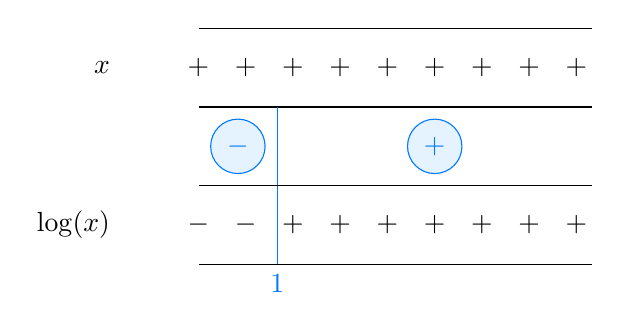
\begin{tikzpicture}[baseline=(current bounding box.center)]
                  \draw (0,0) -- (5,0);
                  \draw (0,1) -- (5,1);
                  \foreach \x in {0,0.6,...,5}{
                        \node at (\x,0.5) {$+$};
                  }
                  \foreach \x in {0,0.6,...,1}{
                        \node at (\x,-1.5) {$-$};
                  }
                  \foreach \x in {1.2,1.8,...,5}{
                        \node at (\x,-1.5) {$+$};
                  }
                  \node[circle, draw=lightblue, fill=lightblue!10] at (3,-0.5) {$\lb{+}$};
                  \node[circle, draw=lightblue, fill=lightblue!10] at (0.5,-0.5) {$\lb{-}$};
                  \draw[lightblue] (1,0)  -- (1,-2) node[below] {$1$};
                  \draw (0,-1) -- (5,-1);
                  \draw (0,-2) -- (5,-2);
                  \node[left] at (-1,0.5) {$x$};
                  \node[left] at (-1,-1.5) {$\log(x)$};
            \end{tikzpicture}
            \end{center}
\end{itemize}
$\bboxed{\mathrm{Dom}(f)=(1,+\infty)}$
\item \lb{Dadas las siguientes funciones, averiguar en qué puntos son discontinuas y por qué.}

$\db{f(x)=\dfrac{x^2}{x-2}\text{ si }x\neq2,\:f(2)=0}$

$f(x)=\begin{cases}
      \dfrac{x^2}{x-2}& \text{si }x\neq2\\
      0 & \text{si }x=2
\end{cases}$

$\forall\:x\neq2\longrightarrow f(x)$ es continua por ser un cociente de funciones continuas con denominador distinto de cero.

\bu{Veamos que pasa en $x=2$:}

$\lim_{x\to2}\dfrac{x^2}{x-2}=\dfrac{4}{0}=\{\text{Tenemos que distinguir en los límites laterales}\}=\begin{cases}
      \lim_{x\to2^-}\dfrac{x^2}{x-2}=\dfrac{2^2}{0^-}=-\infty\\
      \lim_{x\to2^+}\dfrac{x^2}{x-2}=\dfrac{4}{0^+}=+\infty
\end{cases}$

Por lo tanto $f(x)$ no es continua en $x=2$, en concreto presenta en $x=2$ una discontinuidad inevitable de salto infinito. Diremos que $f(x)$ tiene en $x=2$ una asintótica vertical.
\item \lb{Calcular los siguientes límites:}

$\begin{array}{l}
      \db{\lim_{x\to2}\dfrac{x^2-2x}{x^2-4x+4}=}\left(\dfrac{0}{0}\right)=\lim_{x\to2}\dfrac{x\cancel{(x-2)}}{(x-2)^{\cancel{2}}}=\lim_{x\to2}\dfrac{x}{x-2}=\left(\dfrac{2}{0}\right)=\begin{cases}
      \lim_{x\to2^-}\dfrac{x}{x-2}=\dfrac{2}{0^-}=-\infty\\
      \lim_{x\to2^+}\dfrac{x}{x-2}=\dfrac{2}{0^+}=+\infty
\end{cases}\nexists\lim\\
x^2-2x=x(x-2)\\
x^2-4x+4=(x-2)^2
\end{array}$
\item \lb{Calcular los siguientes límites:}

\begin{minipage}[l]{0.6\textwidth}
      $\db{\lim_{x\to a}\dfrac{\sqrt{x}-\sqrt{a}}{x-a}=}\left(\dfrac{0}{0}\right)=\lim_{x\to a}\dfrac{(\sqrt{x}-\sqrt{a})(\sqrt{x}+\sqrt{a})}{(x-a)(\sqrt{x}-\sqrt{a})}=\lim_{x\to a}\dfrac{\cancel{x-a}}{\cancel{(x-a)}(\sqrt{x}+\sqrt{a})}=\lim_{x\to a}=\dfrac{1}{\sqrt{x}+\sqrt{a}}=\bboxed{\dfrac{1}{2\sqrt{a}}}$
\end{minipage}\qquad
\begin{minipage}[l]{0.4\textwidth}
      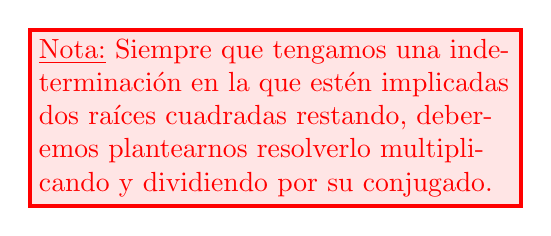
\begin{tikzpicture}[baseline=(current bounding box.center)]
            \node[red,draw=red,fill=red!10,line width=1.5pt,text width=6cm] {\underline{Nota:} Siempre que tengamos una indeterminación en la que estén implicadas dos raíces cuadradas restando, deberemos plantearnos resolverlo multiplicando y dividiendo por su conjugado.};
      \end{tikzpicture}
\end{minipage}
\item \lb{Calcular el siguiente límite: \[ \lim_{n\to\infty}(\sqrt{x^2+4}-\sqrt{x^2-1}) \]}

$\begin{aligned}
      \lim_{n\to\infty}(\sqrt{x^2+4}-\sqrt{x^2-1})&=(\infty-\infty)=\lim_{n\to\infty}\dfrac{(\sqrt{x^2+4}-\sqrt{x^2-1})(\sqrt{x^2+4}+\sqrt{x^2-1})}{\sqrt{x^2+4}+\sqrt{x^2-1}}\\
      &=\lim_{n\to\infty}\dfrac{(\cancel{x^2}+4)-(\cancel{x^2}-1)}{\sqrt{x^2+4}+\sqrt{x^2-1}}=\lim_{n\to\infty}\dfrac{5}{\sqrt{x^2+4}+\sqrt{x^2-1}}=\dfrac{4}{\infty}=\bboxed{0}
\end{aligned}$
\item \lb{Calcular los siguientes límites ordinarios o laterales:}

      $\db{\lim_{x\to1}\dfrac{x^{\frac{1}{3}}-1}{x-1}=}\lim_{x\to1}\dfrac{\sqrt[3]{x}-1}{x-1}=\left(\dfrac{0}{0}\right)=\lb{(\ast)}$
      
      $\begin{array}{l}
            \sqrt[3]{x-1}=b-a=\dfrac{x-1}{\sqrt[3]{x^2}+\sqrt[3]{x}+1}\\
            b=\sqrt[3]{x}\\
            a=1\\
            b^3-a^3=(b-a)(b^2-ab+a^2)\longrightarrow\bboxed{b-a=\dfrac{b^3-a^3}{b^2+ba+a^2}}\\
            \lb{(\ast)=}\lim_{x\to1}\dfrac{\frac{\cancel{x-1}}{\sqrt[3]{x^2}+\sqrt[3]{x}+1}}{x-1}=\lim_{x\to1}\dfrac{1}{\sqrt[3]{x^2}+\sqrt[3]{x}+1}=\bboxed{\dfrac{1}{3}}
      \end{array}$

\begin{minipage}[l]{0.5\textwidth}
      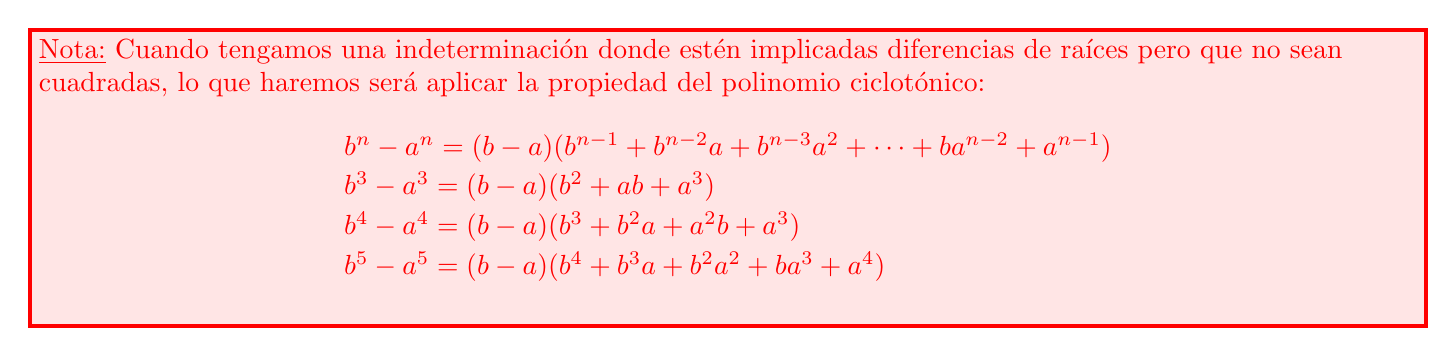
\begin{tikzpicture}[baseline=(current bounding box.center)]
            \node[red,draw=red,fill=red!10,line width=1.5pt,text width=17.5cm] {\underline{Nota:} Cuando tengamos una indeterminación donde estén implicadas diferencias de raíces pero que no sean cuadradas, lo que haremos será aplicar la propiedad del polinomio ciclotónico: \[ \begin{array}{l}
                        b^n-a^n=(b-a)(b^{n-1}+b^{n-2}a+b^{n-3}a^2+\cdots+ba^{n-2}+a^{n-1})\\
                        b^3-a^3=(b-a)(b^2+ab+a^3)\\
                        b^4-a^4=(b-a)(b^3+b^2a+a^2b+a^3)\\
                        b^5-a^5=(b-a)(b^4+b^3a+b^2a^2+ba^3+a^4)
                  \end{array} \]};
      \end{tikzpicture}
\end{minipage}
\item \lb{Calcular los siguientes límites ordinarios o laterales:}

$\begin{array}{l}
      \db{\lim_{x\to+\infty}\left(\sqrt[3]{x^2+1}-x\right)=}(\infty-\infty)=\lim_{x\to+\infty}\dfrac{1}{\sqrt[3]{(x^3+1)^2}+x\sqrt[3]{x^3+1}+x^2}=\dfrac{1}{\infty}=\bboxed{0}\\
      \sqrt[3]{x^3+1}-x=b-a=\dfrac{b^3-a^3}{b^2+ab+a^2}=\dfrac{\cancel{x^3}+1-\cancel{x^3}}{\sqrt[3]{(x^3+1)^2}+x\sqrt[3]{x^3+1}+x^2}=\dfrac{1}{\sqrt[3]{(x^3+1)^2}+x\sqrt[3]{x^3+1}+x^2}\\
      b^3-a^3=(b-a)(b^2+ab+a^2)
\end{array}$
\item \lb{Calcular los siguientes límites:}

$\begin{array}{l}
      \db{\lim_{x\to a}\dfrac{x^2-(a+1)x+a}{x^3-a^3}}=\left(\dfrac{0}{0}\right)=\lim_{x\to a}\dfrac{\cancel{(x-a)}(x-1)}{\cancel{(x-a)}(x^2+xa+a^2)}=\bboxed{\dfrac{a-1}{3a^2}}\\
      x^2-(a+1)x+a=\lbb{x^2-ax}{}-\dbb{x+a}{}=\lbb{x(x-a)}{}-(x-a)=(x-a)(x-1)\\
      x^3-a^3=(x-a)(x^2+x\cdot a +a^2)
\end{array}$
\item \lb{Calcule el límite (si es posible) de $\lim_{x\to0}\dfrac{f(x)}{|x|}$ sabiendo que $\lim_{x\to0}xf(x)=3$}

$\begin{array}{l}
      \lim_{x\to 0}\dfrac{f(x)}{|x|}=\begin{cases}
            \lim_{x\to0^-}\dfrac{f(x)}{-x}=-\lim_{x\to0^-}\dfrac{xf(x)}{x^2}=-\dfrac{3}{0^+}=-\infty\\
            \lim_{x\to0^+}\dfrac{f(x)}{x}=\lim_{x\to0^+}\dfrac{xf(x)}{x^2}=\dfrac{3}{0^+}=+\infty\\
      \end{cases}\\
      |x|=\begin{cases}
            x & \text{si }x\ge0\\
            -x & \text{si }g<0
      \end{cases}
\end{array}$

\item \lb{Calcular el siguiente límite: \[ \lim_{x\to 0}\dfrac{\sin(x)}{x} \]}

$\lim_{x\to 0}\dfrac{\sin(x)}{x}=\left(\dfrac{0}{0}\right)=\left\{\sin(x)\leadsto_0x\right\}=\lim_{x\to0}\dfrac{x}{x}=\bboxed{1}\qquad$
\begin{minipage}[l]{0.5\textwidth}
            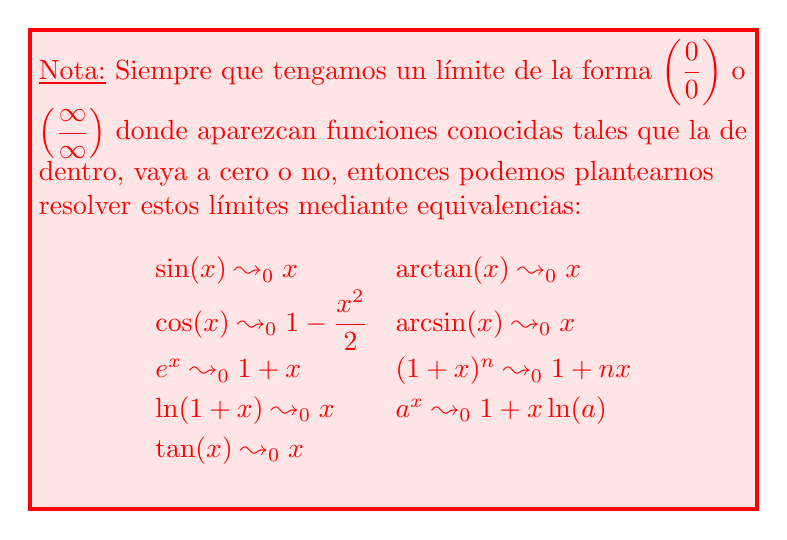
\begin{tikzpicture}[baseline=(current bounding box.center)]
            \node[red,draw=red,fill=red!10,line width=1.5pt,text width=9cm] {\underline{Nota:} Siempre que tengamos un límite de la forma $\left(\dfrac{0}{0}\right)$ o $\left(\dfrac{\infty}{\infty}\right)$ donde aparezcan funciones conocidas tales que la de dentro, vaya a cero o no, entonces podemos plantearnos resolver estos límites mediante equivalencias: \[ \begin{array}{ll}
                        \sin(x)\leadsto_0x & \arctan(x)\leadsto_0x\\
                        \cos(x)\leadsto_01-\dfrac{x^2}{2} & \arcsin(x)\leadsto_0x\\
                        e^x\leadsto_01+x & (1+x)^n\leadsto_01+nx\\
                        \ln(1+x)\leadsto_0x & a^x\leadsto_01+x\ln(a) \\
                        \tan(x)\leadsto_0x & 
                  \end{array} \]};
      \end{tikzpicture}
\end{minipage}
\item \lb{Calcular los siguientes límites:}

$\db{\lim_{x\to0}\dfrac{x^2\cdot(1-\cos(x))}{\sin^4(x)}=}\left(\dfrac{0}{0}\right)=\left\{\begin{array}{l}
      \text{Equivalencias}\\
      \cos(x)\leadsto_01-\dfrac{x^2}{2}\\
      \sin(x)\leadsto_0x
\end{array}\right\}=\lim_{x\to0}\dfrac{x^2\cdot\left(\cancel{1}-\left(\cancel{1}-\frac{x^2}{2}\right)\right)}{x^4}=\lim_{x\to0}\dfrac{\frac{x^4}{2}}{x^4}=\bboxed{\dfrac{1}{2}}$

\item \lb{Calcular los siguientes límites:}

$\db{\lim_{x\to0}\dfrac{1-\cos(ax)}{x(2-x)\tan(bx)}=}\left(\dfrac{0}{0}\right)=\lb{(\ast)}$

Aplicaremos equivalencias:

$\begin{array}{l}
      \cos(x)\leadsto_01-\dfrac{x^2}{2}\longrightarrow\cos(ax)\leadsto_01-\dfrac{(ax)^2}{2}=1-\dfrac{a^2x^2}{2}\\
      \tan(x)\leadsto_0x\longrightarrow\tan(bx)\leadsto_0bx\\
      \lb{(\ast)=}\lim_{x\to0}\dfrac{\cancel{1}-\left[\cancel{1}-\frac{a^2x^2}{2}\right]}{x(2-x)\cdot bx}=\lim_{x\to0}\dfrac{\frac{a^2}{2}x^2}{x(2-x)\cdot bx}=\lim_{x\to0}\dfrac{\frac{a^2}{2}x^2}{x(2-x)bx}=\lim_{x\to0}\dfrac{\frac{a^2}{2}\cancel{x^2}}{b\cancel{x^2}(2-x)}=\lim_{x\to0}\dfrac{\frac{a^2}{2}}{b(2-x)}=\bboxed{\dfrac{a^2}{4b}}
\end{array}$

\item \lb{Calcular los siguientes límites:}

$\begin{aligned}
      \db{\lim_{x\to0}\dfrac{a^x-1}{\sqrt{1+x}-1}=}\left(\dfrac{0}{0}\right)&=\lim_{x\to0}\dfrac{(a^x-1)(\sqrt{1+x}+1)}{(\sqrt{1+x}-1)(\sqrt{1+x}+1)}=\lim_{x\to0}\dfrac{(a^x-1)(\sqrt{1+x}+1)}{\cancel{1}+x-\cancel{1}}\\
      &=\lim_{x\to0}\dfrac{(a^x-1)(\sqrt{1+x}+1)}{x}
      =\left(\dfrac{0}{0}\right)=\left\{\begin{array}{l}
      \text{Equivalencia:}\\
      a^x\leadsto_01+x\ln(a)
\end{array}\right\}\\
&=\lim_{x\to0}\dfrac{(\cancel{1}+x\ln(a)-\cancel{1})(\sqrt{1+x}+1)}{x}=\lim_{x\to0}\dfrac{\cancel{x}(\sqrt{1+x}+1)\ln(a)}{\cancel{x}}=\bboxed{2\ln(a)}
\end{aligned}$

\item \lb{Calcular los siguientes límites}

$\db{\lim_{x\to0}\dfrac{a^x-b^x}{x}=}\left(\dfrac{0}{0}\right)=\left\{\begin{array}{l}
      \text{Equivalencias:}\\
      a^x\leadsto_01+x\ln(a)\\
      b^x\leadsto_01+x\ln(b)
\end{array}\right\}=\lim_{x\to0}\dfrac{(\cancel{1}+x\ln(a))-(\cancel{1}+x\ln(b))}{x}=\lim_{x\to0}\dfrac{\cancel{x}\left[\ln(a)-\ln(b)\right]}{\cancel{x}}=\bboxed{\ln(a)-\ln(b)}$
\item \lb{Calcular los siguiente límites:}

$\begin{array}{l}
      \db{\lim_{x\to1}\left(\dfrac{1}{1-x}-\dfrac{3}{1-x^3}\right)=}\lim_{x\to1}\dfrac{1-x^3-3(1-x)}{(1-x)(1-x^3)}=\lim_{x\to1}\dfrac{-2+3x-x}{(1-x)(1-x^3)}=\left(\dfrac{0}{0}\right)=\lb{(\ast)}\\
      -x^3+3x-2=0\\
      \begin{tabular}{c|cccc}
            & -1 & 0 & 3 & -2 \\
            1 &  & -1 & -1 & 2 \\ \hline
            & -1 & -1 & 2 & \multicolumn{1}{|c|}{0} \\ \cline{5-5}
            1 &  & -1 & 2 &  \\ \hline
            & -1 & -2 & \multicolumn{1}{|c|}{0} &  \\ \cline{4-4}
      \end{tabular} \qquad -x^3+3x-2=(x-1)^2(-x-2)\\
      \begin{cases}
            1-x^3=(1-x)\cdot(1+x+x^2)\\
            a^3-b^3=(a-b)(a^2+ab+b^2)
      \end{cases}\\
      \lb{(\ast)=}\lim_{x\to1}\dfrac{(x-1)^2(-x-2)}{\underset{\begin{subarray}{c}
                  \downarrow\\
                  -(x-1)
      \end{subarray}}{(1-x)}\underset{\begin{subarray}{c}
                  \downarrow\\
                  -(x-1)
      \end{subarray}}{(1-x)}(1+x+x^2)}=\lim_{x\to1}\dfrac{\cancel{(x-1)^2}(-x-2)}{\cancel{(x-1)^2}(1+x+x^2)}=\dfrac{-3}{3}=\bboxed{-1}
\end{array}$
\item \lb{Demostrar la convergencia y hallar la suma de las series:}

$\db{\sum_{n=1}^{\infty}\dfrac{(-2)^n}{3^n}}$

Para estudiar la convergencia, lo que haremos será, realizar el estudio de la convergencia absoluta, ya que si es absolutamente convergente también será convergente.

$\sum_{n=1}^{\infty}\left|\dfrac{(-2)^n}{3^n}\right|=\sum_{n=1}^{\infty}\left(\dfrac{2}{3}\right)^n$ aplicamos el criterio de la raíz: \begin{center}
      $\lim_{n\to\infty}\sqrt[\cancel{n}]{\left(\dfrac{2}{3}\right)^n}=\dfrac{2}{3}<1$ La serie es convergente $\longrightarrow$ Como $\sum_{n=1}^{\infty}\dfrac{(-2)^n}{3^n}$ es absolutamente convergente $\longrightarrow\sum_{n=1}^{\infty}\dfrac{(-2)^n}{3^n}$ es convergente.
\end{center}Para sumar la serie, la tomaremos como $\sum_{n=1}^{\infty}\dfrac{(-2)^n}{3^n}=\sum_{n=1}^{\infty}\left(-\dfrac{2}{3}\right)^n=\sum_{n=1}^{\infty}b_n=\lim_{n\to\infty}\lbb{\sum_{j=1}^{n}b_j}{S_n}=\lb{(\ast)}$

$\begin{array}{l}
      b_n=\left(-\dfrac{2}{3}\right)^n\\
      r=-\dfrac{2}{3}\\
      \begin{array}{l|l|l}
            S_n=b_1 & \bcancel{+b_2+b_3+\cdots+b_n} & \\
            rS_n= & \bcancel{-b_2-b_3-\cdots-b_n} & -b_{n+1}\\ \hline
            \multicolumn{3}{l}{\text{\underline{resto} }(1-r)S_n=b_1-b_{n+1}}\\
      \end{array}\\
      S_n=\dfrac{b_1-b_{n+1}}{1-r}\\
      \lb{(\ast)=}\lim_{n\to\infty}\dfrac{\left(-\frac{2}{3}\right)-\tozero{\left(-\frac{2}{3}\right)^{n+1}}}{1+\frac{2}{3}}=\dfrac{-\frac{2}{3}}{\frac{5}{3}}=\bboxed{-\dfrac{2}{5}}
\end{array}$
\item \lb{Calcular la derivada de $f(x)=x^2$ en un punto genérico $x=x_0$.}

\begin{minipage}[l]{\textwidth}
      \begin{wrapfigure}{r}{0.5\textwidth}
            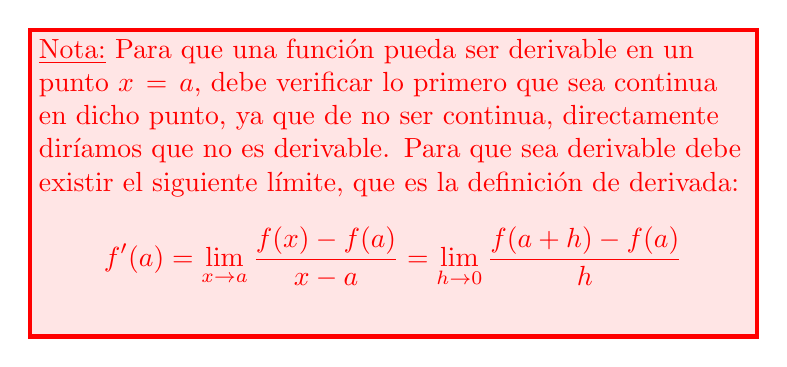
\begin{tikzpicture}[baseline=(current bounding box.center)]
            \node[red,draw=red,fill=red!10,line width=1.5pt,text width=9cm] {\underline{Nota:} Para que una función pueda ser derivable en un punto $x=a$, debe verificar lo primero que sea continua en dicho punto, ya que de no ser continua, directamente diríamos que no es derivable. Para que sea derivable debe existir el siguiente límite, que es la definición de derivada: \[ f'(a)=\lim_{x\to a}\dfrac{f(x)-f(a)}{x-a}=\lim_{h\to0}\dfrac{f(a+h)-f(a)}{h} \]};
      \end{tikzpicture}
      \end{wrapfigure}
      
      Como $f(x)=x^2$ es un polinomio, entonces es siempre continua. 
      
      $f'(x_0)=\lim_{x\to x_0}\dfrac{f(x)-f(x_0)}{x-x_0}=\lim_{x\to x_0}\dfrac{x^2-x_0^2}{x-x_0}=\left(\dfrac{0}{0}\right)=\lim_{x\to x_0}\dfrac{\cancel{(x-x_0)(x+x_0)}}{\cancel{(x-x_0)}}=x_0+x_0=2x_0\longrightarrow\bboxed{f'(x)=2x}$
\end{minipage}

\vspace{3cm}

\item \lb{Encuentre los valores de $A$ y $B$ para que la función \[ f(x)=\begin{cases}
            x^2+1 & \text{si }x\ge0\\
            A\sin(x)+B\cos(x) & \text{si }x<0
      \end{cases} \]sea derivable en $x=0$.}

Para que la función $f(x)$ sea derivable en $x=0$, previamente debe verificarse que sea continua en $x=0$.

\underline{Veamos que $f(x)$ es continua en $x=0$:}

$\begin{rcases}
      \lim_{x\to0^-}(A\sin(x)+B\cos(x))=B\\
      \lim_{x\to0^+}x^2+1=1\\
      f(0)=1
\end{rcases}f(x)$ será continua en $x=0$ si se verifica $\bboxed{B=1}$.

\underline{Veamos ahora para que $f(x)$ sea derivable en $x=0$:}

$\begin{array}{l}
      f'(0)=\lim_{x\to0}\dfrac{f(x)-f(0)}{x-0}=\lim_{x\to0}\dfrac{f(x)-1}{x}=\lb{(\ast)}\\
      \lb{(\ast)=}\begin{cases}
            \begin{aligned}
                  \lim_{x\to0^-}\dfrac{A\sin(x)+\cos(x)-1}{x}=\left(\dfrac{0}{0}\right)=\left\{\begin{array}{l}
                  \text{Equivalencias:}\\
                  \sin(x)\leadsto_0x\\
                  \cos(x)\leadsto_01-\dfrac{x^2}{2}
            \end{array}\right\}&=\lim_{x\to0^-}\dfrac{Ax+\left(\cancel{1}-\frac{x^2}{2}\right)-\cancel{1}}{x}\\
            &=\lim_{x\to0^-}\dfrac{\cancel{x}\left(A-\frac{x}{2}\right)}{\cancel{x}}=A
            \end{aligned}\\
            \lim_{x\to0^+}\dfrac{x^2+\cancel{1}-\cancel{1}}{x}=\lim_{x\to0}\dfrac{x^{\cancel{2}}}{\cancel{x}}=0
      \end{cases}
\end{array}$

Para que $f(x)$ sea derivable este límite debe existir, por lo tanto, los límites laterales deben ser iguales: $\bboxed{A=0}\longrightarrow f'(0)=0$

$\bboxed{\begin{array}{l}
A=0\\
B=1
\end{array}}$
\item \lb{Calcular los siguientes límites:}

$\begin{array}{l}
      \db{\lim_{x\to a}\dfrac{\sin(x)-\sin(a)}{x-a}=}\{f(x)=\sin(x)\}=\lim_{x\longrightarrow a}\dfrac{f(x)-f(a)}{x-a}=\left\{\begin{array}{l}
      \text{definición de }\\
      \text{derivada en $x=a$}
\end{array}\right\}=f'(a)=\bboxed{\cos(A)}\\
f(x)=\sin(x)\longrightarrow f'(x)=\cos(x)
\end{array}$
\item \lb{Si $f$ y $g$ son dos funciones tales que $f'=g$ y $g'=f$ para cada $x$. Demuestre que $f^2-g^2$ es constante}

\begin{minipage}[l]{\textwidth}
      \begin{wrapfigure}{r}{0.35\textwidth}
            
\begin{tikzpicture}[baseline=(current bounding box.center)]
            \node[red,draw=red,fill=red!10,line width=1.5pt,text width=6cm] {\underline{Nota:} Para que una expresión podamos asegurar que es constante, deberá verificar $\forall\:x\in\R$ que su derivada es igual a cero.};
      \end{tikzpicture}
      \end{wrapfigure}
      
      $(f^2-g^2)=(f^2)'-(g^2)'=2f\cdot f'-2g\cdot g'=\left\{\begin{array}{c}
            f'=g\\
            g'=f
      \end{array}\right\}=2fg-2gf=0\longrightarrow\left(f^2-g^2\right)'=0\:\forall\,x\in\R$
      
      Por lo tanto, podemos concluir que $f^2-g^2$ es constante.
\end{minipage}

\pagebreak

\item \lb{Determine cuáles de las siguientes funciones son \textit{"par"} o \textit{"impar"} (o ninguna de ambas opciones)}

\begin{tikzpicture}[baseline=(current bounding box.center)]
      \node[red,draw=red,fill=red!10,line width=1.5pt,text width=17.5cm] {
            \underline{Nota:} Toda función $f(x)$ puede presentar simetría o no presentarla. Pero en caso de que sí sea simétrica debe verificar cualquiera de las dos siguientes opciones:
            \begin{itemize}
                  \item \underline{Simetría par:} $f(-x)=f(x)$
                  
                  Se dice que $f(x)$ es simétrica respecto del eje $OY$. 
                  \begin{center}
                        \begin{tikzpicture}[scale=0.8]
                              \begin{axis}[
                                    axis lines=center,
                                    width=8cm,
                                    height=6cm, 
                                    ]
                                    \addplot[domain=-2:2, samples=400] {x^2};
                                    \end{axis}
                        \end{tikzpicture}
                  \end{center}
                  \item \underline{Simetría impar:} $f(-x)=-f(x)$
                  
                  Se dice que $f(x)$ es simétrica respecto del origen $(0,0)$.
                  \begin{center}
                        \begin{tikzpicture}[scale=0.7]
                              \begin{axis}[axis lines=center,width=8cm,height=10cm]
                                    \addplot[domain=-2:2] {x^3};
                              \end{axis}
                        \end{tikzpicture}
                  \end{center}
            \end{itemize}
      };
\end{tikzpicture}

\begin{enumerate}[label=\color{red}\alph*)]
      \item $\db{f(x)=\dfrac{x^3+3x}{1-x^4}}$
      
      $f(-x)=\dfrac{(-x)^3+3(-x)}{1-(-x)^4}=\dfrac{-x^3-3x}{1-x^4}=-\left[\dfrac{x^3+3x}{1-x^4}\right]=-f(x)$
      
      Tenemos que $f(-x)=-f(x)\longrightarrow f(x)$ presenta \lb{simetría par}
      \item $\db{f(x)=\cos^2(x)}$
      
      \begin{center}
            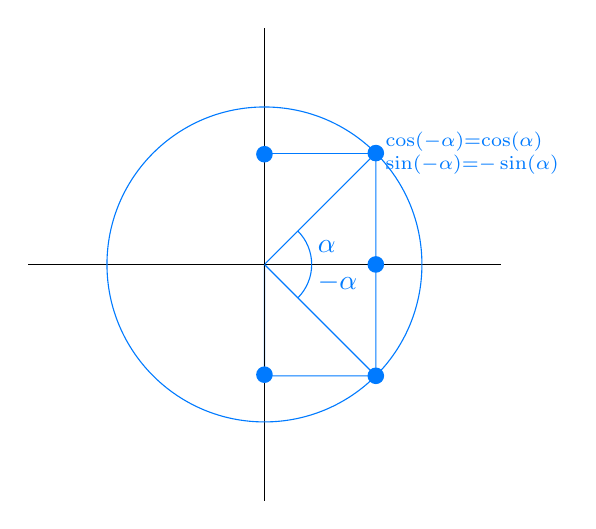
\begin{tikzpicture}[scale=2]
                  \draw[lightblue] (0,0) -- (45:1) node[right] {$\begin{subarray}{l}
                              \cos(-\alpha)=\cos(\alpha)\\
                              \sin(-\alpha)=-\sin(\alpha)
                        \end{subarray}$} -- (315:1) -| (0,0);
                  \draw[lightblue] (45:1) -| (0,0);
                  \draw (-1.5,0) -- (1.5,0);
                  \draw (0,-1.5) -- (0,1.5);
                  \draw[lightblue] (0,0) circle (1);
                  \draw[lightblue] (0,0) -- (315:1);
                  \fill[lightblue] (45:1) circle (1.5pt);
                  \fill[lightblue] (315:1) circle (1.5pt);
                  \fill[lightblue] ($(45:1)!0.5!(315:1)$) circle (1.5pt);
                  \fill[lightblue] (0,0.7) circle (1.5pt);
                  \fill[lightblue] (0,-0.7) circle (1.5pt);
                  \draw[lightblue] (0.3,0) arc (0:45:0.3) node[midway,right] {$\alpha$};
                  \draw[lightblue] (0.3,0) arc (0:-45:0.3) node[midway,right] {$-\alpha$};
            \end{tikzpicture}
      \end{center}
      
      $f(-x)=\left(\cos(-x)\right)^2=\left(\cos(x)\right)^2=f(x)$
      
      Como $f(-x)=f(x)$ entonces, podemos asegurar que $f(x)$ presenta \lb{simetría par}.
      \item $\db{f(x)=-\sin(x^3)}$
      
      $f(-x)=-\sin((-x)^3)=-\sin(-x^3)=-\left[-\sin(x^3)\right]=-f(x)$
      
      Por lo tanto, como $f(-x)=-f(x)$, diremos que $f(x)$ tiene \lb{simetría impar}
\end{enumerate}
\item \lb{Exprese en la forma $A\sin(x+c)$ la función $f(x)=\sin(x)+\sqrt{3}\cos(x)$. Observación: Puede utilizar números complejos para obtener la expresión.}

\begin{minipage}[l]{\textwidth}
      \begin{wrapfigure}{r}{0.5\textwidth}
            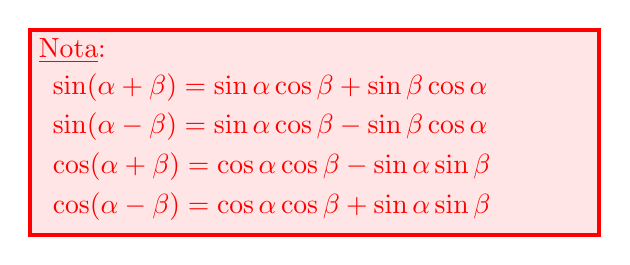
\begin{tikzpicture}[baseline=(current bounding box.center)]
                  \node[red,draw=red,fill=red!10,line width=1.5pt,text width=7cm] {\underline{Nota}:\\
                  $\begin{array}{l}
                        \sin(\alpha+\beta)=\sin\alpha\cos\beta+\sin\beta\cos\alpha\\
                        \sin(\alpha-\beta)=\sin\alpha\cos\beta-\sin\beta\cos\alpha\\
                        \cos(\alpha+\beta)=\cos\alpha\cos\beta-\sin\alpha\sin\beta\\
                        \cos(\alpha-\beta)=\cos\alpha\cos\beta+\sin\alpha\sin\beta
                  \end{array}$};
            \end{tikzpicture}
      \end{wrapfigure}
      
      
      $\begin{aligned}
            f(x)&=A\sin(x+c)\\
            &=A\left[\bboxed{\sin x}\cos c+\sin c\bboxed{\cos x}\right]\\
            &=\bboxed{\sin x}+\sqrt{3}\bboxed{\cos x}
      \end{aligned}$\\
      $\begin{array}{l}
                  \begin{cases}
                        A\cos c=1\\
                        A\sin c=\sqrt{3}
                  \end{cases}\\ \hline
                  \text{Dividido }\tan c=\sqrt{3}
            \end{array}\begin{array}{l}
            \longrightarrow A\cdot\dfrac{1}{2}=1\longrightarrow A=2\\
            \\
            \longrightarrow c=\dfrac{\pi}{3}
            \end{array}$\\
            $\bboxed{f(x)=2\sin\left(x+\dfrac{\pi}{3}\right)}$
\end{minipage}

\item \lb{Estudiar la continuidad y derivabilidad de las siguientes funciones:}

$\db{f(x)=\begin{cases}
            x^2 & x\ge1\\
            ax+b & x<1
\end{cases}}$

\underline{Continuidad:}
\begin{itemize}
      \item $\forall\,x<1\:f(x)$ es continua para ser un polinomio.
      \item $\forall\,x>1\:f(x)$ es continua para ser un polinomio.
\end{itemize}
Vamos la condición que debe verificarse para sea continua en $x=1$:

$\begin{rcases}
      \lim_{x\to1^-}(ax+b)=a+b\\
      \lim_{x\to1^+}x^2=1\\
      f(1)=1
\end{rcases}\bboxed{a+b=1}$ Condición que debe verificarse para que $f(x)$ sea continua en $x=1$.

\underline{Derivabilidad:}
\begin{itemize}
      \item $\forall\,x<1\:f(x)$ es derivable para ser un polinomio.\\
      \item $\forall\,x<1\:f(x)$ es derivable para ser un polinomio.
\end{itemize}
Veamos la condición que debe verificarse para sea derivable en $x=1$:

{\small$f'(1)=\lim_{x\to1}\dfrac{f(x)-f(1)}{x-1}=\left\{\begin{array}{l}
      \lim_{x\to1^-}\dfrac{ax+b-1}{x-1}=\{a+b=1\longrightarrow b-1=a\}=\lim_{x\to1}\dfrac{ax-a}{x-1}=\lim_{x\to1}\dfrac{\cancel{a(x+1)}}{\cancel{x-1}}=a\\
      \lim_{x\to1^+}\dfrac{x^2-1}{x-1}=\lim_{x\to1}\dfrac{\cancel{(x-1)(x+1)}}{\cancel{(x-1)}}=2
\end{array}\right\}$ }

Para que $f(x)$ sea derivable en $x=1$, debe verificarse que 

$\bboxed{\begin{array}{l}
            a=2\\
            b=-1
\end{array}}$ \lb{Condición para que sea continua y derivable en $x=1$.}

\item \lb{Calcular el desarrollo de Taylor hasta orden 5 de $f(x)=\sin(x)$ centrado en $a=0$.}

\begin{minipage}[l]{\textwidth}
      \begin{wrapfigure}[4]{r}{0.6\textwidth}
            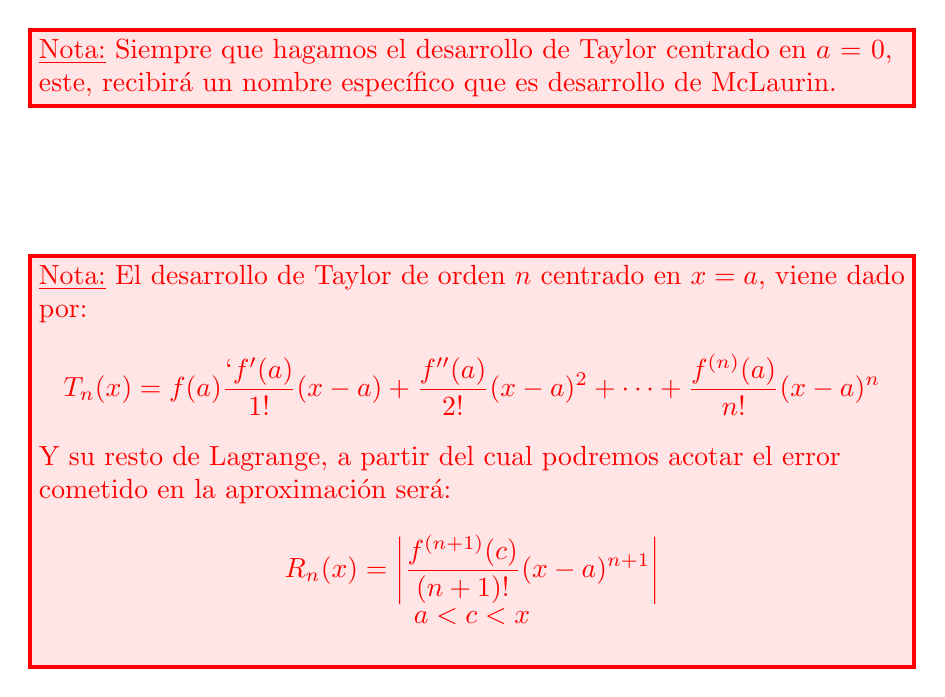
\begin{tikzpicture}[baseline=(current bounding box.center)]
                  \node[red,draw=red,fill=red!10,line width=1.5pt,text width=11cm] at (0,0) {\underline{Nota:} Siempre que hagamos el desarrollo de Taylor centrado en $a=0$, este, recibirá un nombre específico que es desarrollo de McLaurin.};
                  
                  \node[red,draw=red,fill=red!10,line width=1.5pt,text width=11cm] at (0,-5) {\underline{Nota:} El desarrollo de Taylor de orden $n$ centrado en $x=a$, viene dado por: \[ T_n(x)=f(a)\dfrac{`f'(a)}{1!}(x-a)+\dfrac{f''(a)}{2!}(x-a)^2+\cdots+\dfrac{f^{(n)}(a)}{n!}(x-a)^n \]Y su resto de Lagrange, a partir del cual podremos acotar el error cometido en la aproximación será: \[ \underset{\displaystyle a<c<x}{R_n(x)=\left|\dfrac{f^{(n+1)}(c)}{(n+1)!}(x-a)^{n+1}\right|} \]};
            \end{tikzpicture}
      \end{wrapfigure}
      
      Como queremos hallar el desarrollo de Taylor de orden 5 en $a=0$:
      
      $T_5(x)=\cancel{f(0)}+\dfrac{f'(0)}{1!}x+\cancel{\dfrac{f''(0)}{2!}x^2}+\dfrac{f'''(0)}{3!}x^3+\cancel{\dfrac{f^{\mathrm{iv}}(0)}{4!}x^4}+\dfrac{f^{\mathrm{v}}(0)}{5!}x^5$\\
      $\begin{array}{l}
            f(x)=\sin(x)\longrightarrow f(0)=0\\
            f'(x)=\cos(x)\longrightarrow f'(0)=1\\
            f''(x)-\sin(x)\longrightarrow f''(0)=0\\
            f'''(x)=-\cos(x)\longrightarrow f'''(0)=-1\\
            f^{\mathrm{iv}}(x)=\sin(x)\longrightarrow f^{\mathrm{iv}}(0)=0\\
            f^{\mathrm{v}}(x)=\cos(x)\longrightarrow f^{\mathrm{v}}(0)=1\\
            T_5(x)=x-\dfrac{1}{3!}x^3+\dfrac{1}{5!}x^5\\
            \\
            \bboxed{\sin(x)\simeq x-\dfrac{x^3}{6}+\dfrac{x^5}{120}+\mathrm{o}(x^6)}
      \end{array}$
      
      "o pequeña" y representa a todos los términos que no ponemos y tienen todos en común grado 6.
\end{minipage}

\item \lb{Obtener el desarrollo de McLaurin de orden 4 de la función $f(x)=e^{x}$}

Como queremos el desarrollo de McLaurin de orden 4, será en $a=0$.

$T_4(x)=f(0)+\dfrac{f'(0)}{1!}x+\dfrac{f''(0)}{2!}x^2+\dfrac{f'''(0)}{3!}x^3+\dfrac{f^{\mathrm{iv}}(0)}{4!}x^4$

$\begin{array}{l}
      f(x)=e^x\longrightarrow f(0)=1\\
      f'(x)=e^x\longrightarrow f'(0)=1\\
      f''(x)=e^x\longrightarrow f''(0)=1\\
      f'''(x)=e^x\longrightarrow f'''(0)=1\\
      f^{\mathrm{iv}}(x)=e^x\longrightarrow f^{\mathrm{iv}}(0)=1\\
\end{array}\qquad\begin{array}{l}
T_4(x)=1+\dfrac{1}{1!}x+\dfrac{1}{2!}x^2+\dfrac{1}{3!}x^3+\dfrac{1}{4!}x^4\\
\\
\bboxed{e^x=1+x+\dfrac{x^2}{2}+\dfrac{x^3}{6}+\dfrac{x^4}{24}+\mathrm{o}(x^5)}
\end{array}$

\pagebreak

\item \lb{Hallar el desarrollo de McLaurin de orden 4 de la función $f(x)=\ln(1+x)$}

Como queremos el desarrollo de McLaurin $(a=0)$, hasta orden 4, tendremos que:

$T_4(x)=f(0)+\dfrac{f'(0)}{1!}x+\dfrac{f''(0)}{2!}x^2+\dfrac{f'''(0)}{3!}x^3+\dfrac{f^{\mathrm{iv}}(0)}{4!}x^4$

$\begin{array}{l}
      f(x)=\ln(1+x)\longrightarrow f(0)=0\\
      f'(x)=\dfrac{1}{1+x}=(1+x)^{-1}\longrightarrow f'(0)=1\\
      f''(x)=(-1)(1+x)^{-2}=-\dfrac{1}{(1+x)^2}\longrightarrow f''(0)=-1\\
      f'''(x)=2(1+x)^{-3}=\dfrac{2}{(1+x)^3}\longrightarrow f'''(0)=2\\
      f^{\mathrm{iv}}(x)=-6(1+x)^{-4}=-\dfrac{6}{(1+x)^4}\longrightarrow f^{\mathrm{iv}}(0)=-6
\end{array}\qquad\begin{array}{l}
T_4(x)=\dfrac{1}{1!}x-\dfrac{1}{2!}x^2+\dfrac{2}{3}x^3-\dfrac{6}{4!}x^4\\
T_4(x)=x-\dfrac{x^2}{2}+\dfrac{x^3}{3}-\dfrac{x^4}{4}\\
\\
\bboxed{\ln(x+1)=x-\dfrac{x^2}{2}+\dfrac{x^3}{3}-\dfrac{x^4}{4}+\mathrm{o}(x^5)}
\end{array}$

\item \lb{Calcular el siguiente límite: \[ \lim_{x\to0}\dfrac{e^x-1-x-x^2}{x^2} \]}

\begin{minipage}[l]{\textwidth}
      \begin{wrapfigure}{r}{0.35\textwidth}
            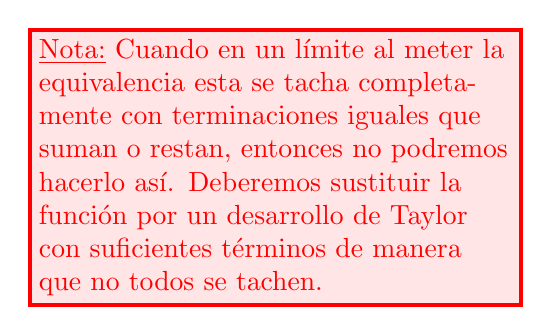
\begin{tikzpicture}[baseline=(current bounding box.center)]
                  \node[red,draw=red,fill=red!10,line width=1.5pt,text width=6cm] {\underline{Nota:} Cuando en un límite al meter la equivalencia esta se tacha completamente con terminaciones iguales que suman o restan, entonces no podremos hacerlo así. Deberemos sustituir la función por un desarrollo de Taylor con suficientes términos de manera que no todos se tachen.};
            \end{tikzpicture}
      \end{wrapfigure}
      
      $\lim_{x\to0}\dfrac{e^x-1-x-x^2}{x^2}=\left(\dfrac{0}{0}\right)=\left\{\begin{array}{l}
            \text{Equivalencia:}\\
            e^x\leadsto_0 1+x
      \end{array}\right\}=\overset{\rc{\mathrm{Error}}}{\fcolorbox{red}{red!10}{$\lim_{x\to0}\dfrac{\cancel{1}+\cancel{x}-\cancel{1}-\cancel{x}-x^2}{x^2}$}}$
      
      $\rboxed{\bboxed{e^x=1+x+\dfrac{x^2}{2}+\dfrac{x^3}{6}}+\dfrac{x^4}{24}+\mathrm{o}(x^5)}$
      
      $\lim_{x\to0}\dfrac{e^x-1-x-x^2}{x^2}=\lim_{x\to0}\dfrac{\cancel{1}+\cancel{x}+\frac{x^2}{2}+\frac{x^3}{6}+\mathrm{o}(x^4)-\cancel{1}-\cancel{x}-x^2}{x^2}=\lim_{x\to0}\dfrac{-\frac{1}{2}x^2+\frac{x^3}{6}+\mathrm{o}(x^4)}{x^2}=\lim_{x\to0}\dfrac{\cancel{x^2}\left[-\frac{1}{2}+\frac{x}{6}+\mathrm{o}(x^2)\right]}{\cancel{x^2}}=\lim_{x\to0}\left(-\dfrac{1}{2}+\tozero{\dfrac{x}{6}}+\tozero{\mathrm{o}(x^2)}\right)=\bboxed{-\dfrac{1}{2}}$
\end{minipage}
\item \lb{Hallar la suma de las series:}

$\db{\sum_{n=0}^{\infty}\dfrac{1}{2^{n+3}}=}\sum_{n=0}^{\infty}\dfrac{1}{2^n\cdot2^3}=\dfrac{1}{8}\sum_{n=0}^{\infty}\dfrac{1}{2^n}$

Para estudiar la convergencia, lo que haremos será aplicar el criterio de la raíz: \begin{center}
      $\lim_{n\to\infty}\sqrt[\cancel{n}]{\dfrac{1}{2^{\cancel{n}}}}=\dfrac{1}{2}<1$ La serie es convergente.
\end{center}
Para sumarla lo que haremos será darnos cuenta de que, al ser una exponencial, debemos sumarla. Como una serie geométrica: 

$\begin{array}{l}
      \sum_{n=0}^{\infty}\dfrac{1}{2^n}=\sum_{n=0}^{\infty}\left(\dfrac{1}{2}\right)^n=\sum_{n=0}^{\infty}b_n=\lim_{n\to\infty}\lbb{\sum_{j=0}^{n}b_j}{S_n}=\lim_{n\to\infty}\dfrac{b_0-b_{n+1}}{1-r}=\lim_{n\to\infty}\dfrac{1-\tozero{\left(\frac{1}{2}^{n+1}\right)}}{1-\frac{1}{2}}=\dfrac{1}{\frac{1}{2}}=2\\
      b_n=\left(\dfrac{1}{2}\right)^n\\
      r=\dfrac{b_2}{b_1}=\dfrac{1}{2}\\
      \begin{array}{l|l|l}
            S_n=b_0&\bcancel{+b_1+b_2+b_3+\cdots+b_n}& \\
            rS_n= & \bcancel{-b_1-b_2-b_3-\cdots-b_n}&-b_{n+1}\\ \hline
            \multicolumn{3}{l}{\text{\underline{Resto}}\longrightarrow(1-r)S_n=b_0-b_{n+1}\longrightarrow S_n=\dfrac{b_0-b_{n+1}}{1-r}}
      \end{array}\\
      \sum_{n=0}^{\infty}\dfrac{1}{2^{n+3}}=\sum_{n=0}^{\infty}\dfrac{1}{2^n\cdot2^3}=\dfrac{1}{8}\sum_{n=0}^{\infty}\dfrac{1}{2^n}=\dfrac{1}{8}\cdot2=\dfrac{1}{4}\longrightarrow\bboxed{\sum_{n=0}^{\infty}\dfrac{1}{2^{n+3}}=\dfrac{1}{4}}
\end{array}$
\item \lb{Hallar la suma de las series:}

$\db{\sum_{n=0}^{\infty}\dfrac{2^{n+3}}{3^3}=}\sum_{n=0}^{\infty}\dfrac{2^n\cdot2^3}{3^3}=\dfrac{8}{27}\cdot\sum_{n=0}^{\infty}2^n$

Pero como $\lim_{n\to\infty}2^n=+\infty\neq0\longrightarrow$ entonces no verifica la condición necesaria que deben verificar las series de términos no negativos, y es que $\lim_{n\to\infty}a_n=0$.

Por lo tanto, como no verifica la condición necesaria, entonces no es convergente, es decir, la serie es divergente y su suma sería $+\infty$.
\item \lb{Determine de las siguientes sucesiones $(a_n)_n$ cuáles son convergentes y calcule el límite en dicho caso.}

$\db{a_n=\log(n)-\log(n+1)}$

$\begin{array}{l}
      \lim_{n\to\infty}\left[\log(n)-\log(n+1)\right]=(\infty-\infty)=\lim_{n\to\infty}\log\left(\dfrac{n}{n+1}\right)=\lb{(\ast)}=\log(1)=\bboxed{0}\\
      \lim_{n\to\infty}\dfrac{n}{n+1}=\left(\dfrac{\infty}{\infty}\right)=\lim_{n\to\infty}\dfrac{\frac{n}{n}}{\frac{n}{n}+\tozero{\frac{1}{n}}}=1
\end{array}$
\item \lb{Determine de las siguientes sucesiones $(a_n)_n$ cuáles son convergentes y calcule el límite en dicho caso.}

\begin{minipage}[l]{\textwidth}
      \begin{wrapfigure}{r}{0.35\textwidth}
            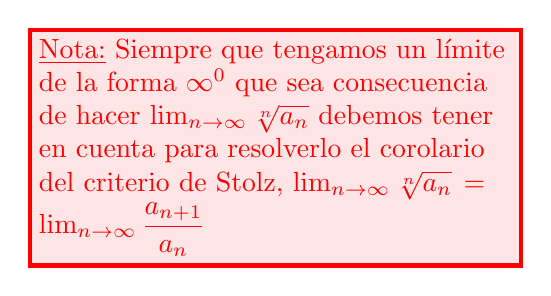
\begin{tikzpicture}[baseline=(current bounding box.center)]
                  \node[red,draw=red,fill=red!10,line width=1.5pt,text width=6cm] {\underline{Nota:} Siempre que tengamos un límite de la forma $\infty^0$ que sea consecuencia de hacer $\lim_{n\to\infty}\sqrt[n]{a_n}$ debemos tener en cuenta para resolverlo el corolario del criterio de Stolz, $\lim_{n\to\infty}\sqrt[n]{a_n}=\lim_{n\to\infty}\dfrac{a_{n+1}}{a_n}$};
            \end{tikzpicture}
      \end{wrapfigure}

$\db{a_n=\sqrt[n]{n^2}}$

$\lim_{n\to\infty}\sqrt[n]{n^2}=(\infty^0)=\left\{\lim_{n\to\infty}\overset{a_n=n^2}{\sqrt[n]{a_n}}=\lim_{n\to\infty}\dfrac{a_{n+1}}{a_n}\right\}=\lim_{n\to\infty}\dfrac{a_{n+1}}{a_n}=\lim_{n\to\infty}\dfrac{(n-1)^2}{n^2}=\lim_{n\to\infty}\dfrac{n^2+2n+1}{n^2}=\lim_{n\to\infty}\left(\dfrac{n^2}{n^2}+\tozero{\dfrac{2n}{n^2}}+\tozero{\dfrac{1}{n^2}}\right)=\bboxed{1}$
\end{minipage}
\pagebreak
\item \lb{Calcule $\lim_{x\to\frac{\pi}{2}}\dfrac{\cos(x)}{x-\frac{\pi}{2}}$ utilizando la definición de derivada}

\begin{minipage}[l]{\textwidth}
      \begin{wrapfigure}{r}{0.35\textwidth}
            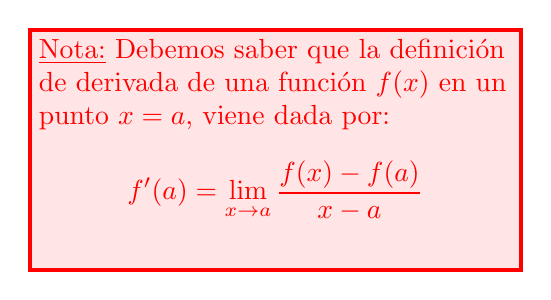
\begin{tikzpicture}[baseline=(current bounding box.center)]
                  \node[red,draw=red,fill=red!10,line width=1.5pt,text width=6cm] {\underline{Nota:} Debemos saber que la definición de derivada de una función $f(x)$ en un punto $x=a$, viene dada por: \[ f'(a)=\lim_{x\to a}\dfrac{f(x)-f(a)}{x-a} \]};
            \end{tikzpicture}
      \end{wrapfigure}
      
      $\lim_{x\to\frac{\pi}{2}}\dfrac{\cos(x)}{x-\frac{\pi}{2}}=\lim_{x\to\frac{\pi}{2}}\dfrac{\cos(x)-\cos\left(\frac{\pi}{2}\right)}{x-\frac{\pi}{2}}=\lim_{x\to\frac{\pi}{2}}\dfrac{f(x)-f\left(\frac{\pi}{2}\right)}{x-\frac{\pi}{2}}=f'\left(\dfrac{\pi}{2}\right)$
      
      Como $f(x)=\cos(x)\longrightarrow f'(x)=-\sin(x)\longrightarrow f'\left(\dfrac{\pi}{2}\right)=-1$ 
      
      Por lo tanto: \[ \bboxed{\lim_{x\to\frac{\pi}{2}}\dfrac{\cos(x)}{x-\frac{\pi}{2}}=-1 }\]
\end{minipage}

\vspace{2cm}

\item \lb{Calcular los siguiente límites:}

\begin{minipage}[l]{\textwidth}
      \begin{wrapfigure}{r}{0.45\textwidth}
            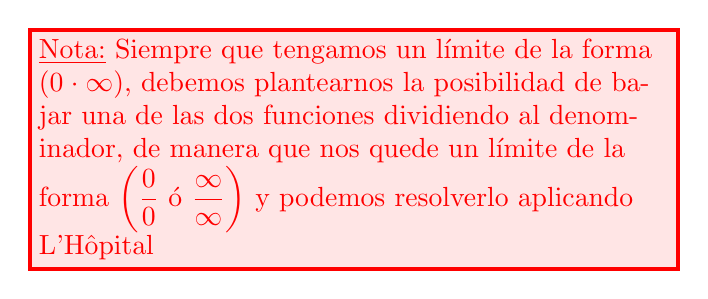
\begin{tikzpicture}[baseline=(current bounding box.center)]
                  \node[red,draw=red,fill=red!10,line width=1.5pt,text width=8cm] {\underline{Nota:} Siempre que tengamos un límite de la forma $(0\cdot\infty)$, debemos plantearnos la posibilidad de bajar una de las dos funciones dividiendo al denominador, de manera que nos quede un límite de la forma $\left(\dfrac{0}{0}\text{ ó }\dfrac{\infty}{\infty}\right)$ y podemos resolverlo aplicando L'Hôpital};
            \end{tikzpicture}
      \end{wrapfigure}
      
      $\db{\lim_{x\to\frac{1}{2}}(2x^2-3x+1)\tan(\pi x)=}(0\cdot\infty)=\lim_{x\to\frac{1}{2}}\dfrac{2x^2-3x+1}{\cot(\pi x)}=\left(\dfrac{0}{0}\right)=\{\text{L'Hôpital}\}=\lim_{x\to\frac{1}{2}}\dfrac{4x-2}{\frac{-1}{\sin^2(\pi x)}\cdot\pi}=\lim_{x\to\frac{1}{2}}-\dfrac{(4x-3)\sin^2(\pi x)}{\pi}=\dfrac{1}{\pi}$
\end{minipage}

\vspace{1cm}

\item \lb{Calcular el siguiente límite: \[ \lim_{x\to1}\dfrac{(x-1)(1-\cos(x-1))}{\sin(x-1)\cdot\arctan^2(x-1)} \]}

$\lim_{x\to1}\dfrac{(x-1)(1-\cos(x-1))}{\sin(x-1)\cdot\arctan^2(x-1)}=\left(\dfrac{0}{0}\right)=\lim_{x\to1}\dfrac{\cancel{(x-1)}\cdot\frac{\cancel{(x-1)^2}}{2}}{\cancel{(x-1)}\cdot\cancel{(x-1)^2}}=\bboxed{\dfrac{1}{2}}$

Vamos a aplicar equivalencias:

$\begin{array}{l}
      \sin(x)\leadsto_0x\longrightarrow\sin(x-1)\leadsto_1(x-1)\\
      \arctan(x)\leadsto_0x\longrightarrow\arctan(x-1)\leadsto_1(x-1)\\
      \cos(x)\leadsto_01-\dfrac{x^2}{2}\longrightarrow1-\cos(x)\leadsto_0\dfrac{x^2}{2}\longrightarrow1-\cos(x-1)\leadsto_1\dfrac{(x-1)^2}{2}
\end{array}$

\item \lb{Hallar $a$ y $b$ para que este límite sea un número real: \[ L=\lim_{x\to0}\dfrac{x+a\sin(x)+b\tan(x)}{x^5} \]}

            
\begin{tikzpicture}[baseline=(current bounding box.center)]
                  \node[red,draw=red,fill=red!10,line width=1.5pt, text width=17.5cm] {\underline{Nota:} Para que este límite sea un número real, debe cumplirse que los términos del numerador terminen teniendo grado 5, para que se compense el denominador y salga una constante.};
            \end{tikzpicture}
      
      Lo que vamos a hacer es transformar $\sin(x)$ y $\tan(x)$ en polinomios mediante desarrollos de Taylor:
      
      $\begin{array}{l}
            f(x)=\sin(x)\longrightarrow f(0)=0\\
            f'(x)=\cos(x)\longrightarrow f'(0)=1\\
            f''(x)=-\sin(x)\longrightarrow f''(0)=0\\
            f'''(x)=-\cos(x)\longrightarrow f'''(0)=-1\\
            f^{\mathrm{iv}}(x)=\sin(x)\longrightarrow f^{\mathrm{iv}}(0)=0\\
            f^{\mathrm{v}}(x)=\cos(x)\longrightarrow f^{\mathrm{v}}(0)=1\\
      \end{array}\qquad\bboxed{\sin(x)=x-\dfrac{1}{3!}x^3+\dfrac{1}{5!}x^5+\mathrm{o}(x^6)}$
      
      \vspace{1cm}
      
      $\begin{array}{l}
            f(x)=\tan(x)\longrightarrow f(0)=0\\
            f'(x)=\dfrac{1}{\cos^2(x)}\longrightarrow f'(0)=1\\
            f''(x)=\dfrac{-2\cos(x)\cdot(-\sin(x))}{\cos^4(x)}=\dfrac{2\sin(x)}{\cos^3(x)}\longrightarrow f''(0)=0\\
            \begin{aligned}
                  f'''(x)&=\dfrac{2\cos(x)\cdot\cos^{\cancel{3}}(x)-3\cancel{\cos^2(x)}\cdot(-\sin(x))\cdot2\sin(x)}{\cos^{\cancel{6}\lb{4}}(x)}=\dfrac{2\cos^2(x)+6\sin^2(x)}{\cos^4(x)}\\
                  &=\dfrac{2+4\sin^2(x)}{\cos^4(x)}\longrightarrow f'''(0)=2
            \end{aligned}\\
            \begin{aligned}
                  f^{\mathrm{iv}}(x)&=\dfrac{8\sin(x)\cos(x)\cos^{\cancel{4}}(x)-(2+4\sin^2(x))\cdot4\cancel{\cos^3(x)}(-\sin(x))}{\cos^{\cancel{8}\lb{5}}(x)}\\
                  &=\dfrac{8\sin(x)\cos^2(x)+8\sin(x)+16\sin^3(x)}{\cos^5(x)}\longrightarrow f^{\mathrm{iv}}(0)=0
            \end{aligned}\\
            f^{\mathrm{v}}(x)=\dfrac{(16\cos(x)+14\sin^2(x)\cos(x))-(16\sin(x)+8\sin^3(x))5\cos^4(x)(-\sin(x))}{\cos^{10}(x)}\longrightarrow f^{\mathrm{v}}(0)=16\\
            \tan(x)=\dfrac{1}{1!}x+\dfrac{2}{3!}x^3+\dfrac{16}{5!}x^5+\mathrm{o}(x^6)\\
            \\
            
            \bboxed{\tan(x)=x+\dfrac{1}{3}x^3+\dfrac{2}{15}x^5+\mathrm{o}(x^6)}\\
            \\
            \begin{aligned}
                  L&=\lim_{x\to0}\dfrac{x+a\sin(x)+b\tan(x)}{x^5}=\lim_{x\to0}\dfrac{x+a\left(x-\frac{1}{6}x^3+\frac{1}{120}x^5+\mathrm{o}(x^6)\right)+b\left(x+\frac{1}{3}x^3+\frac{2}{15}+\mathrm{o}(x^6)\right)}{x^5}\\
                  &=\lim_{x\to0}\dfrac{(1+a+b)x+\left(-\frac{a}{6}+\frac{b}{3}\right)x^3+\left(\frac{a}{120}+\frac{2b}{15}\right)x^5+\mathrm{o}(x^6)}{x^5}\\
                  &=\left\{\begin{array}{ll}
                        1+a+b=0\longrightarrow 1+3b=0 & \longrightarrow\\
                        -\dfrac{a}{6}+\dfrac{b}{3}=0\longrightarrow a=2b & \longrightarrow
                  \end{array}\bboxed{\begin{array}{l}
                        b=-\dfrac{1}{3}\\
                        a=-\dfrac{2}{3}
                        \end{array}}\right\}=\lim_{x\to0}\dfrac{\left(-\frac{1}{180}-\frac{2}{45}\right)x^5+\mathrm{o}(x^6)}{x^5}\\
                  &=\lim_{x\to0}\dfrac{\cancel{x^5}\left[-\frac{9}{180}+\tozero{\mathrm{o}(x)}\right]}{\cancel{x^5}}=\bboxed{-\dfrac{1}{20}}
            \end{aligned}
      \end{array}$
\item \lb{Estudie los límites laterales:}

\begin{enumerate}[label=\color{red}\alph*)]
      \item \db{$f(x)=\dfrac{|x|}{x^2+x}$ en $x=0$.}
      
      $|x|=\begin{cases}
            -x & \text{si }x<0\\
            x & \text{si }x>0
      \end{cases}\quad\begin{array}{l}
      \lim_{x\to0^-}\dfrac{|x|}{x^2+x}=\lim_{x\to0^-}\dfrac{-\cancel{x}}{\cancel{x}(x+1)}=\lim_{x\to0^-}\dfrac{-1}{x+1}=-1\\
      \lim_{x\to0^+}\dfrac{|x|}{x^2+x}=\lim_{x\to0^+}\dfrac{x}{x(x+1)}=\lim_{x\to0^+}\dfrac{1}{x+1}=1
      \end{array}\nexists\lim_{x\to0}\dfrac{|x|}{x^2+x}$
      
      En $x=0$ esta función presenta una discontinuidad inevitable de salto finito.
      \item \db{$f(x)=e^{\frac{|x|}{x}}$ en $x=0$.}
      
      $\begin{array}{l}
            \lim_{x\to0^-}e^{\frac{|x|}{x}}=\lim_{x\to0^-}e^{-\frac{x}{x}}=e^{-1}\\
            \lim_{x\to0^+}e^{\frac{|x|}{x}}=\lim_{x\to0^+}e^{\frac{x}{x}}=e^{1}
      \end{array}\nexists\lim_{x\to0}e^{\frac{|x|}{x}}$
      \item \db{$f(x)=\dfrac{1+e^{\frac{1}{x}}}{1-e^{\frac{1}{x}}}$ en $x=0$.}
      
      $\begin{array}{l}
            \lim_{x\to0^-}\dfrac{1+e^{\frac{1}{x}}}{1-e^{\frac{1}{x}}}=\dfrac{1+e^{-\infty}}{1-e^{-\infty}}=\left\{e^{-\infty}=\dfrac{1}{e^{\infty}}=\dfrac{1}{+\infty}=0\right\}=1\\
            \lim_{x\to0^+}\dfrac{1+e^{\frac{1}{x}}}{1-e^{\frac{1}{x}}}=\dfrac{1+e^{+\infty}}{1-e^{+\infty}}=\left(\dfrac{\infty}{\infty}\right)=\lim_{x\to0^+}\dfrac{\frac{1}{e^{\frac{1}{x}}}+\frac{e^{\frac{1}{x}}}{e^{\frac{1}{x}}}}{\frac{1}{e^{\frac{1}{x}}}-\frac{e^{\frac{1}{x}}}{e^{\frac{1}{x}}}}=\dfrac{\tozero{\frac{1}{\infty}}+1}{\tozero{\frac{1}{\infty}}-1}=-1
      \end{array}\quad\nexists\lim_{x\to0}\dfrac{1+e^{\frac{1}{x}}}{1-e^{\frac{1}{x}}}$
\end{enumerate}
\item \lb{Hallar el desarrollo de McLaurin hasta orden 5 de la función $f(x)=\sin(x)$. Utilizarlo para dar una aproximación de $\sin(0.2)$ y dar una cota de error.}

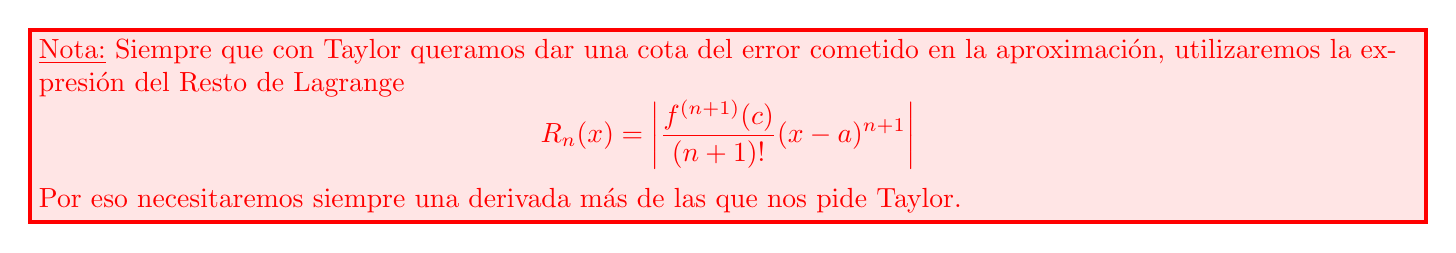
\begin{tikzpicture}
      \node[red,draw=red,fill=red!10,rectangle, line width=1.5,text width=17.5cm]  {\underline{Nota:} Siempre que con Taylor queramos dar una cota del error cometido en la aproximación, utilizaremos la expresión del Resto de Lagrange \[ R_n(x)=\left|\dfrac{f^{(n+1)}(c)}{(n+1)!}(x-a)^{n+1}\right| \]Por eso necesitaremos siempre una derivada más de las que nos pide Taylor.};
\end{tikzpicture}

Como queremos el desarrollo de McLaurin (Taylor con $a=0$) hasta orden 5: \[ T_5(x)=f(0)+\dfrac{f'(0)}{1!}x+\dfrac{f''(0)}{2!}x^2+\dfrac{f'''(0)}{3!}x^3+\dfrac{f^{\mathrm{iv}}(0)}{4!}x^4+\dfrac{f^{\mathrm{v}}(0)}{5!}x^5 \]

$\begin{array}{l}
      f(x)=\sin(x)\longrightarrow f(0)=0\\
      f'(x)=\cos(x)\longrightarrow f'(0)=1\\
      f''(x)=-\sin(x)\longrightarrow f''(0)=0\\
      f'''(x)=-\cos(x)\longrightarrow f'''(0)=-1\\
      f^{\mathrm{iv}}(x)=\sin(x)\longrightarrow f^{\mathrm{iv}}(0)=0\\
      f^{\mathrm{v}}(x)=\cos(x)\longrightarrow f^{\mathrm{v}}(0)=1\\
\end{array}\quad\begin{array}{l}
T_5(x)=\dfrac{1}{1!}x-\dfrac{1}{3!}x^3+\dfrac{1}{5!}x^5\\
\\
\bboxed{T_5(x)=x-\dfrac{x^3}{6}+\dfrac{x^5}{120}}\\
\\
\bboxed{\sin(x)=x-\dfrac{x^3}{6}+\dfrac{x^5}{120}+\mathrm{o}(x^6)}
\end{array}$

Como queremos $\sin(0.2)\longrightarrow\bboxed{x=0.2}$

$\sin(0.2)\simeq0.2-\dfrac{0.2^3}{6}+\dfrac{0.2^5}{120}=0.19866933\longrightarrow\bboxed{\sin(0.2)\simeq0.19866933}$

Para encontrar la cota del error cometido en la aproximación: \[ R_5(x)=\underset{a<c<x}{\left|\dfrac{f^{\mathrm{vi}}(c)}{6!}\right|}=\underset{0<c<0.2}{\left|-\dfrac{\sin(c)}{720}(0.2)^6\right|}\underset{\begin{subarray}{c}
            \downarrow\\
            |\sin(c)|\le1
\end{subarray}}{\le}\dfrac{1}{720}(0.2)^6=88.88\cdot10^{-9} \]

\fcolorbox{lightblue}{lightblue!10}{El error cometido es $E<88.88\cdot10^{-9}$}

\item \lb{Sabiendo que $\dfrac{\pi}{4}=\arctan\left(\dfrac{1}{2}\right)+\arctan\left(\dfrac{1}{3}\right)$. Calcular el desarrollo de Taylor de orden 3 de la función $f(x)=\arctan(x)$ centrado en $a=0$. Utilizarlo para encontrar una aproximación de $\dfrac{\pi}{4}$. Dar una estimación del error.}

Sea $f(x)=\arctan(x)$. Queremos hallar: \[ T_3(x)=f(0)+\dfrac{f'(0)}{1!}x+\dfrac{f''(0)}{2!}x^2+\dfrac{f'''(0)}{3!}x^3 \] $\begin{array}{l}
      f(x)=\arctan(x)\longrightarrow f(0)=0\\
      f'(x)=\dfrac{1}{1+x^2}\longrightarrow f'(0)=1\\
      f''(x)=\dfrac{-2x}{(1+x^2)^2}\longrightarrow f''(0)=0\\
      f'''(x)=\dfrac{-2(1+x^2)^{\cancel{2}}+2x\cdot\cancel{(1+x^2)}\cdot2x}{(1+x^2)^{\cancel{4}3}}=\dfrac{-2+6x^2}{(1+x^2)^{3}}\longrightarrow f'''(0)=-2\\
      f^{\mathrm{iv}}(x)=\dfrac{12x(1+x^2)^{\cancel{3}}-(-2+6x^2)\cdot3(1+x^{\cancel{2}})^{\cancel{2}}\cdot2x}{(1+x^2)^{\cancel{6}\lb{4}}}=\dfrac{12x+\cancel{12x^3}+12x-36x^3}{(1+x^2)^{4}}=\dfrac{24x-24x^3}{(1+x^2)^{4}}
\end{array}$

Sustituyendo tenemos que: \[ \begin{array}{l}
      \bboxed{T_3(x)=x-\dfrac{1}{3}x^3}\longrightarrow\arctan(x)=x-\dfrac{1}{3}x^3+\mathrm{o}(x^4)\\
      R_3(x)=\underset{a<c<x}{\left|\dfrac{f^{\mathrm{iv}}(c)}{4!}(x-a)^4\right|}=\left|\dfrac{\frac{24c-24c^3}{(1+c^2)^4}}{24}(x)^4\right|=\underset{0<c<x}{\left|\dfrac{c-c^3}{(1+c^2)^4}x^4\right|}
\end{array} \]

Comenzamos con $\arctan\left(\dfrac{1}{2}\right)\longrightarrow x=\dfrac{1}{2}$


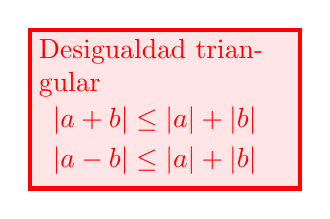
\begin{tikzpicture}[baseline=(current bounding box.center)]
         \node[red,draw=red,fill=red!10,line width=1.5pt,text width=3.2cm] {Desigualdad triangular\\
         $\begin{array}{l}
               |a+b|\le|a|+|b|\\
               |a-b|\le|a|+|b|
         \end{array}$};
\end{tikzpicture}$\begin{array}{l}
\arctan\left(\dfrac{1}{2}\right)\simeq\dfrac{1}{2}-\dfrac{1}{3}\left(\dfrac{1}{2}\right)^3=\dfrac{1}{2}-\dfrac{1}{24}=\dfrac{11}{24}=0.458333\longrightarrow\bboxed{\arctan\left(\dfrac{1}{2}\right)\simeq0.458333}\\
E_1=\underset{0<c<\frac{1}{2}}{\left|\dfrac{c-c^3}{(1+c^2)^4}\left(\dfrac{1}{2}\right)^4\right|}=\dfrac{|c-c^3|}{(1+c^2)^4}\left(\dfrac{1}{2}\right)^4<\dfrac{\frac{5}{8}}{1}\left(\dfrac{1}{2}\right)^4=0.0390625\\
|c-c^3|\le|c|+|c|^3<\dfrac{1}{2}+\left(\dfrac{1}{2}\right)^3=\dfrac{5}{8}
\end{array}$

Calculamos ahora: $\arctan\left(\dfrac{1}{3}\right)\longrightarrow x=\dfrac{1}{3}$

\[\begin{array}{l}
      \arctan\left(\dfrac{1}{3}\right)=\dfrac{1}{3}-\dfrac{1}{3}\left(\dfrac{1}{3}\right)^3+\mathrm{o}(x^4)\longrightarrow\bboxed{\arctan\left(\dfrac{1}{3}\right)\simeq0.320987}\\
      E_2=\underset{0<c<\frac{1}{3}}{\left|\dfrac{c-c^3}{(1+c^2)^4}\left(\dfrac{1}{3}^4\right)\right|}=\dfrac{|c-c^3|}{(1+c^2)^4}\left(\dfrac{1}{3}\right)^4<\dfrac{0.37037}{1}\left(\dfrac{1}{3}\right)^4=0.00457247\\
      |c-c^3|\le|c|+|c|^3<\dfrac{1}{3}+\left(\dfrac{1}{3}\right)^3=0.37037
\end{array}\] Por lo tanto tenemos que: $\dfrac{\pi}{4}=\arctan\left(\dfrac{1}{2}\right)+\arctan\left(\dfrac{1}{3}\right)\simeq0.458333+0.320987=0.77932$ \[ \bboxed{\begin{array}{c}
      \dfrac{\pi}{4}\simeq0.77932\\
      \mathrm{Error}<E_1+E_2=0.0390625+0.00457247=0.04363497
      \end{array}} \]
\item \lb{Obtener el desarrollo de McLaurin de orden 3 de la función $f(x)=\ln(1+x)$ y utilizarlo para dar un valor aproximado de $\ln(1.2)$. Dar una cota del error cometido en la aproximación.}

\[ T_3(x)=f(0)+\dfrac{f'(0)}{1!}x+\dfrac{f''(0)}{2!}x^2+\dfrac{f'''(0)}{3!}x^3 \]
$\begin{array}{l}
      f(x)=\ln(x)\longrightarrow f(0)=0\\
      f'(x)=\dfrac{1}{x+1}=(1+x)^{-1}\longrightarrow f'(0)=1\\
      f''(x)=(-1)(1+x)^{-2}=\dfrac{-1}{(1+x)^2}\longrightarrow f''(0)=-1\\
      f'''(x)=2(1+x)^{-3}=\dfrac{2}{(1+x)^3}\longrightarrow f'''(0)=2\\
      f^{\mathrm{iv}}(x)=-6(1+x)^{-4}=\dfrac{-6}{(1+x)^4}
\end{array}\qquad\begin{array}{l}
T_3(x)=x-\dfrac{1}{2!}x^2+\dfrac{2}{3!}x^3=x-\dfrac{1}{2}x^2+\dfrac{1}{3}x^3\\
\\
\bboxed{\log(1+x)=x-\dfrac{1}{2}x^2+\dfrac{1}{3}x^3+\mathrm{o}(x^4)}
\end{array}$

Como queremos $\log(1.2)=\log(1+x)\longrightarrow 1+x=1.2\longrightarrow\bboxed{x=0.2}$

$\begin{array}{l}
      \log(1.2)=0.2-\dfrac{1}{2}(0.2)^2+\dfrac{1}{3}(0.2)^3+\mathrm{o}(x^4)\\
      \\
      \bboxed{\log(1.2)\simeq0.182667}
\end{array}$

\underline{Acotación del resto:}
\[ \begin{array}{l}
      R_3(x)=\underset{a<c<x}{\left|\dfrac{f^{\mathrm{iv}}(c)}{4!}(x-a)^4\right|}=\left|\dfrac{\frac{-6}{(1+c)^4}}{24}(0.2^4)\right|=\underset{0<c<0.2}{\dfrac{1}{4(1+c)^4}(0.2)^4}<\dfrac{1}{4}(0.2)^4=0.0004\\
      \\
      \bboxed{E<0.0004}\lb{\text{ Cota de error}}
\end{array} \]
\item \lb{Calcule el siguiente límite sin utilizar L'Hôpital: \[ \lim_{x\to1}\dfrac{2x-2}{\sqrt[3]{26+x}-3}. \]}

$\begin{array}{l}
      \lim_{x\to1}\dfrac{2x-2}{\sqrt[3]{26+x}-3}=\left(\dfrac{0}{0}\right)=\lim_{x\to1}\dfrac{2\cancel{(x-1)}}{\frac{\cancel{(x-1)}}{\sqrt[3]{26+x)^2}+3\sqrt[3]{26+x}+9}}=\lim_{x\to1}2\left[\sqrt[3]{(26+x)^2}+3\sqrt[3]{26+x}+9\right]=\bboxed{54}\\
      \sqrt[3]{26+x}-3=b-a=\dfrac{b^3-a^3}{b^2+ba+a^2}=\dfrac{26+x-27}{\sqrt[3]{(26+x)^2}+3\sqrt[3]{26+x}+9}=\dfrac{x-1}{\sqrt[3]{26+x)^2}+3\sqrt[3]{26+x}+9}\\
      b^3-a^3=(b-a)(b^2+ba+a^2)
\end{array}$
\item \lb{Calcula el límite \[ \lim_{x\to0}\dfrac{(\sin(x)-x)^2}{(\log(1+x)-x)^3} \]}

\begin{minipage}[l]{\textwidth}


$\begin{array}{l}
      f(x)=\sin(x)\longrightarrow f(0)=0\\
      f'(x)=\cos(x)\longrightarrow f'(0)=1\\
      f''(x)=-\sin(x)\longrightarrow f''(0)=0\\
      f'''(x)=-\cos(x)\longrightarrow f'''(0)=-1\\
      f^{\mathrm{iv}}(x)=\sin(x)\longrightarrow f^{\mathrm{iv}}(0)=0\\
      f^{\mathrm{v}}(x)=\cos(x)\longrightarrow f^{\mathrm{v}}(0)=1\\
      \end{array}\qquad$
      
\begin{tikzpicture}[baseline=(current bounding box.center)]
      \node[red,draw=red,fill=red!10,line width=1.5pt,text width=10cm] {\underline{Nota:} Si al resolver un límite, metemos equivalencias, para estas al sustituir se anulan automáticamente, es porque no ha sido suficiente la información que necesitamos. Entonces lo que haremos en este caso será obtener mediante Taylor centrado en el punto del límite, un desarrollo de al menos 3 o 4 términos. Esto lo llamaremos desarrollos limitados.};
      \end{tikzpicture}
\end{minipage}

$ \begin{array}{l}
      T_5(x)=\cancel{f(0)}+\dfrac{f'(0)}{1!}x+\cancel{\dfrac{f''(0)}{2!}x^2}+\dfrac{f'''(0)}{3!}x^3+\cancel{\dfrac{f^{\mathrm{iv}}(0)}{4!}x^4}+\dfrac{f^{\mathrm{v}}(0)}{5!}x^5\\
      \\
      \bboxed{\sin(x)=x-\dfrac{1}{6}x^3+\dfrac{1}{120}x^5+\mathrm{o}(x^6)}\\
\end{array}$

\lb{Representa el grado menor de los términos que no poseemos}

$\begin{array}{l}
      g(x)=\log(1+x)\longrightarrow g(0)=0\\
      g'(x)=\dfrac{1}{x+1}=(1+x)^{-1}\longrightarrow g'(0)=1\\
      g''(x)=(-1)(1+x)^{-2}=-\dfrac{1}{(1+x)^2}\longrightarrow g''(0)=-1\\
      g'''(x)=2(1+x)^{-3}=\dfrac{2}{(1+x)^3}\longrightarrow g'''(0)=2
\end{array}\qquad\begin{array}{l}
T_3(x)=\cancel{g(0)}+\dfrac{f'(0)}{1!}x+\dfrac{g''(0)}{2!}x^2+\dfrac{g'''(0)}{3!}x^3\\
\\
\bboxed{\log(1+x)=x-\dfrac{1}{2}x^2+\dfrac{1}{3}x^3+\mathrm{o}(x^4)}
\end{array}$

$\begin{aligned}
      \lim_{x\to0}\dfrac{(\sin(x)-x)^2}{(\log(1+x)-x)^3}&=\lim_{x\to0}\dfrac{\left(\cancel{x}-\frac{1}{6}x^3+\frac{1}{120}x^5+\mathrm{o}(x^4)-\cancel{x}\right)^2}{\left(\cancel{x}-\frac{1}{2}x^2+\frac{1}{3}x^3+\mathrm{o}(x^4)-\cancel{x}\right)^3}=\lim_{x\to0}\dfrac{\left(-\frac{1}{6}x^3+\frac{1}{120}x^5+\mathrm{o}(x^4)\right)^2}{\left(-\frac{1}{2}x^2+\frac{1}{3}x^3+\mathrm{o}(x^4)\right)^3}\\
      &=\lim_{x\to0}\dfrac{\left[x^3\left(-\frac{1}{6}+\frac{1}{120}x^2+\mathrm{o}(x^3)\right)\right]^2}{\left[x^2\left(-\frac{1}{2}+\frac{1}{3}x+\mathrm{o}(x^2)\right)\right]^3}=\lim_{x\to0}\dfrac{\cancel{x^6}\left(-\frac{1}{6}+\tozero{\frac{1}{120}x^2}+\tozero{\mathrm{o}(x^3)}\right)^2}{\cancel{x^6}\left(-\frac{1}{2}+\tozero{\frac{1}{3}x}+\tozero{\mathrm{o}(x^2)}\right)^3}\\
      &=\dfrac{\frac{1}{36}}{-\frac{1}{8}}=-\dfrac{8}{36}=\bboxed{-\dfrac{2}{9}}
\end{aligned}$
\item \lb{Hallar $\mathbf{a,b,c}$ y $\mathbf{d}$ para que se cumpla \[ \lim_{x\to0}\dfrac{\log(1+x^2)-a-bx-cx^2-dx^3}{x^3}=0. \]}

En este límite vamos a calcular el desarrollo limitado de $\log(1+x^2)$ y lo vamos a sustituir: Para hallar el desarrollo de $\log(1+x^2)$, vamos a obtener el de $\log(1+x)$ y luego sustituiremos todas las $x$ por $x^2$

$\begin{array}{l}
      g(x)=\log(1+x)\longrightarrow g(0)=0\\
      g¡(x)=\dfrac{1}{1+x}=(1+x)^{-1}\longrightarrow g'(0)=1\\
      g''(x)=(-1)(1+x)^{-2}=-\dfrac{1}{(1+x)^2}\longrightarrow g''(0)=-1\\
      g'''(x)=2(1+x)^{-3}=\dfrac{2}{(1+x)^3}\longrightarrow g'''(0)=2
\end{array}\qquad\begin{array}{l}
T_3(x)=\cancel{g(0)}+\dfrac{g'(0)}{1!}x+\dfrac{g''(0)}{2!}x^2+\dfrac{g'''(x)}{3!}x^3\\
\log(1+x)=x-\dfrac{1}{2}x^2+\dfrac{1}{3}x^3+\mathrm{o}(x^4)\\
\log(1+x^2)=x^2-\dfrac{1}{2}x^4+\dfrac{1}{3}x^6+\mathrm{o}(x^8)
\end{array}$

$\begin{aligned}
      0&=\lim_{x\to0}\dfrac{\log(1+x^2)-a-bx-cx^2-dx^3}{x^3}=\lim_{x\to0}\dfrac{\left(x^2-\frac{1}{2}x^4+\frac{1}{3}x^6+\mathrm{o}(x^8)\right)-a-bx-cx^2-dx^3}{x^3}\\
      &=\left\{\begin{subarray}{l}
            \text{Para que de cero,}\\
            \text{el polinomio de }\\
            \text{arriba debe ser }\\
            \text{de grado 4 o superior}
      \end{subarray}\right\}=\lim_{x\to0}\dfrac{-a-bx+(1+c)x^2-dx^3-\frac{1}{2}x^4+\frac{1}{3}x^6+\mathrm{o}(x^8)}{x^3}=\left\{\begin{array}{ll}
            a=0&c=1\\
            b=0&d=0\\
      \end{array}\right\}\\
      &=\lim_{x\to0}\dfrac{-\frac{1}{2}x^4+\frac{1}{3}x^6+\mathrm{o}(x^8)}{x^3}=\lim_{x\to0}\dfrac{x^{\cancel{4}}\left(-\frac{1}{2}+\frac{1}{3}x^2+\mathrm{o}(x^4)\right)}{\cancel{x^3}}=0
\end{aligned}$

$\bboxed{\begin{array}{ll}
            a=0&c=1\\
            b=0&d=0\\
\end{array}}$
\item \lb{Calcula el siguiente límite: \[\lim_{x\to0}\log(1+\sin^2(x)) \cot\left((\log(1+x))^2\right). \]}

$\lim_{x\to0}\log(1+\sin^2(x))\cdot\cot\left((\log(1+x))^2\right)=\lim_{x\to0}\dfrac{\log(1+\sin^2(x))}{\tan\left((\log(1+x))^2\right)}=\left(\dfrac{0}{0}\right)=\lim_{x\to0}\dfrac{x^2}{x^2}=\bboxed{1}$

$\begin{array}{ll}
      \sin(x)\leadsto_0x & \log(1+\sin^2(x))\leadsto_0\log(1+x^2)\leadsto_0x^2\\
      \log(1+x)\leadsto_0x & \multirow{2}{*}{$\tan\left((\log(1+x))^2\right)\leadsto_0\tan(x^2)\leadsto_0x^2$}\\
      \tan(x)\leadsto_0x & 
\end{array}$
\item \begin{enumerate}[label=\color{red}\alph*)]
      \item \lb{Taylor en $f(x)=\sin(x)$ y $g(x)=\cos(x)$ en $x_0=0$. Orden de la derivabilidad cuarta.}
      
      \[ T_4(x)=f(0)+\dfrac{f'(0)}{1!}x+\dfrac{f''(0)}{2!}x^2+\dfrac{f'''(0)}{3!}x^3+\dfrac{f^{\mathrm{iv}}(0)}{4!}x^4 \]
      $\begin{array}{l}
            f(x)=\sin(x)\longrightarrow f(0)=0\\
            f'(x)=\cos(x)\longrightarrow f'(0)=1\\
            f''(x)=-\sin(x)\longrightarrow f''(0)=0\\
            f'''(x)=-\cos(x)\longrightarrow f'''(0)=-1\\
            f^{\mathrm{iv}}(x)=\sin(x)\longrightarrow f^{\mathrm{iv}}(0)=0
      \end{array}\qquad T_4=(x)=x-\dfrac{x^3}{6}\longrightarrow\bboxed{\sin(x)=x-\dfrac{x^3}{6}+\mathrm{o}(x^5)}$
      
      $\begin{array}{l}
            g(x)=\cos(x)\longrightarrow g(0)=1\\
            g'(x)=-\sin(x)\longrightarrow g'(0)=0\\
            g''(x)=-\cos(x)\longrightarrow g''(0)=-1\\
            g'''(x)=\sin(x)\longrightarrow g'''(0)=0\\
            g^{\mathrm{iv}}(x)=\cos(x)\longrightarrow g^{\mathrm{iv}}(0)=1
      \end{array}\qquad\begin{array}{l}
      T_4(x)=1-\dfrac{x^2}{2}+\dfrac{x^4}{24}\\
      \\
      \bboxed{\cos(x)=1-\dfrac{x^2}{2}+\dfrac{x^4}{24}+\mathrm{o}(x^5)}
      \end{array}$
      \item \lb{Aplica (a) para calcular $\lim_{x\to0}\dfrac{3\sin(x)-3x\cos(x)}{x^3}$}
      
      $\begin{aligned}
            \lim_{x\to0}\dfrac{3\sin(x)-3x\cos(x)}{x^3}&=\lim_{x\to0}\dfrac{3\left(x-\frac{x^3}{6}+\mathrm{o}(x^5)\right)-3x\left(1-\frac{x^2}{2}+\frac{x^4}{24}+\mathrm{o}(x^5)\right)}{x^3}\\
            &=\lim_{x\to0}\dfrac{\cancel{3x}-\frac{1}{2}x^3+\mathrm{o}(x^5)-\cancel{3x}+\frac{3}{2}x^3+\mathrm{o}(x^5)}{x^3}=\lim_{x\to0}\dfrac{x^3+\mathrm{o}(x^5)}{x^3}\\
            &=\lim_{x\to0}\dfrac{\cancel{x^3}\left(1+\tozero{\mathrm{o}(x^2)}\right)}{\cancel{x^3}}=\bboxed{1}
      \end{aligned}$
\end{enumerate}
\item \lb{Obtener el desarrollo de McLaurin hasta orden 3 de la función $f(x)=\sqrt{1+x}$. Obtener dicho desarrollo para dar una aproximación de $\sqrt{1.2}$ y acotar el error cometido en dicha aproximación.}

Desarrollo de McLaurin $\longrightarrow$ Taylor en $a=0$. \[ T_3(x)=f(0)+\dfrac{f'(0)}{1!}x+\dfrac{f''(0)}{2!}x^2+\dfrac{f'''(0)}{3!}x^3 \] Necesitamos calcular hasta la derivada de orden 4, para construir el desarrollo de Taylor y poder realizar la acotación del error.

$\begin{array}{l}
      f(x)=\sqrt{1+x}=(1+x)^{\frac{1}{2}}\longrightarrow f(0)=1\\
      f'(x)=\dfrac{1}{2}(1+x)^{-\frac{1}{2}}\longrightarrow f'(0)=\dfrac{1}{2}\\
      f''(x)=-\dfrac{1}{4}(1+x)^{-\frac{3}{2}}\longrightarrow f''(0)=-\dfrac{1}{4}\\
      f'''(x)=\dfrac{3}{8}(1+x)^{-\frac{5}{2}}\longrightarrow f'''(0)=\dfrac{3}{8}\\
      f^{\mathrm{iv}}(x)-\dfrac{15}{6}(1+x)^{-\frac{7}{2}}=-\dfrac{15}{16\sqrt{(1+x)^7}}
\end{array}\qquad\begin{array}{l}
\text{El desarrollo de Taylor viene dado por:}\\
\bboxed{T_3(x)=1+\dfrac{1}{2}x-\dfrac{1}{8}x^2+\dfrac{1}{16}x^3}\lb{\text{El desarrollo de McLaurin hasta orden 3}}
\end{array}$

Como estamos utilizando $f(x)\sqrt{1+x}$ y queremos obtener un valor aproximado de $\sqrt{1.2}$ entonces: $\sqrt{1+x}=\sqrt{1.2}\longrightarrow1+x=1.2\longrightarrow\bboxed{x=0.2}\longrightarrow$ Para obtener un valor aproximado de $\sqrt{1.2}$, debemos evaluar el desarrollo de Taylor obtenido en $x=0.2$.

$T_2(x=0.2)=1+\dfrac{1}{2}\cdot0.2-\dfrac{1}{8}(0.2)^2+\dfrac{1}{16}(0.2)^3=1.0955\longrightarrow\bboxed{\sqrt{1.2}\simeq1.0955}$

Para dar una cota del error cometido en la aproximación, lo que haremos será utilizar la expresión del resto de Lagrange, de orden 3: \[ R_3(x)=\underset{a\le c\le x}{\left|\dfrac{f^{\mathrm{iv}}(c)}{4!}(x-a)^4\right|}=\left|\dfrac{-\frac{15}{16\sqrt{(1+x)^7}}}{24}(0.2)^4\right|=\underset{0<c<0.2}{\dfrac{15}{384\sqrt{(1+c)^7}}(0.2)^4}<\dfrac{15}{384}(0.2)^4=0.0000625\] \begin{center}
      \fcolorbox{lightblue}{lightblue!10}{Error cometido en la aproximación es: $E<0.0000625$}
\end{center}
\item \lb{Determinar el radio de convergencia de las siguientes series de potencias, estableciendo cual es en cada caso el intervalo de convergencia:}
\begin{enumerate}[label=\color{red}\alph*)]
      \item $\db{\sum_{n\ge2}x^n\log(n)}$
      
      $\underset{\begin{subarray}{c}
                  \downarrow\\
                  \sum_{n=0}^{+\infty}a_n(x-x_0)^n
      \end{subarray}}{\sum_{n=2}^{+\infty}x^n\log(n)}\begin{cases}
      x_0=0\\
      a_n=\log(n)
\end{cases}$

$\rho=\lim_{n\to\infty}\left|\dfrac{a_{n+1}}{a_n}\right|=\lim_{n\to\infty}\dfrac{\log(n+1)}{\log(n)}=\left(\dfrac{\infty}{\infty}\right)=\lim_{n\to\infty}\dfrac{\log\left(n\left(1+\frac{1}{n}\right)\right)}{\log(n)}=\lim_{n\to\infty}\dfrac{\log(n)+\log\left(1+\frac{1}{n}\right)}{\log(n)}=\lim_{n\to\infty}\left[1+\tozero{\dfrac{\log\left(1+\frac{1}{n}\right)}{\log(n)}}\right]=1\longrightarrow \bboxed{r=\dfrac{1}{\rho}=1}\longrightarrow\underset{\displaystyle\bboxed{I=(-1,1)}}{I=(x_0-r,x_0+r)}$
      \item $\db{\sum_{n\ge1}\dfrac{n^2x^n}{2^n}}$
      
      $\sum_{n=1}^{\infty}\dfrac{n^2x^n}{2^n}\begin{cases}
            x_0=0\\
            a_n=\dfrac{n^2}{2^n}
      \end{cases}$
      
      $\rho=\lim_{n\to+\infty}\left|\dfrac{a_{n+1}}{a_n}\right|=\lim_{n\to\infty}\dfrac{\frac{(n+1)^2}{2^{n+1}}}{\frac{n^2}{2^n}}=\lim_{n\to\infty}\dfrac{\cancel{2^n}\cdot(n+1)^2}{n^2\cdot\cancel{2^n}\cdot2}=\dfrac{1}{2}\lim_{n\to\infty}\left(\dfrac{n+1}{n}\right)^2=\dfrac{1}{2}\lim_{n\to\infty}\left(1+\dfrac{1}{n}\right)^2=\dfrac{1}{2}$
      
      $r=\dfrac{1}{\rho}=2\longrightarrow\bboxed{I=(-2,2)}$
      \item $\db{\sum_{n\ge1}\dfrac{n!}{n^n}x^n}$
      
      $\sum_{n=1}^{+\infty}\dfrac{n!}{n^n}x^n\begin{cases}
            x_0=0\\
            a_n=\dfrac{n!}{n^n}
      \end{cases}$
      
      $\rho=\lim_{n\to\infty}\dfrac{a_{n+1}}{a_n}=\lim_{n\to\infty}\dfrac{\frac{(n+1)!}{(n+1)^{n+1}}}{\frac{n!}{n^n}}=\lim_{n\to\infty}\dfrac{\cancel{(n+1)}\cdot\cancel{n!}\cdot n^n}{\cancel{n!}\cdot(n+1)^n\cdot\cancel{(n+1)}}=\lim_{n\to\infty}\left(\dfrac{n}{n+1}\right)^n=(1^\infty)=\linebreak e^{\displaystyle\lim_{n\to\infty}n\left(\frac{n}{n+1}-1\right)}=\lb{(\ast)}=e^{-1}=\dfrac{1}{e}\longrightarrow r=\dfrac{1}{\rho}=e\longrightarrow\bboxed{I=(-e,e)}$
      
      $\lb{(\ast)=}\lim_{n\to\infty}n\left(\dfrac{n}{n+1}-1\right)=\lim_{n\to+\infty}n\left(\dfrac{\cancel{n}-\cancel{n}-1}{n+1}\right)=\lim_{n\to\infty}-\dfrac{n}{n+1}=-1$
      \item $\db{\sum_{n\ge1}\dfrac{n!}{n^n}\left(x+\dfrac{1}{2}\right)^n}$
      
      $\sum_{n=1}^{+\infty}\dfrac{n!}{n^n}\left(x+\dfrac{1}{2}\right)^n\begin{cases}
            x_0=-\dfrac{1}{2}\\
            a_n=\dfrac{n!}{n^n}
      \end{cases}$
      
      Con $a_n=\dfrac{n!}{n^n}\xrightarrow{(c)}\rho=\dfrac{1}{e}\longrightarrow r=e\longrightarrow \bboxed{I\left(-\dfrac{1}{2}-e,-\dfrac{1}{2}+e\right)}$
      \item $\db{\sum_{n\ge1}\dfrac{(-1)^{n+1}}{n+1}x^{n-1}}$
      
      $\sum_{n=1}^{+\infty}\dfrac{(-1)^{n+1}}{n+1}x^{n-1}\begin{cases}
            x_0=0\\
            a_n=\dfrac{(-1)^{n+1}}{n+1}\\
            x^{n-1}=\left[x^{\frac{n-1}{n}}\right]^n\longrightarrow\text{I.C. para }x^{\frac{n-1}{n}}\xrightarrow[n\to+\infty]{}x
      \end{cases}$
      
      $\rho=\lim_{n\to\infty}\left|\dfrac{a_{n+1}}{a_n}\right|=\lim_{n\to\infty}\left|\dfrac{\frac{\cancel{(-1)^{n+2}}}{n+2}}{\frac{\cancel{(-1)^{n+1}}}{n+1}}\right|=\lim_{n\to\infty}\dfrac{n+1}{n+2}=\left(\dfrac{\infty}{\infty}\right)=\lim_{n\to\infty}\dfrac{\frac{n}{n}+\tozero{\frac{1}{n}}}{\frac{n}{n}+\tozero{\frac{2}{n}}}=1$
      
      $r=\dfrac{1}{\rho}=1\longrightarrow\bboxed{I=(-1,1)}$
      \item $\db{\sum_{n\ge1}\dfrac{(-1)^{n+1}}{(2n-1)!(2n-1)}x^{2n-1}}$
      
      \begin{minipage}[l]{\textwidth}
            \begin{wrapfigure}{r}{0.2\textwidth}
                  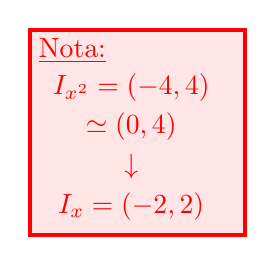
\begin{tikzpicture}[baseline=(current bounding box.center)]
                        \node[red,draw=red,fill=red!10,line width=1.5pt,text width=2.5cm] {\underline{Nota:} \\
                        $\begin{array}{c}
                              I_{x^2}=(-4,4)\\
                              \simeq(0,4)\\
                              \downarrow\\
                              I_x=(-2,2)
                        \end{array}$};
                  \end{tikzpicture}
            \end{wrapfigure}
            
            $\sum_{n=1}^{+\infty}\dfrac{(-1)^{n+1}}{(2n-1)!(2n-1)}x^{2n-1}\begin{cases}
                  x_0=0\\
                  a_n=\dfrac{(-1)^{n+1}}{(2n-1)!(2n-1)}\\
                  x^{2n-1}=\left[x^{\frac{2n-1}{n}}\right]^n\longrightarrow\text{I.C}\longrightarrow x^{\frac{2n-1}{n}}\xrightarrow[n\to+\infty]{}\bboxed{x^2}
            \end{cases}$
            
            $\rho=\lim_{n\to\infty}\left|\dfrac{a_{n+1}}{a_n}\right|=\lim_{n\to\infty}\left|\dfrac{\frac{\cancel{(-1)^{n+2}}}{(2n+1)!(2n+1)}}{\frac{\cancel{(-1)^{n+1}}}{(2n-1)!(2n-1)}}\right|=\lim_{n\to\infty}\dfrac{(2n-1)!(2n-1)}{(2n+1)!(2n+1)}=\lim_{n\to\infty}\dfrac{\cancel{(2n-1)!}(2n-1)}{(2n+1)\cdot2n\cdot\cancel{(2n-1)!}\cdot(2n+1)}=\lim_{n\to\infty}\dfrac{2n-1}{(2n+1)\cdot2n\cdot(2n+1)}=0\longrightarrow$ 
            
            $r=+\infty$
            
            $I_{x^2}=(-\infty,+\infty)\simeq(0,+\infty)\longrightarrow\bboxed{I=(-\infty,+\infty)}$
      \end{minipage}
\end{enumerate}
\item \lb{Calcular la suma:}

\begin{minipage}[l]{\textwidth}
      \begin{wrapfigure}{r}{0.35\textwidth}
            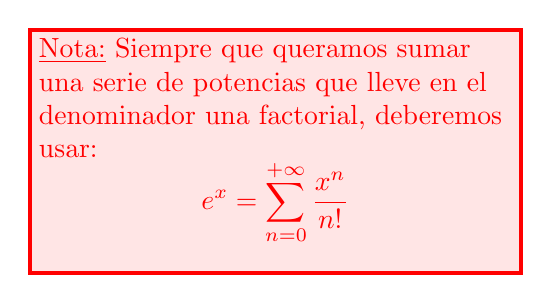
\begin{tikzpicture}[baseline=(current bounding box.center)]
                  \node[red,draw=red,fill=red!10,line width=1.5pt,text width=6cm] {\underline{Nota:} Siempre que queramos sumar una serie de potencias que lleve en el denominador una factorial, deberemos usar: \[ e^x=\sum_{n=0}^{+\infty}\dfrac{x^n}{n!} \]};
            \end{tikzpicture}
      \end{wrapfigure}
      
      $\db{\sum_{n=1}^{+\infty}\dfrac{1}{2^n\cdot n!}=}\sum_{n=1}^{+\infty}\dfrac{\left(\frac{1}{2}\right)^n}{n!}=\sum_{n=1}^{+\infty}\dfrac{x^n}{n!}=\bboxed{\sum_{n=1}^{+\infty}\dfrac{x^n}{n!}+1}-1=\sum_{n=1}^{+\infty}\dfrac{x^n}{n!}-1=e^x-1=\left\{x=\dfrac{1}{2}\right\}=e^{\frac{1}{2}}-1$
      
      $\bboxed{\sum_{n=1}^{+\infty}\dfrac{1}{2^n\cdot n!}=\sqrt{e}-1}$
\end{minipage}

\vspace{2.5cm}

\item \lb{Determinar la convergencia de la siguiente integral impropia (sin calcularla): \[ \int_{1}^{+\infty}\dfrac{\dx}{x(1+\ln(x))^p}\quad p>0 \]}

$\int_{1}^{+\infty}\dfrac{1}{x(1+\ln(x))^p}\dx=\left\{\begin{array}{l}
      1+\ln(x)=t\\
      \dfrac{1}{x}\dx=\dt\\
      \text{Si }x=1\longrightarrow t=1\\
      \text{Si }x=+\infty\longrightarrow t=+\infty
\end{array}\right\}=\int_{1}^{+\infty}\dfrac{1}{t^p}\dt=\begin{cases}
\text{Divergente si }0<p\le1\\
\text{Convergente si }p>1
\end{cases}$

\item \lb{Determinar el abierto de convergencia de las siguientes series de potencias:}

$\db{\sum_{n=1}^{\infty}\dfrac{(x-1)^n}{n4^n}=}\begin{cases}
      x_0=1\\
      a_n=\dfrac{1}{n4^n}
\end{cases}$

$\rho=\lim_{n\to\infty}\left|\dfrac{a_{n+1}}{a_n}\right|=\lim_{n\to\infty}\dfrac{\frac{1}{(n+1)\cdot4^{n+1}}}{\frac{1}{n4^n}}=\lim_{n\to\infty}\dfrac{n\cdot\cancel{4^n}}{(n+1)\cdot\cancel{4^n}\cdot4}=\lim_{n\to\infty}\dfrac{n}{4n+4}=\left(\dfrac{\infty}{\infty}\right)=\lim_{n\to\infty}\dfrac{\frac{n}{n}}{\frac{4n}{n}+\tozero{\frac{4}{n}}}=\dfrac{1}{4}\longrightarrow r=\dfrac{1}{\rho}=4\longrightarrow\bboxed{I=(x_0-r,\,x_o+r)=(-3,5 )}$

\item \lb{Determinar el abierto de convergencia de las siguientes series de potencias:}

$\db{\sum_{n=1}^{\infty}\dfrac{1}{n}\left(\dfrac{x}{2}\right)^{2}}=\sum_{n=1}^{+\infty}\dfrac{1}{n}\cdot\dfrac{x^{2n}}{2^{2n}}=\sum_{n=1}^{+\infty}\dfrac{1}{n4^n}\cdot x^{2n}\begin{cases}
      x_0=0\\
      a_n=\dfrac{1}{n4^n}\\
      x^{2n}=(x^2)^n\longrightarrow \mathrm{I.C.}(x^2)
\end{cases}$

Como $a_n=\dfrac{1}{n4^n}\longrightarrow\rho=\dfrac{1}{4}\longrightarrow r=4\longrightarrow I_{x^2}=(-4,4)\simeq[0,4)\longrightarrow\bboxed{\mathrm{I.C.}=(-2,2)}$

\item \lb{Determinar el abierto de convergencia de las siguientes series de potencias:}

$\db{\sum_{n=1}^{\infty}\dfrac{(-1)^n(x+1)^n}{n2^n}}\begin{cases}
      x_0=-1\\
      a_n=\dfrac{(-1)^n}{n2^n}
\end{cases}$

$\rho=\lim_{n\to\infty}\left|\dfrac{a_{n+1}}{a_n}\right|=\lim_{n\to\infty}\left|\dfrac{\frac{\cancel{(-1)^{n+1}}}{(n+1)\cdot 2^{n+1}}}{\frac{\cancel{(-1)^n}}{n\cdot 2^n}}\right|=\lim_{n\to\infty}\dfrac{n\cdot\cancel{2^n}}{(n+1)\cdot\cancel{2^n}\cdot2}=\lim_{n\to\infty}\dfrac{n}{2n+2}=\left(\dfrac{\infty}{\infty}\right)=\lim_{n\to\infty}\dfrac{\frac{n}{n}}{\frac{2n}{n}+\tozero{\frac{2}{n}}}=\dfrac{1}{2}$

$\rho=\dfrac{1}{2}\longrightarrow r=2\longrightarrow\mathrm{I.C.}=(-3,1)$

\item \lb{Hallar el intervalo de convergencia de: \[ \sum_{n=1}^{+\infty}\dfrac{1}{n}x^n \]Obtener la expresión de la función definida a partir de esa serie de potencias.}

$\sum_{n=1}^{+\infty}\dfrac{1}{n}\cdot x^n\begin{cases}
      x_0=0\\
      a_n=\dfrac{1}{n}
\end{cases}$

$\rho=\lim_{n\to\infty}\left|\dfrac{a_{n+1}}{a_n}\right|=\lim_{n\to\infty}\dfrac{\frac{1}{n+1}}{\frac{1}{n}}=\lim_{n\to\infty}\dfrac{n}{n+1}=\left(\dfrac{\infty}{\infty}\right)=\lim_{n\to\infty}\dfrac{\frac{n}{n}}{\frac{n}{n}+\tozero{\frac{1}{n}}}=1\longrightarrow r=1$

$\bboxed{\mathrm{I.C.}=(-1,1)}$

\begin{minipage}[l]{\textwidth}
      \begin{wrapfigure}{r}{0.3\textwidth}
            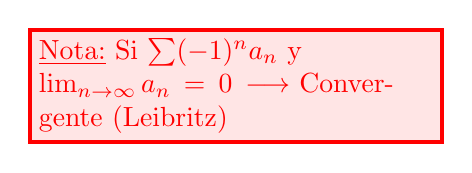
\begin{tikzpicture}[baseline=(current bounding box.center)]
                  \node[red,draw=red,fill=red!10,line width=1.5pt,text width=5cm] {\underline{Nota:} Si $\sum(-1)^na_n$ y $\lim_{n\to\infty}a_n=0\longrightarrow$ Convergente (Leibritz)};
            \end{tikzpicture}
      \end{wrapfigure}
      
      \textbullet\quad  Si $x=1\longrightarrow\sum_{n=1}^{\infty}\dfrac{1}{n}$ divergente $(p=1)$
      
      \textbullet\quad Si $x=-1\longrightarrow\sum_{n=1}^{\infty}\dfrac{(-1)^n}{n}$ convergente $\left(\lim_{n\to\infty}\dfrac{1}{n}=0\quad\mathrm{Leibritz}\right)$
      
      $\bboxed{\mathrm{I.C.}=[-1,1)}$
      
      $\sum_{n=1}^{\infty}\dfrac{1}{n}x^n=S(x)$. Como la $n$ está dividiendo, me interesa derivar, para eliminar la $n$:
      
      $S'(x)=\sum_{n=1}^{\infty}\dfrac{1}{n}\cdot nx^{n-1}\sum_{n=1}^{\infty}x^{n-1}=\lim_{n\to\infty}\lbb{\sum_{n=1}^{p}x^{n-1}}{\text{serie geométrica}}=\lim_{n\to\infty}\dfrac{1-\tozero{x^{n-1}\cdot x}}{1-x}=\dfrac{1}{1-x}$
      
      \begin{wrapfigure}{l}{0.4\textwidth}
            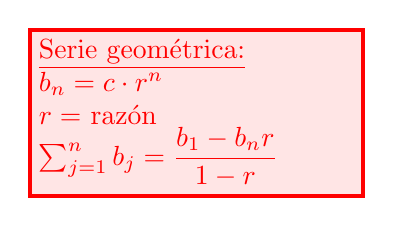
\begin{tikzpicture}[baseline=(current bounding box.center)]
                  \node[red,draw=red,fill=red!10,line width=1.5pt,text width=4cm] {\underline{Serie geométrica:}\\
                  $b_n=c\cdot r^n$\\
                  $r=$ razón\\
                  $\sum_{j=1}^{n}b_j=\dfrac{b_1-b_nr}{1-r}$};
            \end{tikzpicture}
            
            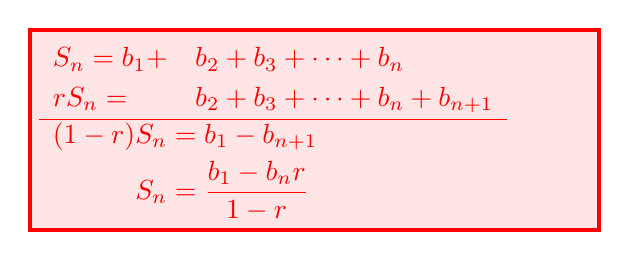
\begin{tikzpicture}[baseline=(current bounding box.center)]
                  \node[red,draw=red,fill=red!10,line width=1.5pt,text width=7cm] {$\begin{array}{ll}
                              S_n=b_1+&b_2+b_3+\cdots+b_n\\
                              rS_n= & b_2+b_3+\cdots+b_n+b_{n+1}\\ \hline
                              \multicolumn{2}{l}{\begin{aligned}
                                    (1-r)S_n&=b_1-b_{n+1}\\
                                    S_n&=\dfrac{b_1-b_nr}{1-r}
                              \end{aligned}}
                        \end{array}$};
            \end{tikzpicture}
      \end{wrapfigure}
      
      Por lo tanto: $S'(x)=\dfrac{1}{1-x}$
      
      Ahora integramos para obtener $S(x)$:
      
      $$\begin{array}{l}
            S(x)=\int\dfrac{1}{1-x}\dx=-\log(1-x)+\mathrm{C}\\
            S(x=0)=0\longrightarrow S(0)=\bboxed{C=0}\\
            \bboxed{S(x)=-\log(1-x)}
      \end{array}$$
\end{minipage}

\vspace{3.5cm}

\item \lb{Hallar las sumas de las siguientes series, estudiando en cada caso sin intervalo de convergencia:}

$\db{\sum_{n\ge1}\dfrac{x^{2n}}{2n}}$

$\sum_{n=1}^{\infty}\dfrac{1}{2n}\cdot x^{2n}\begin{cases}
      x_0=0\\
      a_n=\dfrac{1}{2n}\\
      x^{2n}=(x^2)^n\longrightarrow\mathrm{IC}(x^2)
\end{cases}$

$\rho=\lim_{n\to\infty}\left|\dfrac{a_{n+1}}{a_n}\right|=\lim_{n\to\infty}\left|\dfrac{\frac{1}{2(n+1)}}{\frac{1}{2n}}\right|=\lim_{n\to\infty}\dfrac{n}{n+1}=\lim_{n\to\infty}\dfrac{\frac{n}{n}}{\frac{n}{n}+\tozero{\frac{1}{n}}}=1\longrightarrow r=1$

$\begin{rcases}
      \mathrm{IC}_{x^2}=(-1,1)\simeq[0,1)\longrightarrow\mathrm{IC}=(-1,1)\\
      \text{Si }x=1\longrightarrow\sum_{n=1}^{\infty}\dfrac{1}{2n}\text{ Divergente }(p=1)\\
      \text{Si }x=-1\longrightarrow\sum_{n=1}^{\infty}\dfrac{(-1)^{2n}}{2n}=\sum_{n=1}^{\infty}\dfrac{1}{2n}\text{ Divergente }(p=1)
\end{rcases}\bboxed{\mathrm{IC}=(-1,1)}$

Para sumar: $S(x)=\sum_{n=1}^{\infty}\dfrac{x^{2n}}{2n}\longrightarrow S'(x)=\sum_{n=1}^{\infty}\dfrac{\cancel{(2n)}\cdot x^{2n-1}}{\cancel{2n}}=\sum_{n=1}^{\infty}x^{2n-1}=\underset{\begin{subarray}{c}
            \downarrow\\
            \text{razón $=x^2$}
\end{subarray}}{x^1+x^3+x^5+\cdots}$

$S'(x)=\sum_{n=1}^{\infty}x^{2n-1}=\dfrac{x}{1-x^2}=\dfrac{\text{1º término}}{1-\text{Razón}}\longrightarrow S'(x)=\dfrac{x}{1-x^2}$

$S(x)=\int\dfrac{x}{1-x^2}\dx=-\dfrac{1}{2}\int\dfrac{-2x}{1-x^2}\dx=-\dfrac{1}{2}\ln(1-x^2)+\mathrm{C}$

$S(0)=\bboxed{\mathrm{C}=0}\longrightarrow\bboxed{S(x)=-\dfrac{1}{2}\ln(1-x^2)}$

\item \lb{Hallar las sumas de las siguientes series, estudiando en cada caso su intervalo de convergencia:}

$\db{\sum_{n\ge1}\dfrac{x^{4n-1}}{4n-1}}$

$\sum_{n=1}^{\infty}\dfrac{x^{4n-1}}{4n-1}=\begin{cases}
      x_0=0\\
      a_n=\dfrac{1}{4n-1}\\
      x^{4n-1}=\left[x^{\frac{4n-1}{n}}\right]^n\xrightarrow[n\to+\infty]{}x^4\leadsto I_{x^4}
\end{cases}$

$\rho=\lim_{n\to\infty}\left|\dfrac{a_{n+1}}{a_n}\right|=\lim_{n\to\infty}\left|\dfrac{\frac{1}{4n+3}}{\frac{1}{4n-1}}\right|=\lim_{n\to\infty}\dfrac{4n-1}{4n+3}=\left(\dfrac{\infty}{\infty}\right)=\lim_{n\to\infty}\dfrac{\frac{4n}{n}-\tozero{\frac{1}{n}}}{\frac{4n}{n}+\tozero{\frac{3}{n}}}=1$

$\begin{rcases}
      \rho=1\longrightarrow r=\dfrac{1}{\rho}=1\longrightarrow\bboxed{I=(-1,1)}\\
      \text{Si }x=1\longrightarrow\sum_{n=1}^{\infty}\dfrac{1}{4n-1}\text{ Divergente }\left(\sum\dfrac{1}{n}\right)\\
      \text{Si }x=-1\longrightarrow\sum_{n=1}^{\infty}\dfrac{-1}{4n-1}\text{ Divergente }
\end{rcases}I_{x^4}\simeq[0,1)\longrightarrow\bboxed{I=(-1,1)}$

Definimos: $S(x)=\sum_{n=1}^{\infty}\dfrac{x^{4n-1}}{4n-1}\longrightarrow S'(x)=\dfrac{\cancel{(4n-1)}x^{4n-2}}{\cancel{4n-1}}$

$S'(x)=\sum_{n=1}^{\infty}x^{4n-2}=\underset{\begin{subarray}{c}
            \downarrow\\
            \text{Razón}=x^4
\end{subarray}}{x^2+x^6+x^{10}+\cdots}=\dfrac{x^2}{1-x^4}$

Por lo tanto: $S(x)=\int\dfrac{x^2}{1-x^4}\dx=\int\dfrac{x^2}{(1-x^2)(1+x^2)}\dx=\int\dfrac{x^2}{(1-x)(1+x)(1+x^2)}\dx=\lb{(\ast)}$

$\dfrac{x^2}{(1-x)(1+x)(1+x^2)}=\dfrac{A}{1-x}+\dfrac{B}{1+x}+\dfrac{Cx+D}{1+x^2}=\dfrac{A(1+x)(1+x^2)+B(1-x)(1+x^2)+(Cx+D)(1-x)(1+x)}{(1-x)(1+x)(1+x^2)}$

$\begin{array}{l}
      x^2=A(1+x)(1+x^2)+B(1-x)(1+x^2)+(Cx+D)(1-x)(1+x)\\
      \text{Si }x=1\longrightarrow1=4A\longrightarrow A=\dfrac{1}{4}\\
      \text{Si }x=-1\longrightarrow1=4B\longrightarrow B=\dfrac{1}{4}\\
      \text{Si }x=0\longrightarrow0=\dfrac{1}{4}+\dfrac{1}{4}+D\longrightarrow D=-\dfrac{1}{2}\\
      \text{Si }x=2\longrightarrow4=\dfrac{15}{4}-\dfrac{5}{4}+\left(2C-\dfrac{1}{2}\right)(-3)=\longrightarrow\dfrac{3}{2}=-3\left(2C-\dfrac{1}{2}\right)\longrightarrow-\dfrac{1}{2}=2C-\dfrac{1}{2}\longrightarrow\bboxed{C=0}
\end{array}$

$\lb{(\ast)=}\int\dfrac{1}{4}\cdot\dfrac{1}{1-x}+\dfrac{1}{4}\cdot\dfrac{1}{1+x}-\dfrac{1}{2}\cdot\dfrac{1}{1+x^2}\dx=-\dfrac{1}{4}\ln|1-x|+\dfrac{1}{4}\ln|1+x|-\dfrac{1}{2}\arctan(x)$

$\bboxed{\sum_{n=1}^{\infty}\dfrac{x^{4n-1}}{4n-1}=-\dfrac{1}{4}\ln|1-x|+\dfrac{1}{4}\ln|1+x|-\dfrac{1}{2}\arctan(x)}$

\item \lb{Hallar las sumas de las series, estudiando en cada caso su intervalo de convergencia:}

$\db{\sum_{n=0}^{\infty}\dfrac{x^{n+2}}{(n+2)n!}=}\begin{cases}
      x_0=0\\
      a_n=\dfrac{1}{(n+2)n!}\\
      x^{n+2}=\underset{\begin{subarray}{c}
                  \downarrow\\
                  x^1
      \end{subarray}}{\left[x^{\frac{n+2}{n}}\right]^n}\longrightarrow x\longrightarrow I_x
\end{cases}$

$\rho=\lim_{n\to\infty}\left|\dfrac{a_{n+1}}{a_n}\right|=\lim_{n\to\infty}\dfrac{\frac{1}{(n+3)(n+1)!}}{\frac{1}{(n+2)n!}}=\lim_{n\to\infty}\dfrac{(n+2)\cdot\cancel{n!}}{(n+3)(n+1)\cdot\cancel{n!}}=\lim_{n\to\infty}\dfrac{n+2}{n^2+4n+3}=0$

$r=+\infty\longrightarrow\bboxed{I=(-\infty,+\infty)=\R}$

\begin{minipage}[l]{\textwidth}
      \begin{wrapfigure}{r}{0.35\textwidth}
            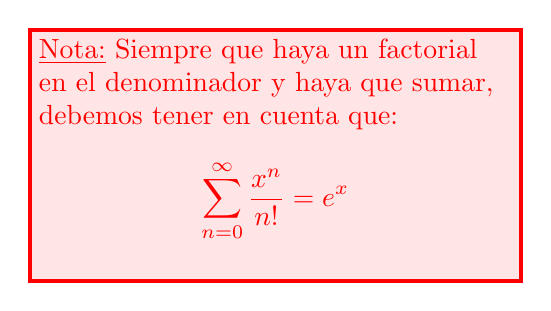
\begin{tikzpicture}[baseline=(current bounding box.center)]
                  \node[red,draw=red,fill=red!10,line width=1.5pt,text width=6cm] {\underline{Nota:} Siempre que haya un factorial en el denominador y haya que sumar, debemos tener en cuenta que: \[\sum_{n=0}^{\infty}\dfrac{x^n}{n!}=e^x  \]};
            \end{tikzpicture}
      \end{wrapfigure}

Sea $S(x)=\sum_{n=0}^{\infty}\dfrac{x^{n+2}}{(n+2)n!}\longrightarrow S'(x)=\sum_{n=0}^{\infty}\dfrac{\cancel{(n+2)}x^{n+1}}{\cancel{(n+2)}n!}=\sum_{n=0}^{\infty}\dfrac{x^{n+1}}{n!}=x\cdot\sum_{n=0}^{\infty}\dfrac{x^n}{n!}=xe^x$

$S(x)\int xe^x\dx=\left\{\begin{array}{ll}
      u=x & \du=\dx\\
      \dv=e^x\dx & v=e^x
\end{array}\right\}=xe^x-\int e^x\dx=xe^x-e^x+\mathrm{C}$

$S(x=0)=0\longrightarrow S(x=0)=-1+\mathrm{C}=0\longrightarrow\bboxed{\mathrm{C}=1}$

$\bboxed{S(x)=e^x(x-1)+1}$
\end{minipage}
\item \lb{Hallar las sumas de las siguientes series, estudiando en cada caso su intervalo de convergencia:}

$\db{\sum_{n=1}^{\infty}nx^n}\begin{cases}
      x_0=0\\
      a_n=n
\end{cases}$

$\rho=\lim_{n\to\infty}\left|\dfrac{a_{n+1}}{a_n}\right|=\lim_{n\to\infty}\dfrac{n+1}{n}=\lim_{n\to\infty}\left(1+\dfrac{1}{n}\right)=1\longrightarrow r=1$

$\begin{rcases}
      I=(-1,1)\\
      \text{Si }x=1\longrightarrow\sum_{n=1}^{\infty}n\text{ divergente}\\
      \text{Si }x=-1\longrightarrow\sum_{n=1}^{\infty}(-1)^nn\text{ divergente}
\end{rcases}\bboxed{I=(-1,1)}$

Sea $S(X)=\sum_{n=1}^{\infty}nx^n=x\cdot\lbb{\sum_{n=1}^{\infty}nx^{n-1}}{T(x)}$

$\int T(x)\dx=\sum_{n=1}^{\infty}\cancel{n}\cdot\dfrac{x^n}{\cancel{n}}=\sum_{n=1}^{\infty}x^n=\underset{\begin{subarray}{c}
            \downarrow\\
            \text{Razón}=x
\end{subarray}}{x+x^2+x^3+x^4+\cdots}=\dfrac{x}{1-x}$

$T(x)=\left(\dfrac{x}{1-x}\right)'=\dfrac{(1-x)+x}{(1-x)^2}=\dfrac{1}{(1-x)^2}\longrightarrow\bboxed{S(x)=\dfrac{x}{(1-x)^2}}$

\item \lb{Hallar las sumas de las siguientes series, estudiando en cada caso su intervalo de convergencia:}

$\db{\sum_{n=1}^{\infty}n^2x^n=}\begin{cases}
      x_0=0\\
      a_n=n^2
\end{cases}$

$\rho=\lim_{n\to\infty}\left|\dfrac{a_{n+1}}{a_n}\right|=\lim_{n\to\infty}\dfrac{(n+1)^2}{n^2}=\lim_{n\to\infty}\left(\dfrac{n}{n}+\tozero{\dfrac{1}{n}}\right)^2=1\longrightarrow r=1$

$\begin{rcases}
      I=(-1,1)\\
      \text{Si }x=1\longrightarrow\sum_{n=1}^{\infty}n^2\text{ Divergente}\\
      \text{Si }x=-1\longrightarrow\sum_{n=1}^{\infty}(-1)^n\cdot n^2\text{ Divergente}
\end{rcases}\bboxed{I=(-1,1)}$

Sea $S(x)=\sum_{n=1}^{\infty}n^2x^n=x\cdot\lbb{\sum_{n=1}^{\infty}n^2x^{n-1}}{T(x)}$

$\int T(x)=\sum_{n=1}^{\infty}n^2\cdot\dfrac{x^n}{n}=\sum_{n=1}^{\infty}nx^n=x\cdot\dbb{\sum_{n=1}^{\infty}nx^{n-1}}{R(x)}$

$\int R(x)=\sum_{n=1}^{\infty}n\dfrac{x^n}{n}=\sum_{n=1}^{\infty}x^n=\underset{\begin{subarray}{c}
            \downarrow\\
            \text{Razón}=x
\end{subarray}}{x+x^2+x^3+x^4+\cdots}=\dfrac{x}{1-x}$

Echamos marcha atrás:

$R(x)=\left(\dfrac{x}{1-x}\right)'=\dfrac{1-x+x}{(1-x)^2}=\dfrac{1}{1-x^2}\longrightarrow\int T(x)\dx=\dfrac{x}{(1-x)^2}$

$T(x)=\left(\dfrac{x}{(1-x)^2}\right)'=\dfrac{(1-x)^{\cancel{2}}+2\cancel{(1-x)}\cdot x}{(1-x)^{\cancel{4}\lb{3}}}=\dfrac{1-x+2x}{(1-x)^3}=\dfrac{x+1}{(1-x)^3}$

$\bboxed{S(x)=\dfrac{x(x+1)}{(1-x)^3}}$

\item \lb{Obtener el desarrollo de McLaurin de orden 4 de la función $f(x)=\log(1+x)$. Utilizarlo para dar un valor aproximado de $\log(1.2)$ y proporcionar una cota del error cometido en la aproximación.}

Desarrollo de McLaurin$\longrightarrow$ Taylor con $a=0$. \[ T_4(x)=f(0)+\dfrac{f'(0)}{1!}x+\dfrac{f''(0)}{2!}x^2+\dfrac{f'''(0)}{3!}x^3+\dfrac{f^{\mathrm{iv}}(0)}{4!}x^4 \]

$\begin{array}{l}
      f(x)=\log(1+x)\longrightarrow f(0)=0\\
      f'(x)=\dfrac{1}{1+x}=(1-x)^{-1}\longrightarrow f'(0)=1\\
      f''(x)=(-1)(1+x)^{-2}=\dfrac{1}{(1+x)^2}\longrightarrow f''(0)=-1\\
      f'''(x)=2(1+x)^{-3}=\dfrac{2}{(1+x)^3}\longrightarrow f'''(0)=2\\
      f^{\mathrm{iv}}(x)=-6(1+x)^{-4}=\dfrac{-6}{(1+x)^4}\longrightarrow f^{\mathrm{iv}}(0)=-6\\
      f^{\mathrm{v}}(x)=24(1+x)^{-5}=\dfrac{24}{(1+x)^5}
\end{array}\qquad\begin{array}{l}
T_4(x)=x-\dfrac{1}{2}x^2+\dfrac{2}{6}x^3-\dfrac{6}{24}x^4\\
\\
\bboxed{T_4(x)=x-\dfrac{1}{2}x^2+\dfrac{1}{3}x^3-\dfrac{1}{4}x^4}
\end{array}$

Si queremos utilizarlo para dar un valor aproximado de $\log(1.2)$, siendo la función $f(x)=\log(1+x)$, es porque \[ \log(1+x)=\log(1.2)\longrightarrow1+x=1.2\longrightarrow\bboxed{x=0.2} \]
Por lo tanto, debemos tomar el desarrollo obtenido y sustituir la $x=0.2$: \[ \log(1.2)\simeq0.2-\dfrac{1}{2}(0.2)^2+\dfrac{1}{3}(0.2)^3-\dfrac{1}{4}(0.2)^4=0.18226\longrightarrow\bboxed{\log(1.2)\simeq0.18226} \]

Para poder dar una cota del error cometido en la aproximación lo que haremos será utilizar la expresión del resto de Lagrange:

$R_4(x)=\underset{a<c<x}{\left|\dfrac{f^{\mathrm{iv}}(c)}{5!}(x-a)^5\right|}=\underset{0<c<0.2}{\left|\dfrac{\frac{24}{(1+c)^5}}{120}(0.2)^5\right|}=\dfrac{1}{5(1+c)^5}(0.2)^5\underset{\begin{subarray}{c}
            \downarrow\\
            \text{acotamos el valor}\\
            \text{de $c$ por cero}
\end{subarray}}{<}\dfrac{1}{5}(0.2)^5=6.4\cdot10^{-5}$

\fcolorbox{lightblue}{lightblue!10}{El error máximo cometido en la aproximación viene dado por $E<6.4\cdot10^{-5}$}
\pagebreak
\item \lb{Calcular un valor aproximado de $\sin(0.2)$ con un error menor de $10^{-4}$.}

\begin{minipage}[l]{\textwidth}
      \begin{wrapfigure}[2]{r}{0.5\textwidth}
            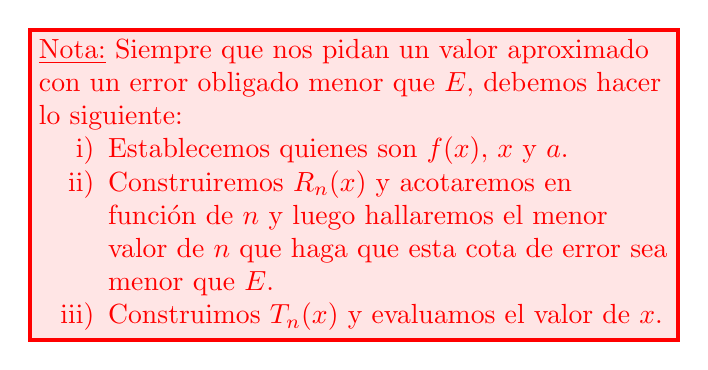
\begin{tikzpicture}[baseline=(current bounding box.center)]
                  \node[red,draw=red,fill=red!10,line width=1.5pt,text width=8cm] {\underline{Nota:} Siempre que nos pidan un valor aproximado con un error obligado menor que $E$, debemos hacer lo siguiente: 
                  
                  \begin{enumerate}[label=\roman*)]
                        \item Establecemos quienes son $f(x),\, x$ y $a$.
                        \item Construiremos $R_n(x)$ y acotaremos en función de $n$ y luego hallaremos el menor valor de $n$ que haga que esta cota de error sea menor que $E$.
                        \item Construimos $T_n(x)$ y evaluamos el valor de $x$.
                        \end{enumerate}};
            \end{tikzpicture}
      \end{wrapfigure}
      
      Tomaremos $f(x)=\sin(x)$ con $x=0.2$ y $a=0$.
      
      $\begin{array}{l}
            f(x)\sin(x)\\
            f'(x)=\cos(x)\\
            f''(x)=-\sin(x)\\
            f'''(x)=-\cos(x)\\
            f^{\mathrm{iv}}(x)=\sin(x)\\
            \vdots\\
            \left|f^n(x)\right|\le1
      \end{array}$
      
      \vspace{1.5cm}
      
      $R_n(x)=\left|\dfrac{f^{n+1}(c)}{(n+1)!}(x-a)^{n+1}\right|=\dfrac{\left|f^{(n+1)(c)}\right|}{(n+1)!}(0.2)^{n+1}\le\lbb{\dfrac{1}{(n+1)!}(0.2)^{n+1}}{E_n}<10^{-4}$
\end{minipage}
\begin{itemize}
      \item Si $n=4\longrightarrow E_4=2.666\cdot10^{-6}<10^{-4}$
      \item Si $\boxed{n=3}\longrightarrow E_3=6.66\cdot10^{-5}<10^{-4}$
      \item Si $n=2\longrightarrow E_2=1.33\cdot10^{-3}\nless10^{-4}$
\end{itemize}
Construiremos el desarrollo de Taylor en $a=0$ hasta orden 3. 

$\begin{array}{l}
      T_3(x)=f(0)+\dfrac{f(0)}{1!}x+\dfrac{f''(0)}{2!}x^2+\dfrac{f'''(0)}{3!}x^3\\
      f(0)=0;\;f'(0)=1;\;f''(0)=0;\;f'''(0)=-1\\
      \bboxed{T_3(x)=x-\dfrac{1}{6}x^3}\\
      T_3(x=0.2)=0.2-\dfrac{1}{6}(0.2)^3=0.189667\longrightarrow\bboxed{\sin(0.2)\simeq0.189667}
\end{array}$
\item \lb{Calcular:}

$\db{\int_{0}^{+\infty}\dfrac{1}{a^2+x^2}\dx=}\lim_{n\to\infty}\int_0^t\dfrac{1}{x^2+a^2}\dx=\lb{(\ast)}$

Calcularemos la primitiva:

$\int\dfrac{1}{x^2+a^2}\dx=\int\dfrac{\frac{1}{a^2}}{\frac{x^2}{a^2}+1}\dx=\dfrac{1}{a^2}\int\dfrac{1}{\left(\frac{x}{a}\right)^2+1}\dx=\dfrac{a}{a^2}\int\dfrac{\frac{1}{a}}{\left(\frac{x}{a}\right)^2+1}\dx=\left\{\begin{array}{l}
      \dfrac{x}{a}=u\\
      \dfrac{1}{a}\dx=\du
\end{array}\right\}=\dfrac{1}{a}\int\dfrac{1}{u^2+1}\du=\dfrac{1}{a}\arctan(u)=\dfrac{1}{a}\arctan\left(\dfrac{x}{a}\right)$

$\lb{(\ast)=}\lim_{t\to+\infty}\left[\dfrac{1}{a}\arctan\left(\dfrac{x}{a}\right)\right]_0^t=\lim_{t\to+\infty}\dfrac{1}{a}\left[\arctan\left(\dfrac{t}{a}\right)-0\right]=\dfrac{1}{a}\arctan(+\infty)=\dfrac{1}{a}\cdot\dfrac{\pi}{2}=\bboxed{\dfrac{\pi}{2a}}$
\pagebreak
\item \lb{Hallar el área de la región acotada por las curvas $y_1=2x^3-x^2-5x$ e $y=-x^2+3x$.}

\begin{minipage}[l]{\textwidth}
      \begin{wrapfigure}{r}{0.5\textwidth}
            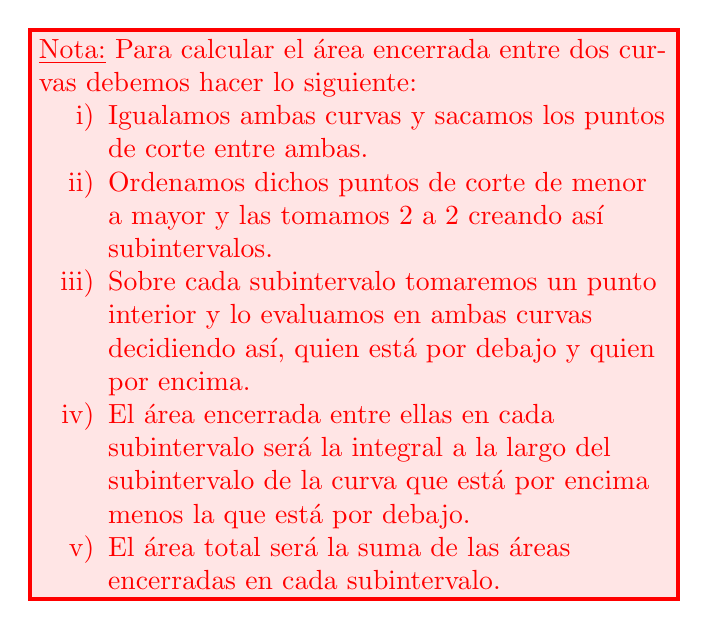
\begin{tikzpicture}[baseline=(current bounding box.center)]
                  \node[red,draw=red,fill=red!10,line width=1.5pt,text width=8cm] {\underline{Nota:} Para calcular el área encerrada entre dos curvas debemos hacer lo siguiente:
                  \begin{enumerate}[label=\roman*)]
                        \item Igualamos ambas curvas y sacamos los puntos de corte entre ambas.
                        \item Ordenamos dichos puntos de corte de menor a mayor y las tomamos 2 a 2 creando así subintervalos.
                        \item Sobre cada subintervalo tomaremos un punto interior y lo evaluamos en ambas curvas decidiendo así, quien está por debajo y quien por encima.
                        \item El área encerrada entre ellas en cada subintervalo será la integral a la largo del subintervalo de la curva que está por encima menos la que está por debajo.
                        \item El área total será la suma de las áreas encerradas en cada subintervalo.
                        \end{enumerate}};
            \end{tikzpicture}
      \end{wrapfigure}
      
      $\begin{rcases}
            y_1=2x^3-x^2-5x\\
            y_2=-x^2+3x
      \end{rcases}2x^3\cancel{x^2}-5x=\cancel{-x^2}+3x\longrightarrow2x^3-8x=0\longrightarrow x(2x^2-8)=0$
      
      $\begin{array}{l}
            \bboxed{x=0}\\
            2x^2-8=0\longrightarrow x^2=4\longrightarrow\bboxed{x=\pm2}
      \end{array}$
      
      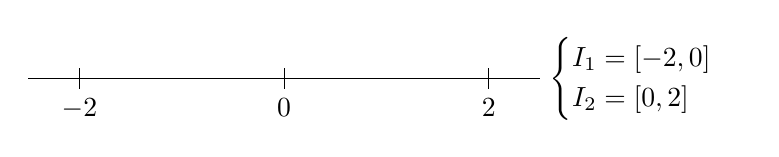
\begin{tikzpicture}[scale=1.3]
            \draw (-2.5,0) -- (2.5,0) node[right] {$\begin{cases}
                        I_1=[-2,0]\\
                        I_2=[0,2]
                  \end{cases}$};
            \foreach \x in {-2,0,2}{
            \draw (\x,0.1) -- (\x,-0.1) node[below] {$\x$};
            }
      \end{tikzpicture}
      
      $\begin{array}{ll}
            I_1=[-2,0] & y_1(-1)=2\\
            & y_2(-1)=-4
      \end{array}$
      
      $A_1=\int_{-2}^{0}(2x^3-\cancel{x^2}-5x)-(\cancel{-x^2}+3x)\dx=\int_{-2}^{0}2x^3-8x\dx=\left[\dfrac{2x^4}{4}-4x^2\right]_{-2}^0=-(8-16)=8$
      
      $\begin{array}{ll}
            I_2=[0,2] & y_1(1)=-4\\
            & y_2(1)=2
      \end{array}$
      
      $A_2=\int_{0}^{2}(\cancel{-x^2}+3x)-(2x^3-\cancel{x^2}-5x)\dx=\int_{0}^{2}-2x^3+8x\dx=\left[-\dfrac{2x^4}{4}+4x^2\right]_0^2=-8+16=8$
      
      $\bboxed{A_T=A_1+A_2=16}$
\end{minipage}
\item \lb{Hallar el área limitada por las curvas $x+4y^2=4$ y $x+y^4=1$ para $x\ge0$.}

$\begin{array}{l}
      x_1=4-4y^2\\
      x_2=1-y^4
\end{array}\qquad\bboxed{x\ge0}\longrightarrow\begin{cases}
4-4y^2\ge0\longrightarrow y^2\le1\longrightarrow-1\le y\le1\\
1-y^4\ge0\longrightarrow y^4\le1\longrightarrow-1\le y\le1
\end{cases}$

$4-4y^2=1-y^4$

$y^4-4y^2+3=0\:(y^2=w)\longrightarrow w^2-4w+3=0\begin{cases}
      w=1=y^2\longrightarrow y=\pm1\\
      w=3=y^2\longrightarrow\bboxed{y=\pm\sqrt{3}}\:\lb{\begin{subarray}{l}
                  \text{No cuenta porque está}\\ \text{fuera de nuestro estudio}
      \end{subarray}}
\end{cases}$

\begin{center}
      \begin{tikzpicture}[scale=3]
            \draw (-1.5,0) -- (1.5,0);
            \foreach \x in {-1,1}{
            \draw (\x,0.1) -- (\x,-0.1) node[below] {$\x$};
            }
      \end{tikzpicture}      
\end{center}

$\begin{array}{l}
x_1(0)=4\\
x_2(0)=1
\end{array}$

$A=\int_{-1}^{1}(4-4y^2)-(1-y^4)\dy=\left[4y-\dfrac{4y^3}{3}-y+\dfrac{y^5}{5}\right]_{-1}^1=\left(4-\dfrac{4}{3}-1+\dfrac{1}{5}\right)-\left(-4+\dfrac{4}{3}+1-\dfrac{1}{5}\right)=\left(\dfrac{5}{3}+\dfrac{1}{5}\right)-\left(-\dfrac{5}{3}-\dfrac{1}{5}\right)=\dfrac{10}{3}+\dfrac{2}{5}=\bboxed{\dfrac{56}{15}}$
\pagebreak
\item \lb{Calcular el área de una elipse de semiejes $a$ y $b$.}

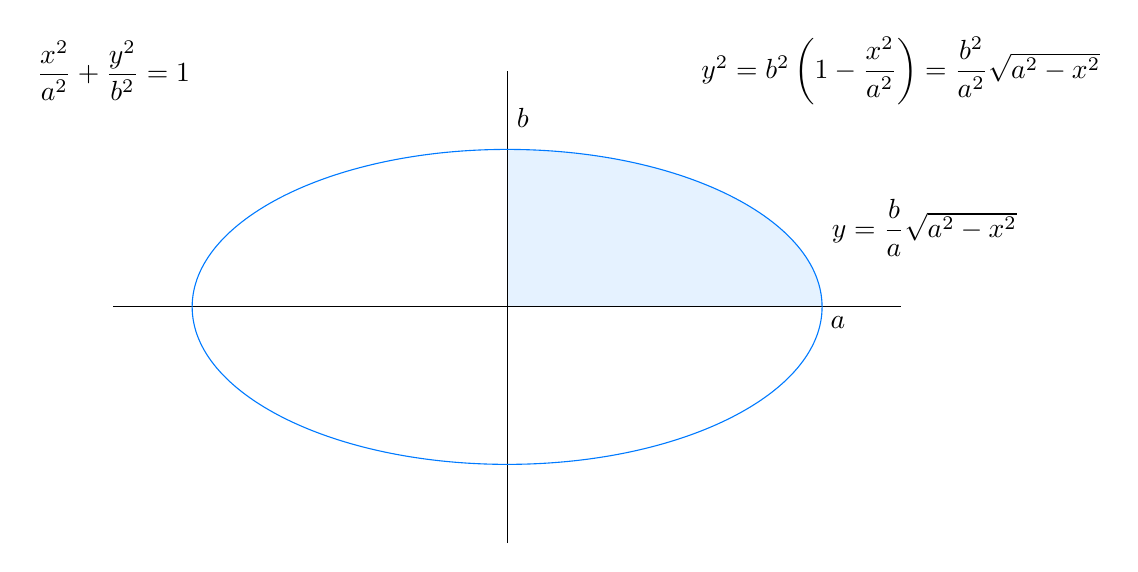
\begin{tikzpicture}[scale=2]
      \fill[lightblue!10] (0,0) -- (2,0) arc (0:90:2cm and 1cm)  -- (0,0);
      \draw (-2.5,0) -- (2.5,0);
      \draw (0,-1.5) -- (0,1.5);
      \draw[lightblue] (0,0) ellipse (2cm and 1cm) ;
      \node[right] at (0,1.2) {$b$};
      \node[below] at (2.1,0) {$a$};
      \node at (-2.5,1.5) {$\dfrac{x^2}{a^2}+\dfrac{y^2}{b^2}=1$};
      \node at (2.5,1.5) {$y^2=b^2\left(1-\dfrac{x^2}{a^2}\right)=\dfrac{b^2}{a^2}\sqrt{a^2-x^2}$};
      \node[right] at (2,0.5) {$y=\dfrac{b}{a}\sqrt{a^2-x^2}$};
\end{tikzpicture}

\begin{minipage}[l]{\textwidth}
      \begin{wrapfigure}[2]{r}{0.3\textwidth}
            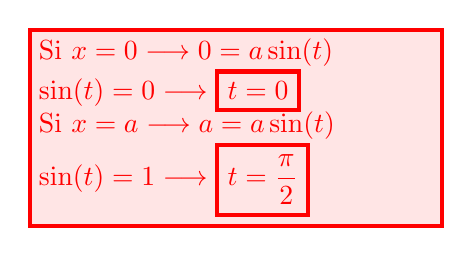
\begin{tikzpicture}[baseline=(current bounding box.center)]
                  \node[red,draw=red,fill=red!10,line width=1.5pt,text width=5cm] {Si $x=0\longrightarrow0=a\sin(t)$\\
                  $\sin(t)=0\longrightarrow\boxed{t=0}$\\
                  Si $x=a\longrightarrow a=a\sin(t)$\\
                  $\sin(t)=1\longrightarrow\boxed{t=\dfrac{\pi}{2}}$};
            \end{tikzpicture}
      \end{wrapfigure}
      
      $A=4\int_0^a\dfrac{b}{a}\sqrt{a^2-x^2}\dx=\dfrac{4b}{a}\int_0^a\sqrt{a^2-a^2}\dx=\left\{\begin{array}{l}
            x=a\sin(t)\\
            \dx=a\cos(t)\dt\\
            \text{Si }x=0\longrightarrow t=0\\
            \text{Si }x=a\longrightarrow t=\dfrac{\pi}{2}
      \end{array}\right\}=\dfrac{4b}{a}\int_{0}^{\frac{\pi}{2}}\sqrt{a^2-a^2\sin^2(t)}\cdot a\cos(t)\dt=\dfrac{4b}{a}\int_{0}^{\frac{\pi}{2}}\sqrt{a^2(1-\sin^2(t))}\cdot a\cos(t)\dt=\dfrac{4b}{\cancel{a}}\int_{0}^{\frac{\pi}{2}}\cancel{a}\cos(t)\cdot a\cos(t)\dt=4ab\int_{0}^{\frac{\pi}{2}}\cos^2(t)\dt=\left\{\cos^2(t)=\dfrac{1+\cos(2t)}{2}\right\}=4ab\int_{0}^{\frac{\pi}{2}}\dfrac{1+\cos(2t)}{2}\dt=2ab\left[t+\tozero{\dfrac{\sin(2t)}{2}}\right]_0^{\frac{\pi}{2}}=2ab\cdot\dfrac{\pi}{2}=\bboxed{\pi ab}$
\end{minipage}
\item \lb{La base de un sólido es el triángulo de vértices (0,0), (0,1) y (1,1) en el plano $XOY$. Sus secciones por planos perpendiculares al eje $OX$ son cuadrados. Calcular el volumen del sólido.}

\begin{center}
      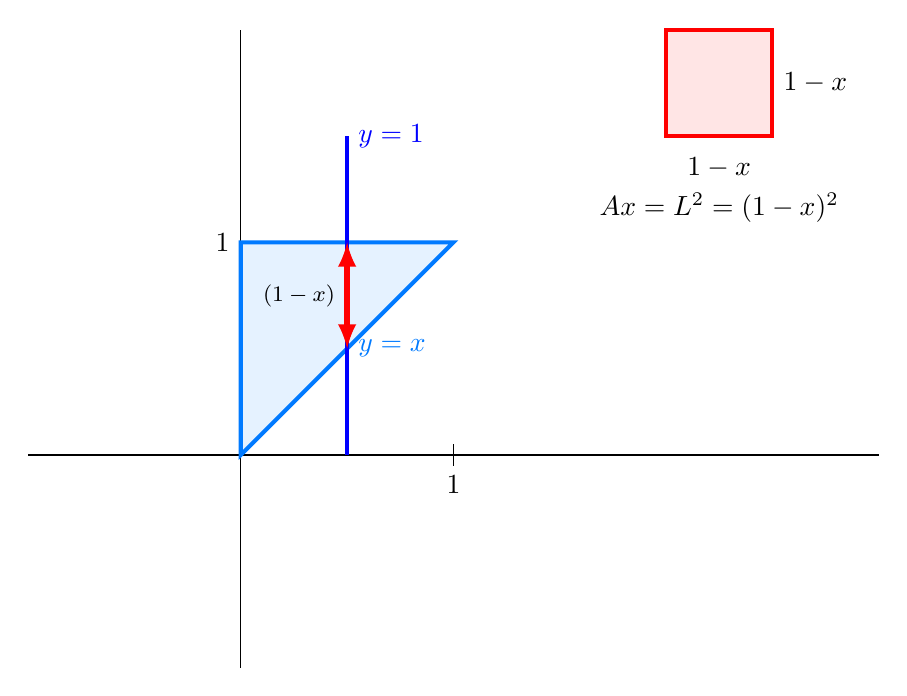
\begin{tikzpicture}[scale=2.7, >=latex]
      \draw (-1,0) -- (3,0);
      \draw (0,-1) -- (0,2);
      \draw[draw=lightblue, fill=lightblue!10, line width=1.5pt] (0,0) -- (1,1) node[midway,right] {$\lb{y=x}$} -- (0,1) node[left] {$1$} -- cycle;
      \draw[blue, line width=1.5pt] (0.5,0) -- (0.5, 1.5) node[right] {$y=1$};
      \draw[draw=red, <->, line width=2] (0.5, 0.5) -- (0.5,1) node[midway, left] {\footnotesize$(1-x)$};
      \draw (1,0.05) -- (1,-0.05) node[below] {1};
      \draw[draw=red, fill=red!10, line width=1.5] (2,2) -- (2.5,2)  -- (2.5,1.5) node[midway, right] {$1-x$} -- (2,1.5) node[midway, below] {$\begin{array}{c}
                  1-x\\
                  Ax=L^2=(1-x)^2
            \end{array}$} -- cycle;
\end{tikzpicture}
\end{center}
$\begin{array}{l}
      V=\int_0^1Ax\dx=\int_0^1(1-x)^2\dx=\left[-\dfrac{(1-x)^3}{3}\right]_0^1=\bboxed{\dfrac{1}{3}}\\
      Ax=(1-x)^2
\end{array}$

\item \lb{La base de un sólido es el triángulo de vértices (0,0), (0,1) y (1,1) en el plano $XOY$. Sus secciones por planos perpendiculares al eje $OX$ son triángulos equilateros. Calcular el volumen del sólido.}

\begin{center}
      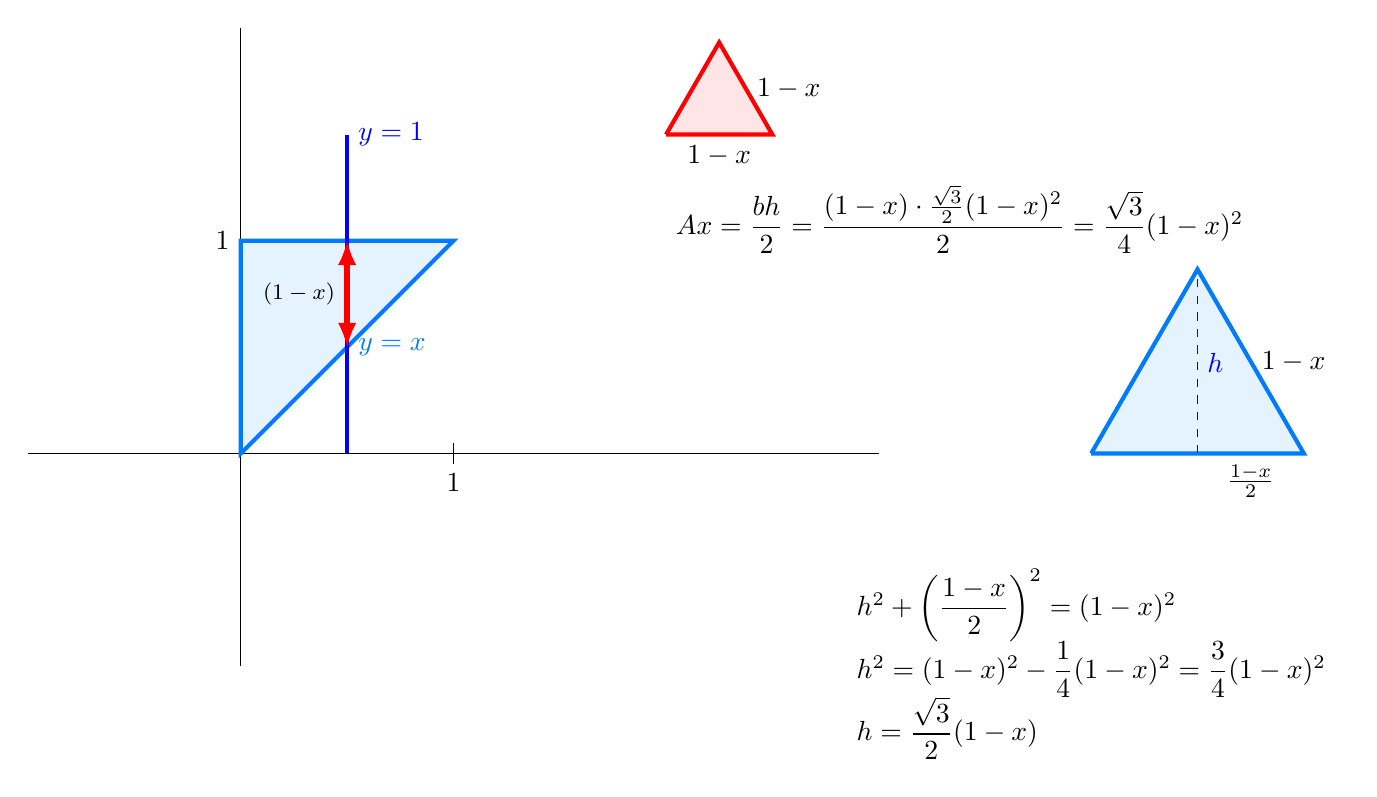
\begin{tikzpicture}[scale=2.7, >=latex]
            \draw (-1,0) -- (3,0);
            \draw (0,-1) -- (0,2);
            \draw[draw=lightblue, fill=lightblue!10, line width=1.5pt] (0,0) -- (1,1) node[midway,right] {$\lb{y=x}$} -- (0,1) node[left] {$1$} -- cycle;
            \draw[blue, line width=1.5pt] (0.5,0) -- (0.5, 1.5) node[right] {$y=1$};
            \draw[draw=red, <->, line width=2] (0.5, 0.5) -- (0.5,1) node[midway, left] {\footnotesize$(1-x)$};
            \draw (1,0.05) -- (1,-0.05) node[below] {1}; 
            \draw[draw=red, fill=red!10, line width=1.5pt] (2,1.5) -- ++(60:0.5)  -- ++(-60:0.5)  node[midway, right] {$1-x$} -- (2,1.5) node[midway, below] {$1-x$};
            \node[right] at (2, 1.1) {$Ax=\dfrac{bh}{2}=\dfrac{(1-x)\cdot\frac{\sqrt{3}}{2}(1-x)^2}{2}=\dfrac{\sqrt{3}}{4}(1-x)^2$};
            \draw[draw=lightblue, fill=lightblue!10, line width=1.5] (4,0) -- ++(60:1) -- ++(-60:1) node[midway,right] {$1-x$} -- (4.5,0) node[midway,below] {$\frac{1-x}{2}$} -- (4,0);
            \draw[blue, dashed] (4.5,0) -- (4.5,0.85) node[right, midway] {$h$};
            \node[below] at (4,-0.5) {$\begin{array}{l}
                        h^2+\left(\dfrac{1-x}{2}\right)^2=(1-x)^2\\
                        h^2=(1-x)^2-\dfrac{1}{4}(1-x)^2=\dfrac{3}{4}(1-x)^2\\
                        h=\dfrac{\sqrt{3}}{2}(1-x)
            \end{array}$};
      \end{tikzpicture} 
\end{center}
$V=\int_0^1\dfrac{\sqrt{3}}{4}(1-x)^2\dx=\dfrac{\sqrt{3}}{4}\left[-\dfrac{(1-x)^3}{3}\right]_0^1=\dfrac{\sqrt{3}}{4}\cdot\dfrac{1}{3}=\bboxed{\dfrac{\sqrt{3}}{12}}$
\item \lb{La base de un sólido es el círculo de centro (0,0) y radio 1 en el plano $XOY$. Sus secciones por planos perpendiculares al eje $OX$ son cuadrados. Calcular el volumen del sólido.}

\begin{center}
      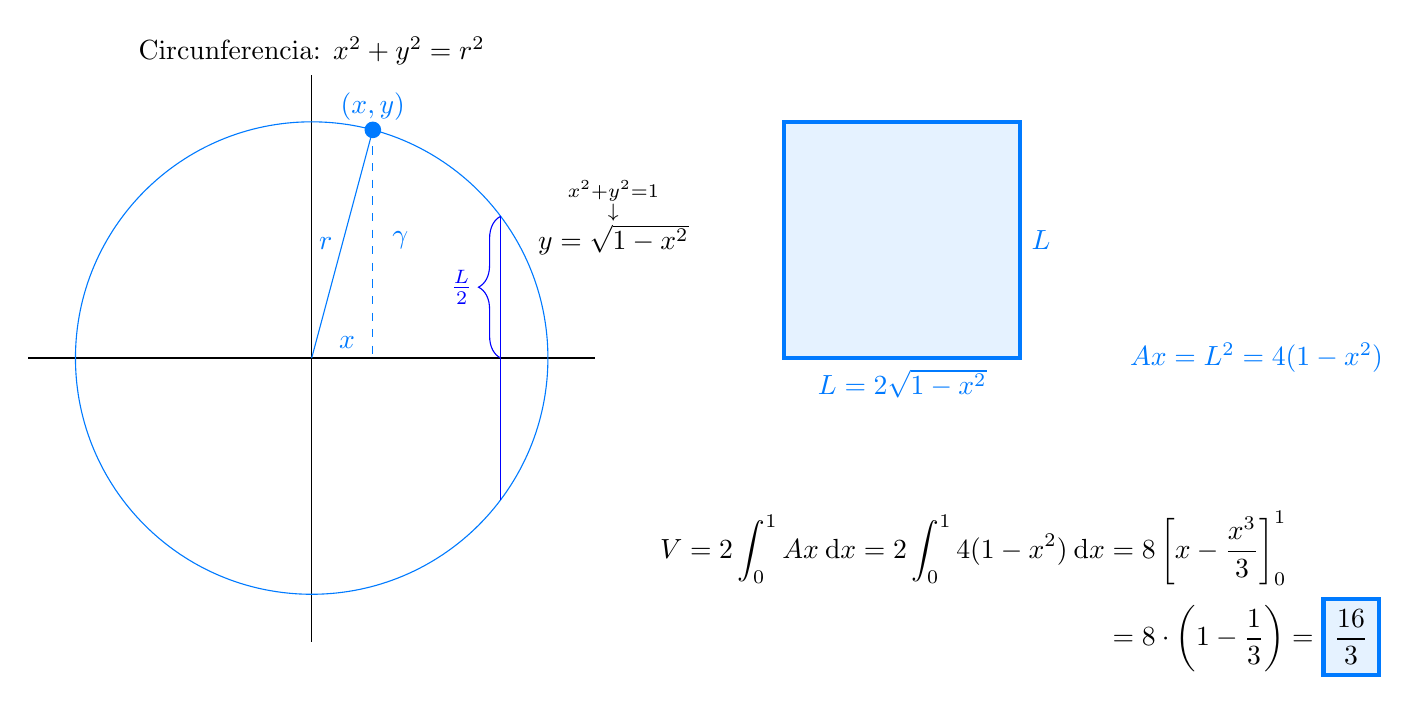
\begin{tikzpicture}[scale=3, decoration=brace]
            \draw[lightblue, dashed] (75:1) |- (0,0) ;
            \draw (-1.2,0) -- (1.2,0);
            \draw (0,-1.2) -- (0,1.2) node[above] {Circunferencia: $x^2+y^2=r^2$};
            \draw[lightblue] (0,0) circle (1);
            \draw[lightblue] (0,0) -- (75:1) node[midway, left] {$r$};
            \fill[lightblue] (75:1) circle (1pt) node[above] {$(x,y)$};
            \node[lightblue,above] at (0.15,0) {$x$};
            \node[lightblue, right] at (0.3,0.5) {$\gamma$};
            \draw[draw=blue] (0.8,0.6) node[right] {$\quad\overset{\begin{subarray}{c}
                              x^2+y^2=1\\
                              \downarrow
                  \end{subarray}}{\textstyle y=\sqrt{1-x^2}}$} -- (0.8,-0.6);
            \draw[blue, decorate, decoration={amplitude=8pt}] (0.8,0) -- (0.8,0.6) node[midway,left] {$\frac{L}{2}~~$};
            
            \draw[lightblue, fill=lightblue!10, line width=1.5] (2,1) -- (3,1) -- (3,0) node[midway,right] {$L$} -- (2,0) node[midway, below] {$L=2\sqrt{1-x^2}$} -- cycle;
            \node[lightblue] at (4,0) {$Ax=L^2=4(1-x^2)$};
            \node at (3,-1) {$\begin{aligned}
                        V=2\int_0^1Ax\dx=2\int_0^14(1-x^2)\dx&=8\left[x-\dfrac{x^3}{3}\right]_0^1\\
                        &=8\cdot\left(1-\dfrac{1}{3}\right)=\bboxed{\dfrac{16}{3}}
                  \end{aligned}$};
\end{tikzpicture}
\end{center}
\pagebreak
\item \lb{La base de un sólido es el círculo de centro (0,0) y radio 1 en el plano $XOY$. Sus secciones por planos perpendiculares al eje $OX$ son triángulos equilateros. Calcular el volumen del sólido.}
\begin{center}
      \begin{tikzpicture}[scale=3, decoration=brace]
            \draw[lightblue, dashed] (75:1) |- (0,0) ;
            \draw (-1.2,0) -- (1.2,0);
            \draw (0,-1.2) -- (0,1.2);
            \draw[lightblue] (0,0) circle (1);
            \draw[lightblue] (0,0) -- (75:1) node[midway, left] {$r$};
            \fill[lightblue] (75:1) circle (1pt) node[above] {$(x,y)$};
            \node[lightblue,above] at (0.15,0) {$x$};
            \node[lightblue, right] at (0.3,0.5) {$\gamma$};
            \draw[draw=blue] (0.8,0.6) node[right] {$\quad\overset{\begin{subarray}{c}
                              x^2+y^2=1\\
                              \downarrow
                  \end{subarray}}{\textstyle y=\sqrt{1-x^2}}$} -- (0.8,-0.6);
            \draw[blue, decorate, decoration={amplitude=8pt}] (0.8,0) -- (0.8,0.6) node[midway,left] {$\frac{L}{2}~~$};
            
            \draw[lightblue, line width=1.5, fill=lightblue!10] (2,0) -- ++(60:1) -- ++ (-60:1)  node[midway, right] {$L$} -- (2,0) node[midway, below] {$L=2\sqrt{1-x^2}$};
            \node[lightblue] at (4,0.5) {$\begin{array}{l}
                        \left(\dfrac{L}{2}\right)^2+h^2=L^2\\
                        h^2=L^2-\dfrac{L^2}{4}=\dfrac{3}{4}L^2\\
                        h=\dfrac{\sqrt{3}}{2}L=\dfrac{\sqrt{3}}{2}(2\sqrt{1-x^2})\\
                        h=\sqrt{3}\cdot\sqrt{1-x^2}
                  \end{array}$};
            \node[lightblue] at (2.7, 0.2) {$\dfrac{L}{2}$};
            \draw[blue, dashed] (2.5,0) -- (2.5,0.85) node[right, midway] {$h$};
            \node[lightblue] at (2,-1.5) {$V=2\int_0^1Ax\dx=2\int_0^1\sqrt{3}(1-x^2)\dx=2\sqrt{3}\left[x-\dfrac{x^3}{3}\right]_0^1=2\sqrt{3}\left(1-\dfrac{1}{3}\right)=\bboxed{\dfrac{4\sqrt{3}}{3}}$};
      \end{tikzpicture}
\end{center}
\item \lb{Sabiendo que $I=\int_{-\infty}^{+\infty}e^{-x^2}\dx=\sqrt{\pi}$, calcula las siguientes integrales}

\begin{enumerate}[label=\color{red}\alph*)]
      \item $\db{\int_{0}^{\infty}x^2e^{-x^2}\dx=}\lim_{t\to\infty}\int_0^tx^2e^{-x^2}\dx=\lb{(\ast)}$
      
      $\begin{array}{l}
            \int x^2e^{-x^2}=\int\lbb{x}{}\cdot\lbb{xe^{-x^2}}{}\dx=\left\{\begin{array}{ll}
                  u=x & \du=\dx\\
                  \dv=xe^{-x^2} & v=-\dfrac{1}{2}e^{-x^2}
            \end{array}\right\}=-\dfrac{1}{2}xe^{-2}+\dfrac{1}{2}\int e^{-x^2}\dx\\
            \lb{(\ast)=}\lim_{t\to\infty}\left(\left[-\dfrac{1}{2}xe^{-x^2}\right]_0^t+\dfrac{1}{2}\int_0^te^{-x^2}\dx\right)=\lbb{\lim_{t\to+\infty}-\dfrac{1}{2}re^{-t^2}}{I_1}+\dfrac{1}{2}\dbb{\int_{0}^{+\infty}e^{-x^2}\dx}{I_2}=\bboxed{\dfrac{\sqrt{\pi}}{4}}\\
            \lb{I_1=}\lim_{t\to+\infty}-\dfrac{1}{2}\cdot\dfrac{t}{e^{t^2}}=\left(\dfrac{\infty}{\infty}\right)=\{\text{L'Hôpital}\}=\lim_{t\to+\infty}-\dfrac{1}{2}\cdot\dfrac{1}{2te^{t^2}}=\dfrac{1}{\infty}=0\\
            \lb{I_2=}\int_{0}^{+\infty}e^{-x^2}\dx=\dfrac{1}{2}\int_{-\infty}^{+\infty}e^{-x^2}\dx=\dfrac{\sqrt{\pi}}{2}
      \end{array}$
      \item $\db{\int_{-\infty}^{+\infty}e^{-\frac{(x-\mu)^2}{2\sigma^2}}\dx=}\int_{-\infty}^{+\infty}e^{-\left[\frac{x-\mu}{\sqrt{2}\cdot\sigma}\right]^2}\dx=\sqrt{2}\cdot\sigma\cdot\int_{-\infty}^{+\infty}\dfrac{1}{\sqrt{2}\sigma}e^{-\left(\frac{x-\mu}{\sqrt{2}\sigma}\right)^2}\dx=\left\{\begin{array}{l}
            \dfrac{x-\mu}{2\sigma}=t\\
            \dfrac{1}{2\sigma}\dx=\dt
      \end{array}\right\}=\sqrt{2}\cdot\sigma\lbb{\int_{-\infty}^{+\infty}e^{-t^2}\dt}{\sqrt{\pi}}=\bboxed{\sqrt{2\pi}\cdot\sigma}$
      \item $\db{\int_{0}^{\infty}\dfrac{e^{-x}}{\sqrt{x}}\dx=}\left\{\textstyle\begin{array}{l}
            x=t^2\\
            \dx=2t\dt\\
            \text{Si }x=0\longrightarrow t=0\\
            \text{Si }x=+\infty\longrightarrow t=+\infty
      \end{array}\right\}=\int_{0}^{+\infty}\dfrac{e^{-t^2}}{t}2t\dt=2\cdot\int_{0}^{+\infty}e^{-t^2}\dt=2\cdot\left(\dfrac{1}{2}\int_{-\infty}^{+\infty}e^{-t^2}\dt\right)$\\
      $=\bboxed{\sqrt{\pi}}$
\end{enumerate}
\item \lb{Se defie la función gamma de Euler como $\Gamma(\alpha)=\int_{0}^{+\infty}e^{-x}x^{\alpha-1}\dx$, si $\alpha>0$.}
\begin{enumerate}[label=\color{lightblue}\arabic*)]
      \item \lb{Justifica por qué la integral converge cuando $\alpha>0$.}
      \begin{enumerate}[label=\color{lightblue}\arabic*)]
            \item Si $0<\alpha<1$
            
            $\int_{0}^{+\infty}\dfrac{e^{-x}}{x^{-\alpha}}\dx=\int_0^1\dfrac{e^{-x}}{x^{1-\alpha}}\dx+\int_{1}^{+\infty}\dfrac{e^{-x}}{x^{1-\alpha}}\dx$
            
            $\int_0^1\dfrac{e^{-x}}{x^{1-\alpha}}\dx$
            
            $\lim_{x\to0^+}\dfrac{\frac{e^{-x}}{x^{1-\alpha}}}{\frac{1}{x^{1-\alpha}}}=\lim_{x\to0^+}e^{-x}=1=\mathrm{cte}\neq0\longrightarrow$ Ambas integrales tienen el mismo carácter.
            
            Como $\int_0^1\dfrac{1}{x^{1-\alpha}}\dx$ es convergente $1-\alpha<1\longrightarrow\int_0^1\dfrac{e^{-x}}{x^{1-\alpha}}\dx$ es convergente.
            
            $\int_{1}^{+\infty}\dfrac{e^{-x}}{x^{1-\alpha}}\dx$
            
            $\lim_{x\to+\infty}\dfrac{\frac{e^{-x}}{x^{1-\alpha}}}{e^{-x}}=\lim_{x\to+\infty}\dfrac{1}{x^{1-\alpha}}=\dfrac{1}{\infty}=0\longrightarrow\int_{1}^{+\infty}\dfrac{e^{-x}}{x^{1-\alpha}}\dx<\int_{1}^{+\infty}e^{-x}\dx=\left[-e^{-x}\right]_1^{+\infty}=e^{-1}$ convergente
            
            Como $\int_{1}^{+\infty}e^{-x}\dx$ es convergente $\longrightarrow\int_{1}^{+\infty}\dfrac{e^{-x}}{x^{1-\alpha}}\dx$ es convergente.
            \item Si $\alpha=1\qquad\int_{0}^{+\infty}e^{-x}\dx=\left[-e^{-x}\right]_{0}^{+\infty}=1$ Convergente
            \item Si $\alpha>1\qquad\int_{0}^{+\infty}e^{-x}\cdot x^{\alpha-1}\dx$ 
            
            Convergente por integración por partes hasta que el exponentes de $x^{\alpha-1}$ sea entre 0 y 1.
      \end{enumerate}
      \item \lb{Demuestra (integrando por partes) que $\Gamma(\alpha+1)=\alpha\Gamma(\alpha)$, para todo $\alpha>0$, y deduce por inducción que $\Gamma(n+1)=n!$.}
      
      $\Gamma(\alpha+1)=\int_{0}^{+\infty}e^{-x}\cdot x^{\alpha}\dx=\left\{\begin{array}{ll}
            u=x^{\alpha} & \du=\alpha\cdot x^{\alpha-1}\\
            \dv=e^{-x}\dx & v=-e^{-x}
      \end{array}\right\}=\lbb{\left[ \tozero{-x^{\alpha}\cdot e^{-x}}\right]_{0}^{+\infty}}{\lb{(\ast)}}$
      
      $+\alpha\lbb{\int_{0}^{+\infty}e^{-x}\cdot x^{\alpha-1}\dx}{\Gamma(\alpha)}=\alpha\Gamma(\alpha)\longrightarrow\bboxed{\Gamma(\alpha+1)=\alpha\Gamma(\alpha)}$
      
      $\lb{(\ast)=}\lim_{x\to+\infty}\dfrac{x^{\alpha}}{e^x}=\left(\dfrac{\infty}{\infty}\right)=\{\text{L'Hôpital}\}=\lim_{x\to+\infty}\dfrac{\alpha x^{\alpha-1}}{e^x}=\left(\dfrac{\infty}{\infty}\right)=\cdots=0$
      
      Por inducción: $\Gamma(n+1)=n!$
      \begin{enumerate}[label=\color{lightblue}\roman*)]
            \item $\Gamma(2)=\int_{0}^{+\infty}x^{-x}\cdot x\dx=\lim_{t\to+\infty}\int_0^txe^{-x}\dx=\lb{(\ast)}$
            
            $\int xe^{-x}\dx=\left\{\begin{array}{ll}
                  u=x & \du=\dx\\
                  \dv=e^{-x}\dx & v=-e^{-x}
            \end{array}\right\}=-xe^{-x}+\int e^{-x}\dx=-xe^{-x}-e^{-x}$
            
            $\lb{(\ast)=}\lim_{t\to+\infty}\left[-xe^{-x}-e^{-x}\right]_0^t=\lim_{t\to+\infty}(\lbb{-te^{-t}}{\lb{(\ast\ast)}}-\tozero{e^{-t}}+1)=1\longrightarrow\Gamma(2)=1!\longrightarrow\bboxed{n=1}$
            
            $\lb{(\ast\ast)=}\lim_{t\to+\infty}\dfrac{-t}{e^t}=\left(\dfrac{\infty}{\infty}\right)=\{\text{L'Hôpital}\}=\lim_{t\to+\infty}-\dfrac{1}{e^t}=-\dfrac{1}{\infty}=0$
            \item Supuesto cierto que $\Gamma(n)=(n-1)!$. Veamos si se cumple para el caso $(n+1)$ \[ \Gamma(n+1)=n\cdot\Gamma(n)=n\cdot(n-1)!=n!\longrightarrow\Gamma(n+1)=n! \] La propiedad de que $\Gamma(n+1)=n!$ es cierta $\forall\:n\in\N$
      \end{enumerate}
     
      \item \lb{Calcula en términos de la función gamma.}
      \begin{enumerate}[label=\color{red}\alph*)]
            \item $\db{\int_0^{\infty}e^{-\sqrt[3]{x}}\dx}$
            
            $\int_{0}^{+\infty}e^{-\sqrt[3]{x}}\dx=\left\{\begin{array}{l}
                        x=t^3\\
                        \dx=3t^2\dt\\
                        \text{Si }x=0\longrightarrow t=0\\
                        \text{Si }x=+\infty\longrightarrow t=+\infty
                  \end{array}\right\}=\int_{0}^{+\infty}3t^2e^{-t}\dt=3\int_{0}^{+\infty}t^2e^{-t}\dt=3\Gamma(3)=3\cdot 2!=6$

            \item $\db{\int_{0}^{\infty}x^ne^{-\frac{x^2}{2}}\dx,\:n\in\N}$
            
            $\begin{aligned}
                  \int_{0}^{+\infty}x^ne^{-\frac{x^2}{2}}\dx&=\int_{0}^{+\infty}x^{n-1}\cdot xe^{-\frac{x^2}{2}}\dx=\left\{\begin{array}{l}
                        \dfrac{x^2}{2}=t\\
                        x\dx=\dt\\
                        \text{Si }x=0\longrightarrow t=0\\
                        \text{Si }x=+\infty\longrightarrow t=+\infty
                  \end{array}\right\}=\int_{0}^{+\infty}(\sqrt{2t})^{n-1}e^{-t}\dt\\
                  &=(\sqrt{2})^{n-1}\cdot\int_{0}^{+\infty}\underset{\begin{subarray}{c}
                              \downarrow\\
                              \alpha-1=\frac{n-1}{2}\\
                              \alpha=\frac{n+1}{2}
                  \end{subarray}}{t^{\frac{n-1}{2}}}\cdot e^{-t}\dt=(\sqrt{2})^{n-1}\cdot\Gamma\left(\dfrac{n+1}{2}\right)
            \end{aligned}$
            \item $\db{\int_0^1\dfrac{x^{b-1}}{\left(\log\left(\frac{1}{x}\right)\right)^{1-a}}\dx,\:a,b>0}$
            
            $\log\left(\dfrac{1}{x}\right)=t\longrightarrow e^{-t}$
      \end{enumerate}
\end{enumerate}
\item \lb{Estudiar si $f$ verifica las hipótesis del Teorema de Rolle en $[a,\,b]$:}
\begin{enumerate}[label=\color{red}\alph*)]
      \item $\db{f(x)=2x+\sin(x),\quad a=0,\quad b=\pi}$
      
      \begin{minipage}[l]{\textwidth}
            \begin{wrapfigure}{r}{0.45\textwidth}
                  \begin{tikzpicture}[baseline=(current bounding box.center)]
                        \node[red,draw=red,fill=red!10,line width=1.5pt,text width=6cm] {\underline{Nota:} El teorema de Rolle dice que si $f(x)$ es continua en $[a,b]$, derivable en $(a,b)$ y además $f(a)=f(b)$, entonces se cumple que $\exists c\in(a,b)$ tal que $f'(c)=0$.};
                  \end{tikzpicture}
            \end{wrapfigure}
            
            $f(x)=2x+\sin(x)\quad I[0,\pi]$
            
            \quad\textbullet\quad $f(x)$ es continua en $[0,\pi]$
            
            \quad\textbullet\quad $f'(x)=2+\cos(x)\longrightarrow f(x)$ es derivable en $(0,\pi)$
            
            \quad\textbullet\quad $f(0)=0$ y $f(\pi)=2\pi$
            
            No verifica las hipótesis del teorema de Rolle.
      \end{minipage}
      \item $\db{f(x)=1-(1-x)^{\frac{1}{3}}\quad a=0,\quad b=2}$
      
      $f(x)=1-(1-x)^{\frac{1}{3}}\quad I=[0,2]$
      \begin{itemize}
            \item $f(x)$ es continua en $[0,2]$
            \item $f'(x)=-\dfrac{1}{3}(1-x)^{-\frac{2}{3}}=-\dfrac{1}{3\sqrt[3]{(1-x)^2}}$ a problemas en $x=1\longrightarrow f(x)$ no es derivable en $(0,2)$
      \end{itemize}
\end{enumerate}
\item \lb{Utiliza el teorema de Rolle para averiguar cuántas raíces reales tienen los siguientes polinomios.}
\begin{enumerate}[label=\color{red}\alph*), leftmargin=*]
      \item $\db{6x^5+13x-1}$
      
\begin{minipage}[l]{0.5\textwidth}
            $\begin{array}{l}
                  f(x)=6x^5-13x-1\\
                  f'(x)=30x^4+13\neq0
            \end{array}$
            
            Como no hay puntos con $f'(x)=0$ entonces por el teorema de Rolle si hay alguna raíz, esta deberá ser única.
            
            $\begin{rcases}
                  f(0)=-1<0\\
                  f(1)=18>0
            \end{rcases}$ Por el Teorema de Bolzano $\exists c\in(0,1)$ tal que $f(c)=0$.
            
\begin{center}
      \includegraphics[width=0.7\textwidth]{Imágenes/119.png}
\end{center}

      $\begin{array}{l}
            I=[0,1]\longrightarrow x_m=\dfrac{1}{2}\longrightarrow f\left(\dfrac{1}{2}\right)=5.6875>0\\
            I=\left[0,\dfrac{1}{2}\right]\longrightarrow x_m=\dfrac{1}{4}\longrightarrow f\left(\dfrac{1}{4}\right)=2.2558>0
      \end{array}$
\end{minipage}\quad
\begin{minipage}[l]{0.45\textwidth}
            \begin{tikzpicture}[baseline=(current bounding box.center)]
                  \node[red,draw=red,fill=red!10,line width=1.5pt,text width=8cm] {\underline{Nota:} El teorema de Rolle se utiliza mucho para justificar cuántas raices podría haber. Si hacemos la derivada de la función $f(x)$, la igualo a cero y saco los puntos críticos $\left(f'(x)=0\right)$. Si partimos la recta real en función de estos puntos\begin{center}
                              \begin{tikzpicture}
                                    \draw (-2,0) node[left] {$-\infty$} -- (2,0) node[right] {$+\infty$};
                                    \draw (-1,0.1) -- (-1,-0.1) node[below] {$a$};
                                    \draw (0,0.1) -- (0,-0.1) node[below] {$b$};
                                    \draw (1,0.1) -- (1,-0.1) node[below] {$c$};
                              \end{tikzpicture}\\
                              $f'(A)=f'(b)=f'(c)=0$
                  \end{center}
                  \begin{minipage}{0.5\textwidth}
                        $\begin{array}{l}
                              I_1=(-\infty, a]\\
                              I_2=[a,b]\\
                              I_3=[b,c]\\
                              I_4=[c,+\infty)
                        \end{array}$
                  \end{minipage}\begin{minipage}{0.5\textwidth}
                  Por Rolle podremos asegurar que en cada intervalo habrá una o ninguna raíz (Bolzano)
                  \end{minipage}\\
                  Sólo habrá una o ninguna, ya que si hubieran dos raíces $f(\alpha)=f(\beta)=0$ entre medias por Rolle habría $f'(c)=0$, pero no lo hay.
            };
            \end{tikzpicture}
\end{minipage}

$\begin{array}{l}
      I=\left[0,\dfrac{1}{4}\right]\longrightarrow x_m=\dfrac{1}{8}\longrightarrow f\left(\dfrac{1}{8}\right)=0.62518>0\\
      I=\left[0,\dfrac{1}{8}\right]\longrightarrow x_m=\dfrac{1}{16}\longrightarrow f\left(\dfrac{1}{16}\right)=-0.1875<0\\
      I=\left[\dfrac{1}{16},\dfrac{1}{8}\right]=\left[0.0625,\,0.125\right]\longrightarrow x_m=0.09375\longrightarrow f(0.09375)=0.21879>0\\
      I=[0.0625,\,0.09375]
\end{array}$

\item $\db{x^4-4x+1}$

$\begin{array}{l}
      f(x)=x^4-4x+1\\
      f'(x)=4x^3-4=0\longrightarrow x^3-1=0\longrightarrow x=1
\end{array}$

\begin{center}
      \begin{tikzpicture}
            \draw (-1,0) node[left] {$-\infty$} -- (3,0) node[right] {$+\infty$};
            \draw (1,0.1) -- (1,-0.1) node[below] {$1$};
            \node at (-1,-1) {$\begin{array}{l}
                        I_1=(-\infty,1]\\
                        I_2=[1,+\infty)
                  \end{array}$};
            \node[text width=8cm] at (5,-1.2) {En cada uno de estos intervalos, por Rolle, si hay alguna raíz, esta sería única.};
      \end{tikzpicture}
\end{center}
\begin{itemize}[leftmargin=3cm]
      \item[$\underline{I_1=(-\infty,1]}$] $\begin{rcases}
            \lim_{x\to-\infty}f(x)=\lim_{x\to-\infty}(x^4-4x+1)=+\infty>0\longrightarrow f(-1)=6>0\\
            f(1)=-2<0
      \end{rcases}$ 
      
      Por Bolzano $\exists c_1\in(-1,1)$ tal que $\bboxed{f(c_1)=0}$
      \item[$\underline{I_2=[1,+\infty)}$] $\begin{array}{l}
            f(-1)=-2<0\\
            \lim_{x\to+\infty}f(x)=+\infty\longrightarrow f(2)=9>0
      \end{array}$
      
      Por Bolzano $\exists c_2\in(1,2)$ tal que $\bboxed{f(c_2)=0}$
\end{itemize}
La función tiene 2 raíces
\item $\db{x^3-3x+a=0\text{ en }[-1,1]}$

$\begin{array}{l}
      f(x)=x^3-3x+a\qquad x\in[-1,1]\\
      f'(x)=3x^2-3=0\longrightarrow x^2-1=0\longrightarrow x=\pm1
\end{array}$

\begin{center}
	\begin{tikzpicture}[baseline=(current bounding box.center),scale=1.5]
      \draw (-2,0) -- (2,0);
      \draw (-0.8,0.2) -- (-1,0.2) -- (-1,-0.2) node[below] {$-1$} -- (-0.8,-0.2);
      \draw (0.8,0.2) -- (1,0.2) -- (1,-0.2) node[below] {$1$} -- (0.8,-0.2);
      \draw[latex-] (0,0.1) -- (0.1,0.5) node[above right] {entre medias $f'(x)\neq0$};
\end{tikzpicture}\qquad
\begin{minipage}[l]{7cm}
	Por el teorema de Rolle, podemos asegurar que en este intervalo, si hay alguna raíz esta deberá ser única
\end{minipage}
\end{center}
$ \begin{aligned}
	\begin{rcases}
		f(-1)=2+a\\
		f(1)=-2+a
	\end{rcases}&(-1)\cdot f(1)<0\text{ (Condición para que se cumpla Bolzano y haya raíz)}\\
	&(1+a)(-2+a)<0\\
	&a^2-4<0\longrightarrow a^2<4\longrightarrow\bboxed{a\in(-2,2)}\lb{\longrightarrow\text{ Si hay raíz}}
\end{aligned}$

\fcolorbox{lightblue}{lightblue!10}{\begin{minipage}[l]{12cm}
		$f(x)$ tiene una única raíz en $[-1,1]$ si $a\in[-2,2]$.\\
		$f(x)$ no tiene ninguna raíz en $[-1,1]$ si $a\in(-\infty,-2)\cup(2,+\infty)$.
\end{minipage}}
\end{enumerate}
\lb{Utiliza Bolzano para encontrar un intervalo donde estén las raíces, y el método de la bisección para estimar su valor. En $c)$, determina sólo para qué valores de $a$ existe exactamente 1 raíz.}


\item \lb{Estudiar la convergencia y sumar la siguiente serie: \[ \sum_{n=1}^{\infty}\dfrac{3n+1}{5^n} \]}

Para estudiar la convergencia aplicaremos el criterio del cociente: \begin{center}
	\begin{minipage}[l]{15cm}
		$\lim_{n\to\infty}\dfrac{a_{n+1}}{a_n}=\lim_{n\to\infty}\dfrac{\frac{3(n+1)+1}{5^{n+1}}}{\frac{3n+1}{5^n}}=\lim_{n\to\infty}\dfrac{(3n+4)\cdot\cancel{5^n}}{(3n+1)\cdot5^n\cdot5}=\lim_{n\to\infty}\dfrac{3n+4}{15n+5}=\left(\dfrac{\infty}{\infty}\right)=\lim_{n\to\infty}\dfrac{\frac{3n}{n}+\cancel{\frac{4}{n}}}{\frac{15n}{n}+\cancel{\frac{5}{n}}}=\dfrac{3}{15}=\dfrac{1}{5}<1\longrightarrow$ La serie es convergente
	\end{minipage}
\end{center}
$\sum_{n=1}^{\infty}\dfrac{3n+1}{5^n}=\sum_{n=1}^{\infty}(3n+1)\left(\dfrac{1}{5}\right)^n=\sum_{n=1}^{\infty}a_nb_n=\lim_{n\to\infty}\lbb{\sum_{j=1}^{n}a_jb_j}{S_n}=\lb{(\ast)}$

$a_n=3n+1\longrightarrow$ progresión aritmétrica $(d=3)$\\
$b_n=\left(\dfrac{1}{5}\right)^n\longrightarrow$ progresión geométrica $\left(r=\dfrac{1}{5}\right)$

\[ \begin{array}{l}
	\begin{array}{ll}
		S_n=a_1b_1+&a_2b_2+a_3b_3+\cdots+a_nb_n\\
		rS_N=&a_1b_2+a_2b_3+\cdots+a_{n-1}b_n+a_nb_{n+1}\\ \hline
		\multicolumn{2}{l}{(1-r)S_n=a_1b_1+\lbb{(a_2-a_1)}{d}b_2+\lbb{(a_3-a_2)}{d}b_3+\cdots+\lbb{(a_n-a_{n-1})}{d}b_n-a_nb_{n+1}}
	\end{array}\\
	(1-r)S_n=a_1b_1+d\underset{\begin{array}{c}
			\rotatebox{90}{=}\\
			\frac{b_2-b_nr}{1-r}
	\end{array}}{(b_2+b_3+\cdots+b_n)}-a_nb_{n+1}\\
\bboxed{S_n=\dfrac{a_1b_1}{1-r}+d\dfrac{b_2-b_nr}{(1-r)^2}-\dfrac{a_nb_{n+1}}{1-r}}
\end{array} \]
$\lb{(\ast)=}\lim_{n\to\infty}\left(\dfrac{4\cdot\frac{1}{5}}{1-\frac{1}{5}}+3\dfrac{\left(\frac{1}{5}\right)^2-\tozero{\left(\frac{1}{5}\right)^n\cdot\frac{1}{5}}}{\left(1-\frac{1}{5}\right)^2}-\tozero{\dfrac{(3n+1)\cdot\left(\frac{1}{5}\right)^{n+1}}{1-\frac{1}{5}}}\right)=\dfrac{\frac{4}{5}}{\frac{4}{5}}+3\dfrac{\frac{1}{25}}{\frac{1}{25}}=1+\dfrac{3}{16}=\bboxed{\dfrac{19}{16}}$
\item \lb{Considera la sucesión recurrente dada por $a_{n+1}=\sqrt{a_n+a_n^2}$, con $a_1=1$.}
\begin{enumerate}[label=\color{red}\roman*)]
	\item \db{Demuestra que $a_n$ es creciente}
	
	$\dfrac{a_{n+1}}{a_n}=\dfrac{\sqrt{a_n+a_n^2}}{a_n}=\sqrt{\dfrac{a_n+a_n^2}{a_n^2}}=\sqrt{\dfrac{1}{a_n}+1}>1\longrightarrow a_{n+1}>a_n\:\forall n\in\N$
	
	$a_n$ es creciente $\forall n\in\N$
	\item \db{Demuestra que $\lim a_n=+\infty$.}
	
	Supongamos que $a_n$ está acotada inferiormente $\longrightarrow a_n$ sería convergente.
	
	Por lo tanto: $\lim_{n\to\infty}a_n=\lim_{n\to\infty}a_{n+1}=L=\mathrm{cte}$ \[ a_{n+1}=\sqrt{a_n+a_n^2}\longrightarrow L=\sqrt{L+L^2}\longrightarrow \cancel{L^2}=L+\cancel{L^2}\longrightarrow L=0\rc{\text{!! (Imposible)}} \]Por lo tanto, lo que hemos supuesto cierto, en verdad es falso $\longrightarrow a_n$ no está acotada superiormente $\longrightarrow\lim_{n\to\infty}a_n=+\infty$.
	\item \db{Utiliza Stolz (justificadamente) para calcular $\lim\dfrac{a_n}{n}$}
	
	$\lim_{n\to\infty}\dfrac{a_n}{n}=\left(\dfrac{\infty}{\infty}\right)=\{\mathrm{Stolz}\}=\lim_{n\to\infty}\dfrac{a_{n+1}-a_n}{n+1-n}=\lim_{n\to\infty}(a_{n+1}-a_n)=\lim_{n\to\infty}(\sqrt{a_n+a_n^2}-a_n)=\linebreak(\infty-\infty)=\lim_{n\to\infty}\dfrac{(\sqrt{a_n+a_n^2}-a_n)\cdot(\sqrt{a_n+a_n^2}+a_n)}{\sqrt{a_n+a_n^2}+a_n}=\lim_{n\to\infty}\dfrac{(\sqrt{a_n+a_n^2})^2-a_n^2}{\sqrt{a_n+a_n^2}+a_n}=\lim_{n\to\infty}\dfrac{a_n+\cancel{a_n^2}-\cancel{a_n^2}}{\sqrt{a_n+a_n^2}+a_n}\linebreak=\lim_{n\to\infty}\dfrac{a_n}{\sqrt{a_n+a_n^2}+a_n}=\left(\dfrac{\infty}{\infty}\right)=\lim_{n\to\infty}\dfrac{1}{\sqrt{\tozero{\frac{1}{a_n}}+1}+1}=\bboxed{\dfrac{1}{2}}$
\end{enumerate}
\item \lb{Sea $(a_n)_n$ una sucesion de números reales. Establecer una condición necesaria y suficiente para que la serie $\sum_{n=1}^{\infty}(a_{n+2}a_n)$ sea convergente.}

$\sum_{n=1}^{\infty}(a_{n+2}-a_n)=\lim_{n\to\infty}\lbb{\sum_{j=1}^{n}(a_{j+2}-a_j)}{S_n}=\lb{(\ast)}$

$S_n=(\cancel{a_3}-a_1)+(\cancel{a_4}-a_2)+(a_5-\cancel{a_3})+(a_6-\cancel{a_4})+(\cancel{a_7}-\cancel{a_5})+\cdots+(a_{n+1}-\cancel{a_{n-1}})+(a_{n+2}-\cancel{a_n})=a_{n+1}+a_{n+2}-a_1-a_2$

$\lb{(\ast)=}\lim_{n\to\infty}(a_{n+1}+a_{n+2}-a_1-a_2)$

La condición necesaria y suficiente para que sea convergente es que $\lim_{n\to\infty}a_n=L=\mathrm{cte}$
\item \lb{Obtener los desarrollos en series de potencias de las siguientes funciones:}

$\db{f(x)=e^{-x^2}}$

$\begin{array}{l}
	g(x)=e^x=1+x+\dfrac{x^2}{2!}+\dfrac{x^3}{3!}+\dfrac{x^4}{4!}=\sum_{n=0}^{+\infty}\dfrac{x^n}{n!}\\
	f(x)=e^{-x^2}=\sum_{n=0}^{+\infty}\dfrac{(-x^2)^n}{n!}=\sum_{n=0}^{+\infty}\dfrac{(-1)^n\cdot x^{2n}}{n!}\longrightarrow \bboxed{e^{-x^2}=\sum_{n=0}^{+\infty}\dfrac{(-1)^n\cdot x^{2n}}{n!}}
\end{array}$
\item \lb{Construir el desarrollo de Taylor de orden 3 de $f(x)=\sqrt[3]{4+x}$ centrado en $x_0=4$.}

$\begin{array}{l}
	T_4(x)=f(4)=\dfrac{f'(4)}{1!}(x-4)+\dfrac{f''(4)}{2!}(x-4)^2+\dfrac{f'''(4)}{3!}(x-4)^3\\
	f(x)=\sqrt[3]{4+x}=(4+x)^{\frac{1}{3}}\longrightarrow f(4)=2\\
	f'(x)=\dfrac{1}{3}(4+x)^{\frac{2}{3}}=\dfrac{1}{3\sqrt[3]{(4+x)^2}}\longrightarrow f'(4)=\dfrac{1}{12}\\
	f''(x)=-\dfrac{2}{9}(4-x)^{-\frac{5}{3}}=\dfrac{-2}{9\sqrt[3]{(4+x)^5}}\longrightarrow f''(4)=\dfrac{-2}{0\cdot32}=-\dfrac{1}{144}\\
	f'''(x)=\dfrac{10}{27}(4+x)^{-\frac{8}{3}}=\dfrac{10}{27\sqrt[3]{(4+x)^8}}\longrightarrow f'''(4)=\dfrac{10}{27\cdot2^8}=\dfrac{5}{3456}\\
	\bboxed{T_3(x)=2+\dfrac{1}{12}(x-4)-\dfrac{1}{288}(x-4)^2+\dfrac{5}{20736}(x-4)^3}
\end{array}$

\begin{itemize}[label=\color{red}\textbullet, leftmargin=*]
	\item \color{lightblue}Utilizar este desarrollo para calcular un valor aproximacdo de $\sqrt[3]{8.2}$ y acotar el error cometido en la aproximación.
\end{itemize}

$\begin{array}{l}
	f(x)=\sqrt[3]{4+x}=\sqrt[3]{8.2}\longrightarrow4+x=8.2\longrightarrow\bboxed{x=4.2}\\
	T_3(x=4.2)=2+\dfrac{1}{12}(0.2)-\dfrac{1}{288}(0.2)^2+\dfrac{5}{20736}(0.2)^3 =2.0,165297\\
	\bboxed{\sqrt[3]{8.2}\simeq2.0165297}\\
\end{array}$

$R_3(x)=\left|\dfrac{f^{\mathrm{iv}}(c)}{4!}(x-4)^4\right|=\underset{4<c<4.2}{\left|\dfrac{\frac{-80}{81\sqrt[3]{(4+x)^{11}}}}{24}(4.2-4)^4\right|}=\underset{\begin{subarray}{c}
		\downarrow\\
		\text{acotamos $c$ por su}\\
		\text{cota inferior}
\end{subarray}}{\dfrac{80}{1944\sqrt[3]{(4+x)^{11}}}(0.2)^4}<\dfrac{80}{1944\cdot2^{11}}(0.2)^4=\bboxed{32.15\cdot10^{-9}}$

$f(x)=-\dfrac{80}{81}(4+x)^{-\frac{11}{3}}=-\dfrac{80}{81\sqrt[3]{(4+x)^{11}}}$
\item $\lb{\int\dfrac{1}{x^2+4x+8}\dx}$

$\int\dfrac{1}{x^2+4x+8}\dx=\int\dfrac{1}{(x+2)^2+4}\dx=\int\dfrac{\frac{1}{4}}{\frac{(x+2)^2}{4}+1}\dx=\dfrac{1\cdot2}{4}\int\dfrac{\frac{1}{4}}{\left(\frac{(x+2)}{2}\right)^2+1}\dx=\left\{\begin{array}{l}
	\dfrac{x+2}{2}=t\\
	\dfrac{1}{2}\dx=\dt
\end{array}\right\}=\dfrac{1}{2}\int\dfrac{1}{t^2+1}\dt=\dfrac{1}{2}\arctan(t)+\mathrm{C}=\bboxed{\dfrac{1}{2}\arctan\left(\dfrac{x+2}{2}\right)+\mathrm{C}}$

$\begin{array}{l}
	x^2+4x+8=0\longrightarrow x=\dfrac{-4\pm\sqrt{16-32}}{2}=\nexists\\
	x^2+4x+8=(x^2+4x+4)+4=(x+2)^2+4\\
	(x+a)^2=x^2+2ax+a^2=x^2+4x+4\\
	2a-4\longrightarrow a=2
\end{array}$
\item \lb{Sea $f$ una función derivable que cumple \[ \int_{0}^{x}f(t)\dt=-10+x^2+x\sin(2x)+\dfrac{1}{2}\cos(2x). \]Calcula $f\left(\dfrac{\pi}{4}\right)$ y $f'\left(\dfrac{\pi}{4}\right)$}

Para encontrar $f(x)$ nos va a interesar derivar toda la ecuación: \[ \begin{array}{l}
	\left(\int_0^xf(t)\dt\right)'=f(x)\cdot1-\cancel{f(0)\cdot0}=f(x)\\
	\left(-10+x^2+x\sin(2x)+\dfrac{1}{2}\cos(2x)\right)'=2x+\cancel{\sin(2x)}+2x\cos(2x)-\cancel{\sin(2x)}=2x(1+\cos(2x))
\end{array} \]Por lo tanto: $f(x)=2x(1+\cos(2x))$\[ \bboxed{f\left(\dfrac{\pi}{4}\right)=2\dfrac{\pi}{4}\left(1+\cancel{\cos\left(\dfrac{\pi}{2}\right)}\right)=\dfrac{\pi}{2}} \]$f'(x)=2(1+\cos(2x))+2x(-2\sin(2x))\longrightarrow\bboxed{f'\left(\dfrac{\pi}{4}\right)=2\left(1+\tozero{\cos\left(\dfrac{\pi}{2}\right)}\right)+2\dfrac{\pi}{4}\left(-2\sin\left(\dfrac{\pi}{2}\right)\right)=2-\pi}$

\item \lb{Estudiar la convergencia de: \[ \sum_{n=1}^{\infty}\log\left(n\sin\left(\dfrac{1}{n}\right)\right) \]}
Aplicando Taylor: $\sin(x)=x-\dfrac{x^3}{6}\longrightarrow\sin\left(\dfrac{1}{n}\right)=\dfrac{1}{n}-\dfrac{1}{6n^3}$

$\sum_{n=1}^{\infty}\log\left(n\sin\left(\dfrac{1}{n}\right)\right)=\sum_{n=1}^{\infty}\log\left(n\left(\dfrac{1}{n}-\dfrac{1}{6n^3}\right)\right)=\sum_{n=1}^{\infty}\log\left(1-\dfrac{1}{6n^2}\right)=\left\{\log(1+x)\leadsto_0 x\right\}=\sum_{n=1}^{\infty}\left(-\dfrac{1}{6n^2}\right)=-\dfrac{1}{6}\sum_{n=1}^{\infty}\dfrac{1}{n^2}\longrightarrow$ Convergente
\item \lb{Obtener los desarrollos en series de potencias de las siguientes funciones:}

$\db{f(x)=\cos^2(x)=}\dfrac{1+\cos(2x)}{2}=\dfrac{1}{2}+\dfrac{1}{2}\cos(2x)$

Sabemos que $\cos(x)=\sum_{n=0}^{+\infty}(-1)^n\cdot\dfrac{x^{2n}}{(2n)!}\longrightarrow\cos(2x)=\sum_{n=0}^{+\infty}(-1)^n\cdot\dfrac{(2x)^{2n}}{(2n)!}=\sum_{n=0}^{+\infty}(-1)^n\cdot\dfrac{2^{2n}\cdot x^{2n}}{(2n)!}$

Por lo tanto: \[ \bboxed{f(x)=\dfrac{1}{2}+\dfrac{1}{2}\cdot\sum_{n=0}^{+\infty}(-1)^n\cdot\dfrac{2^{2n}\cdot x^{2n}}{(2n)!}} \]
\item \lb{Obtener los desarrollos en series de potencias de las siguietnes funciones:}

$\db{f(x)=\dfrac{1}{(1-x)^2}}$

\begin{minipage}[l]{\textwidth}
	\begin{wrapfigure}{r}{0.35\textwidth}
		\begin{tikzpicture}[baseline=(current bounding box.center)]
			\node[red,draw=red,fill=red!10,line width=1.5pt,text width=6cm] {\underline{Nota:} Serie Geométrica\[ \sum_{n=0}^{+\infty}r^n=\dfrac{1}{1-r}\:|r|<1 \]};
		\end{tikzpicture}
	\end{wrapfigure}
	
	$\dfrac{1}{1-x}=\sum_{n=0}^{+\infty}x^n$ si $|x|<1$
	
	Derivando: 
	
	$\begin{rcases}
		\left(\dfrac{1}{1-x}\right)'=\dfrac{1}{(1-x)^2}\\
		\left(\sum_{n=0}^{+\infty}x^n\right)'=\sum_{n=0}^{+\infty}nx^{n-1}
	\end{rcases}\longrightarrow\bboxed{\dfrac{1}{(1-x)^2}=\sum_{n=0}^{+\infty}nx^{n-1}\text{ si }|x|<1}$
	
	
\end{minipage}

\item \lb{Obtener los desarrollos en series de potencias de las siguientes funciones:}

$\db{f(x)=\log\left(\sqrt{\dfrac{1+x}{1-x}}\right)=}\log\left(\dfrac{1+x}{1-x}\right)^{\frac{1}{2}}=\dfrac{1}{2}\left[\log(1+x)-\log(1-x)\right]$

Como sabemos que: \[ \begin{array}{l}
	\log(1+x)=\sum_{n=1}^{+\infty}(-1)^{n+1}\cdot\dfrac{x^n}{n}\text{ si }|x|<1\\
	\log(1-x)=\sum_{n=1}^{+\infty}(-1)^{n+1}\cdot\dfrac{(-x)^n}{n}\text{ si }|-x|<1\longrightarrow|x|<1
\end{array} \]$\bboxed{\begin{aligned}
		f(x)&=\dfrac{1}{2}\left[\sum_{n=1}^{\infty}(-1)^{n+1}\cdot\dfrac{x^n}{n}-\sum_{n=1}^{\infty}(-1)^{n+1}\cdot\dfrac{(-1)^n\cdot x^n}{n}\right]\\
		&=\dfrac{1}{2}\sum_{n=1}^{\infty}(-1)^{n+1}\cdot\dfrac{x^n}{n}\cdot(1-(-1)^n)\text{ si }|x|<1
\end{aligned}}$
\item \lb{Calcular la derivada de $f(x)=x^{\sin(x)}$}

\begin{minipage}[l]{\textwidth}
	\begin{wrapfigure}{r}{0.5\textwidth}
		\begin{tikzpicture}[baseline=(current bounding box.center)]
			\node[red,draw=red,fill=red!10,line width=1.5pt,text width=8cm] {\underline{Nota:} Cunado tengamos que derivar una función exponencial, pero donde tanto base como exponente dependen de $x$, lo que haremos será aplicar derivación logarítmica que consiste en meter logaritmos a ambos lados y derivar.};
		\end{tikzpicture}
	\end{wrapfigure}
	
	$\log\left(f(x)\right)=\log\left(x^{\sin(x)}\right)=\sin(x)\cdot\log(x)$
	
	Derivamos: 
	
	$\begin{array}{l}
		\dfrac{1}{f(x)}\cdot f'(x)=\cos(x)\cdot\log(x)+\sin(x)\cdot\dfrac{1}{x}\\
		f'(x)=f(x)\left[\cos(x)\cdot\log(x)+\dfrac{\sin(x)}{x}\right]
	\end{array}$
	
	$\bboxed{f'8x)=x^{\sin(x)}\left[\cos(x)\cdot\log(x)+\dfrac{\sin(x)}{x}\right]}$
\end{minipage}

\vspace{1cm}

\item \lb{Calcular la recta tangente en el punto $x=1$ de la función $f(x)=x^x$.}

La recta tangente viene dada por: \begin{center}
	$y-b=m(x-a)$ donde $m=f'(a)$
\end{center}
$\begin{array}{l}
	a=1\\
	b=f(a)=f(1)=1
\end{array}$

Para derivar aplicamos derivación logarítimica: \[ \log\left(f(x)\right)=\log(x^x)=x\log(x) \]Derivamos:\[ \begin{array}{l}
	\dfrac{1}{f(x)}\cdot f'(x)=\log(x)+x\cdot\dfrac{1}{x}=1+\log(x)\\
	f'(x)=f(x)\left[1+\log(x)\right]\longrightarrow f'(x)=x^x\left[1+\log(x)\right]\longrightarrow f'(1)=1\cdot\left[1+\log(1)\right]=1
\end{array} \] La recta tangente es: \[ y-1=1\cdot(x-1)\longrightarrow\bboxed{y=x} \]
\end{enumerate}
\end{document}

\begin{minipage}[l]{\textwidth}
      \begin{wrapfigure}{r}{0.35\textwidth}
            \begin{tikzpicture}[baseline=(current bounding box.center)]
                  \node[red,draw=red,fill=red!10,line width=1.5pt,text width=6cm] {};
            \end{tikzpicture}
      \end{wrapfigure}
\end{minipage}